\documentclass[12pt]{article}
\usepackage{a4wide}
\usepackage{amsmath,amssymb}
\usepackage{bm}
\usepackage[colorlinks]{hyperref}
\usepackage{graphicx}



\usepackage{float}
\usepackage{bbold}
\usepackage{comment}
\usepackage{mathtools}


%\usepackage{caption,refstyle}

% Package diagramme Processus de Production de la GS
\usepackage{tikz}
\usetikzlibrary{positioning, shadows}


\usepackage[french]{babel}
\usepackage[T1]{fontenc}
\usepackage{lmodern}

\DeclareUnicodeCharacter{2009}{\,} 
\usepackage[standard]{ntheorem}



\usepackage{tikz}
\usepackage{graphicx}
\usetikzlibrary{positioning, arrows.meta}
\usepackage{amsmath}
\usepackage{pdfpages}
\usepackage{adjustbox}
\usepackage{appendix}




% ----- Recette

\usepackage{listings}
\usepackage{xcolor} % Pour la coloration syntaxique personnalisée
\usepackage{calc}


\lstdefinestyle{python}{
    language=Python,
    basicstyle=\ttfamily\footnotesize,
    keywordstyle=\color{blue},
    stringstyle=\color{green},
    commentstyle=\color{gray},
    numbers=left,
    numberstyle=\tiny\color{gray},
    stepnumber=1,
    numbersep=10pt,
    showstringspaces=false,
    frame=single,
    breaklines=true,
    breakatwhitespace=true,
    tabsize=4,
}

\lstset{
    inputencoding=utf8,
    extendedchars=true,
    literate={é}{{\'e}}1 {è}{{\`e}}1 {ê}{{\^e}}1 {ç}{{\c{c}}}1,
    % Autres caractères spéciaux peuvent être ajoutés ici
    language=Python,                     % Langage du code
    basicstyle=\footnotesize\ttfamily,   % Taille et style de police
    keywordstyle=\color{blue},           % Style des mots-clés
    stringstyle=\color{red},             % Style des chaînes de caractères
    commentstyle=\color{green!50!black}, % Style des commentaires
    showspaces=false,                    % Ne pas montrer les espaces
    showstringspaces=false,              % Ne pas montrer les espaces dans les chaînes
    breaklines=true,                     % Permettre les retours à la ligne automatiques
    tabsize=2,                           % Taille des tabulations
    captionpos=b,                        % Position de la légende (b pour en bas)
    numbers=left,                        % Numérotation des lignes à gauche
    numberstyle=\tiny\color{gray},       % Style des numéros de ligne
    escapeinside={(*}{*)},  
}




\usepackage{listings}
\usepackage{xcolor}
\usepackage{calc}


\usepackage{algorithm2e}

% \usepackage{algorithm}
% \usepackage{algorithmic}


\usepackage{enumitem}




\begin{document}


% Page de garde
\begin{titlepage}
    \centering
    
    % Titre du rapport
    {\Huge \textbf{Rapport de Stage de Fin d'Études}} \\[1.5cm]
    % {\LARGE Master 2 Mathématiques Appliquées} \\[1cm]
    {\large \textbf{Sujet du stage }} \\
    {\Large Optimisation des coûts de production} \\[2cm]
    
    % Nom de l'étudiant
    {\Large \textbf{Présenté par }} \\
    {\Large Job CONGO} \\[1cm]
    
    % Détails du stage
    {\large \textbf{Stage réalisé à }} \\
    {\large Fonderie de Niederbronn, Niederbronn, France} \\[0.5cm]

    % Dates du stage
    {\large \textbf{Dates du stage }} \\
    {\large Du 11 mars 2024 au 26 juillet 2024} \\[1cm]

    {\large \textbf{Encadrant industriel }} \\
    {\large Guy LUTRINGER, président de la Fonderie de Niederbronn} \\[0.5cm]
    

    % Université et laboratoire
    {\large \textbf{Responsable académique }} \\
    {\large Christophe PRUD’HOMME, responsable du master CSMI} \\[2cm]
    
    % Logos
    \begin{figure}[b!]
    \centering
    \vfill
    
\includegraphics[scale=0.16]{Images/Presentation/logo-unistra.pdf}
    \hspace{0.5 cm}
    
\includegraphics[scale=0.16]{Images/Presentation/logo-Fonderie.pdf}
    \hspace{0.5 cm}
    
\includegraphics[scale=0.16]{Images/Presentation/logoCSMI.pdf}
    \end{figure}
    
    % Date
    {\large \textbf{Date de soutenance }} \\
    {\large 30 août 2024} \\[1cm]
    
\end{titlepage}


\newpage

% Table des matières
\tableofcontents

\newpage



% On retrouvera tous les documents du stage dans ce 
% lien : \url{https://github.com/jobinhio/congo/tree/Fonderie}. 

    





\section{Contexte }


%  Mettre une introduction générale ici soit en section soit sans!!!
\subsection{Introduction rapide}


% Dire quelque généralité
La fonderie est un secteur industriel clé qui se spécialise dans la 
fabrication de pièces moulées en métal. Elle englobe une large gamme 
d'alliages, allant du fer à l'aluminium en passant par le cuivre, 
répondant ainsi aux besoins diversifiés de l'industrie moderne. 
Ce secteur joue un rôle essentiel dans la production de composants 
pour de nombreuses applications industrielles.

Le rapport de stage présente une analyse des activités réalisées 
au sein de l'équipe Informatique de la Fonderie de Niederbronn. Ce stage 
a eu lieu sur une période de quatre mois, du 11 mars au 26 juillet 2024. 



\subsection{Présentation de la Fonderie de Niederbronn}

%---- presenter la Fonderie,...

La Fonderie de Niederbronn, fondée en 1769, est un partenaire clé dans la production de pièces 
en fonte. Grâce à son expérience et son savoir-faire, l'entreprise produit des pièces en fonte 
à graphite lamellaire (GL) et à graphite sphéroïdal (GS) pour une clientèle industrielle variée,
aussi bien en France qu'à l'international. L’usine est située au Nord-Est de la France 
à Niederbronn près de Strasbourg.



\subsubsection*{Capacités et Installations de Production}
\textbf{Moyens de Fusion:}
\begin{itemize}
    \item 2 fours Junker 5T d'une puissance de 4MW.
\end{itemize}

\textbf{Lignes de Moulage:}
\begin{itemize}
    \item \textbf{DISAMATIC 270} : Coulée automatique verticale pour des pièces jusqu'à 950 x 700 mm et un poids maximum de 40 kg.
    \item \textbf{HWS} : Coulée automatique horizontale pour des pièces de dimensions jusqu'à 1600 x 1400 mm et un poids maximum de 750 kg.
\end{itemize}

\textbf{Moyens de Noyautage:}
\begin{itemize}
    \item 5 machines à noyauter avec une capacité de production allant de 1 à 100 litres et des noyaux jusqu'à 300 kg.
\end{itemize}

\textbf{Moyens de Peinture:}
\begin{itemize}
    \item 2 lignes de peinture liquide pouvant traiter des pièces jusqu'à 500 kg. Peintures disponibles : primaire d'accrochage, peinture résistante aux brouillards salins de 300h, haute température (600°C).
\end{itemize}

\textbf{Moyens d'Usinage:}
\begin{itemize}
    \item Tours et centres d'usinage CNC avec des capacités variées pour des pièces de grandes dimensions (jusqu'à 1200 x 1000 x 600 mm).
\end{itemize}

\subsubsection*{Contrôle Qualité}
La Fonderie de Niederbronn attache une grande importance à la qualité de ses produits, mise en œuvre à travers divers contrôles :
\begin{itemize}
    \item \textbf{Dimensionnel:} Utilisation de bras FARO et scan 3D.
    \item \textbf{Non Destructif:} Banc de magnétoscopie et contrôle par ultrasons.
    \item \textbf{Caractéristiques Mécaniques:} Traction, contrôle de dureté, résilience.
    \item \textbf{Métallurgiques:} Spectrométrie et micrographie.
\end{itemize}

\subsubsection*{Secteurs d'Activité}
\sloppy
La Fonderie de Niederbronn sert plusieurs secteurs industriels et domestiques, 
en fournissant des pièces spécifiques adaptées aux besoins de chaque domaine.
\begin{itemize}
    \item \textbf{Usage Industriel :} Le Machinisme Agricole, les Machines du BTP, les Pièces Hydrauliques,...
    \item \textbf{Usage Domestique :} Les Corps de Chaudière et Radiateurs, les Poêles et Inserts de Cheminée,...
\end{itemize}

\subsubsection*{Chiffres Clés et Ressources Humaines}
\begin{itemize}
    \item \textbf{Nombre de Collaborateurs:} 170.
    \item \textbf{Capacité de Fusion:} 20 000 tonnes par an.
    \item \textbf{Chiffre d'Affaires:} 23 millions d'euros pour l'exercice 2023.
\end{itemize}


% - Mettre les 2 images fonderie vue de haut et une autre en vue de face.
\sloppy
Cette présentation met en lumière l'expertise, les capacités de production,
et l'engagement qualité de la Fonderie de Niederbronn, faisant d'elle un acteur 
incontournable dans le secteur de la fonderie.


\begin{figure}[H]
    \centering
    \vfill
    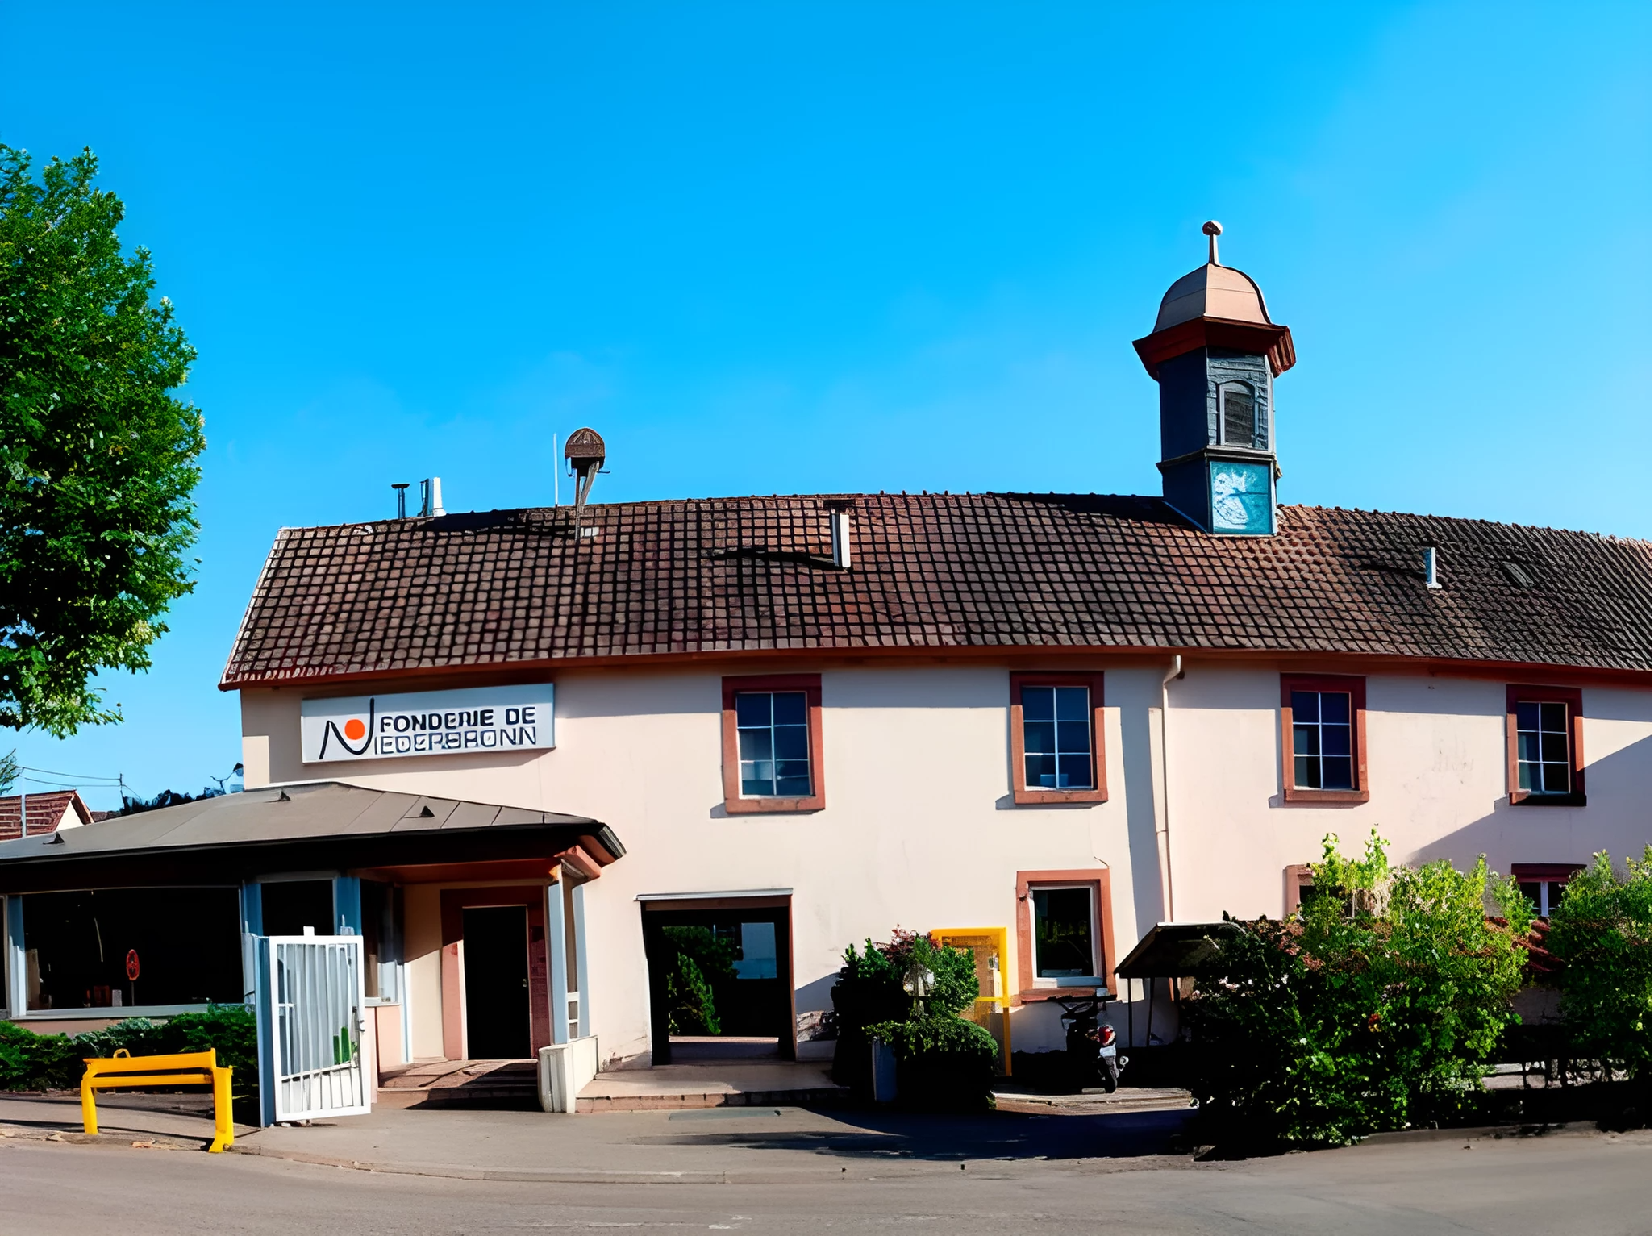
\includegraphics[scale=0.27]{Images/Presentation/Fonderie_vue_de_bas.pdf}
    \hspace{0.5 cm}
    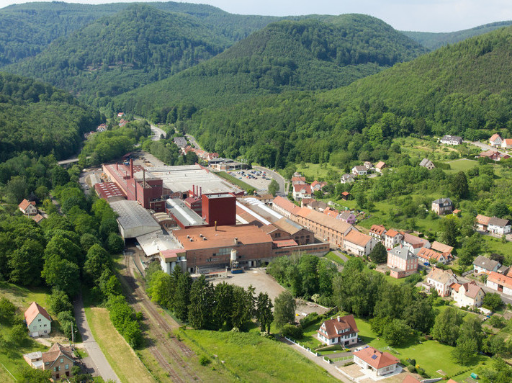
\includegraphics[scale=0.27]{Images/Presentation/Fonderie_vue_de_haut.pdf}
    \caption{Vues extérieure et aérienne de la Fonderie de Niederbronn}
\end{figure}

\newpage

% \subsection{Description du processus de production des pièces en fonte}
\subsection{Description du processus de production}

La production de pièces en fonte suit un processus ordonnée et méticuleux, 
composé de plusieurs étapes interconnectées qui garantissent la qualité 
et la durabilité des produits finis. Chaque étape, depuis la préparation 
des matériaux jusqu'au produit final, est cruciale pour obtenir des pièces 
répondant aux exigences techniques et aux normes industrielles. 
Le schéma ci-dessous illustre ce flux de production, offrant une vue 
d'ensemble des différentes phases. 

\begin{figure}[H]
    \centering
    \begin{adjustbox}{width=1.3\textwidth,height=0.8\textheight,center}
        \includegraphics{Images/Presentation/Flux de production.pdf}
    \end{adjustbox}
    \caption{Flux de production des pièces en fonte.}
    \label{fig:flux-production}
\end{figure}


\begin{enumerate}
    \item \textbf{Modelage :} 
    Le modélage est l'une des premières étapes de la production en fonderie.
    Il consiste à préparer le modèle pour la coulée.
    La pièce finale est d'abord conçue numériquement à l'aide de logiciels 
    de CAO. Une fois la conception validée, un modèle physique est fabriqué
    en métal.

    \item \textbf{Noyautage :} 
    Le noyautage constitue une étape importante dans le processus de 
    fabrication des pièces moulées, notamment pour créer des formes 
    internes complexes ou des cavités spécifiques. Semblables au moule, 
    les noyaux sont souvent réalisés en sable et façonnés à l'aide de 
    boîtes à noyaux qui leur confèrent la géométrie requise. Ces noyaux 
    jouent un rôle déterminant en permettant la formation de canaux et 
    d'autres détails internes indispensables à la pièce finale. 
    Une fois confectionnés, ils sont positionnés avec précision dans 
    le moule, où ils doivent être solidement fixés afin d'éviter 
    tout déplacement pendant la coulée.

    \item \textbf{Chargement des matières premières :}
    Cette étape consiste à préparer les matériaux de base nécessaires 
    à la production de la fonte, tels que le cuivre et les déchets 
    métalliques provenant d'autres industries. Le choix des matériaux 
    est crucial, car leur composition chimique influence directement 
    les propriétés mécaniques de la fonte. Une sélection est donc effectuée
    pour s'assurer que certains éléments chimiques ne compromettent pas 
    la qualité du produit final.


    Voici une illustration des matières premières utilisées dans la fonderie :

    \begin{figure}[H]
        \centering
        \vfill
        \hspace{0.8 cm}
        \includegraphics[scale=0.7]{Images/Presentation/Les Retours.pdf}
        \hspace{0.5 cm}
        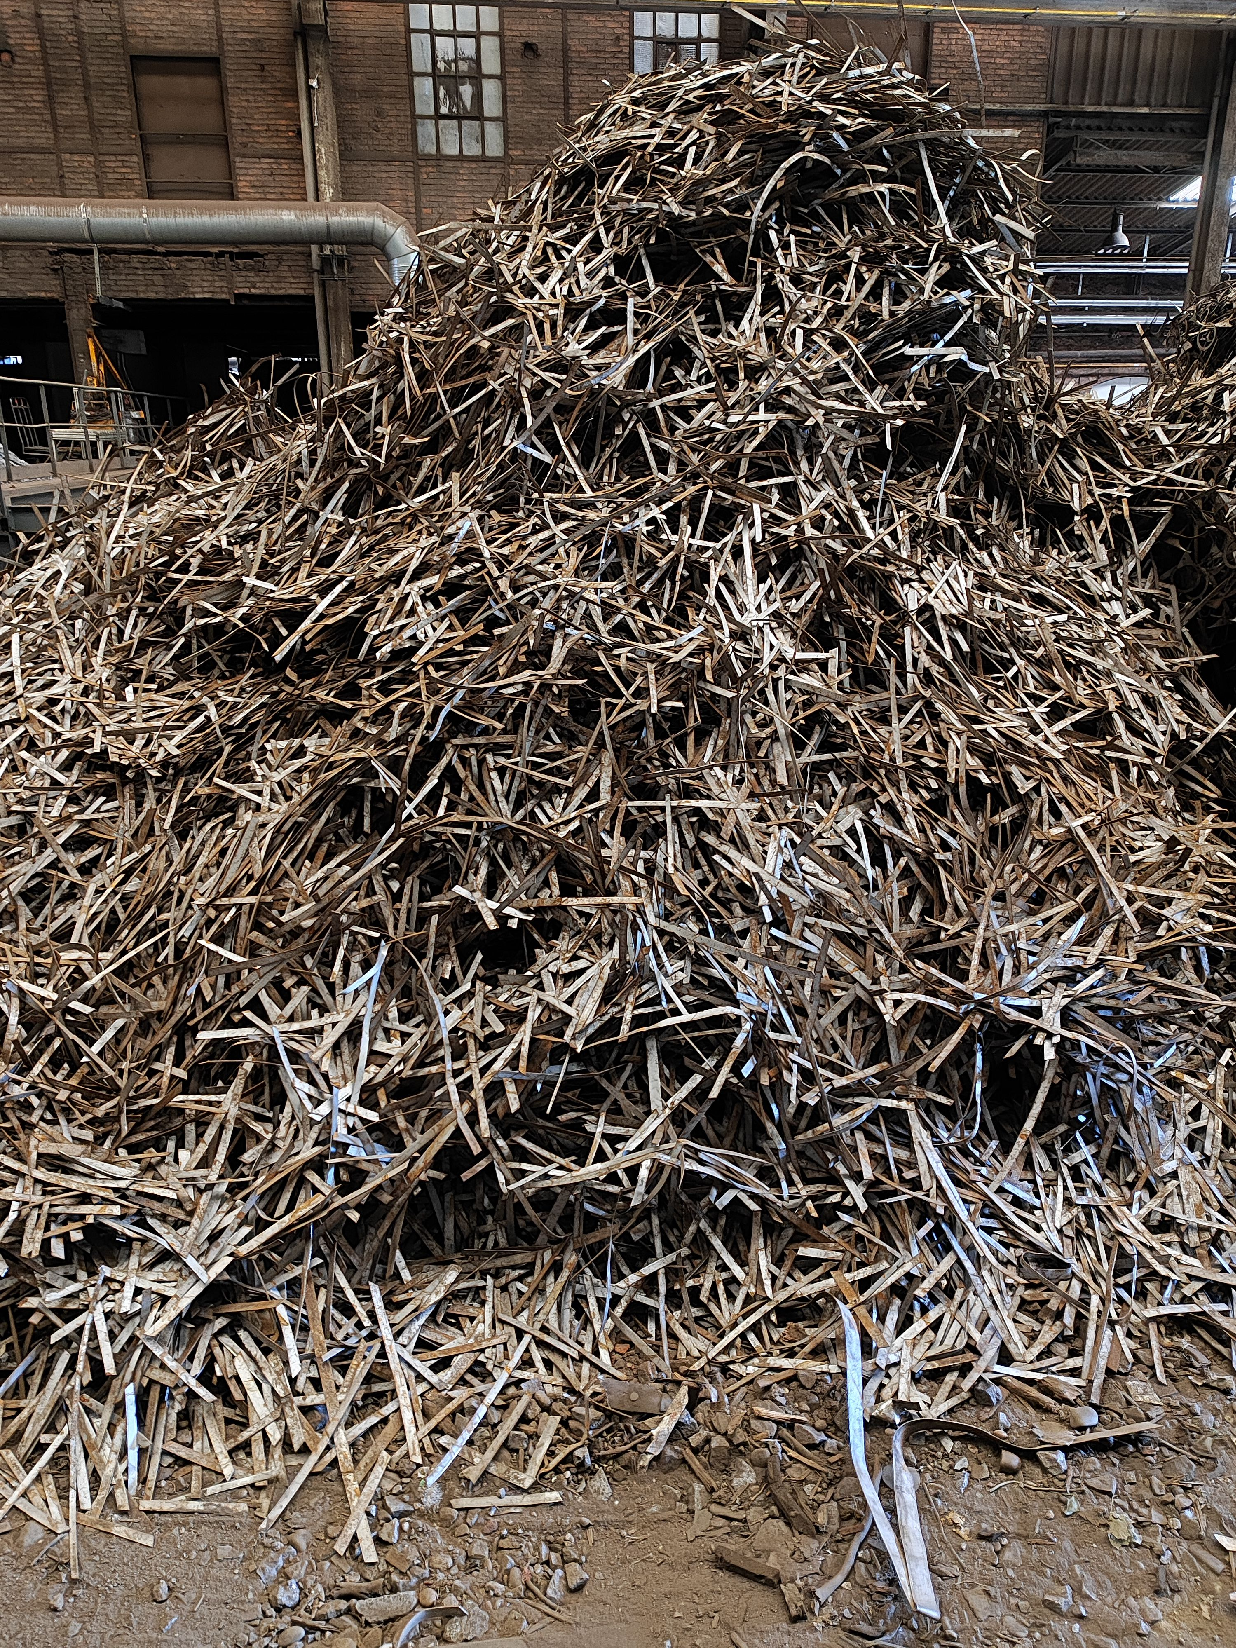
\includegraphics[scale=0.7]{Images/Presentation/Frite Haut Silicium.pdf}
        \caption{Les retours et les Frite Haut Silicium}
    \end{figure}

    \begin{figure}[H]
        \centering
        \vfill
        \hspace{0.8 cm}
        \includegraphics[scale=0.7]{Images/Presentation/Fontes d'affinages.pdf}
        \hspace{0.5 cm}
        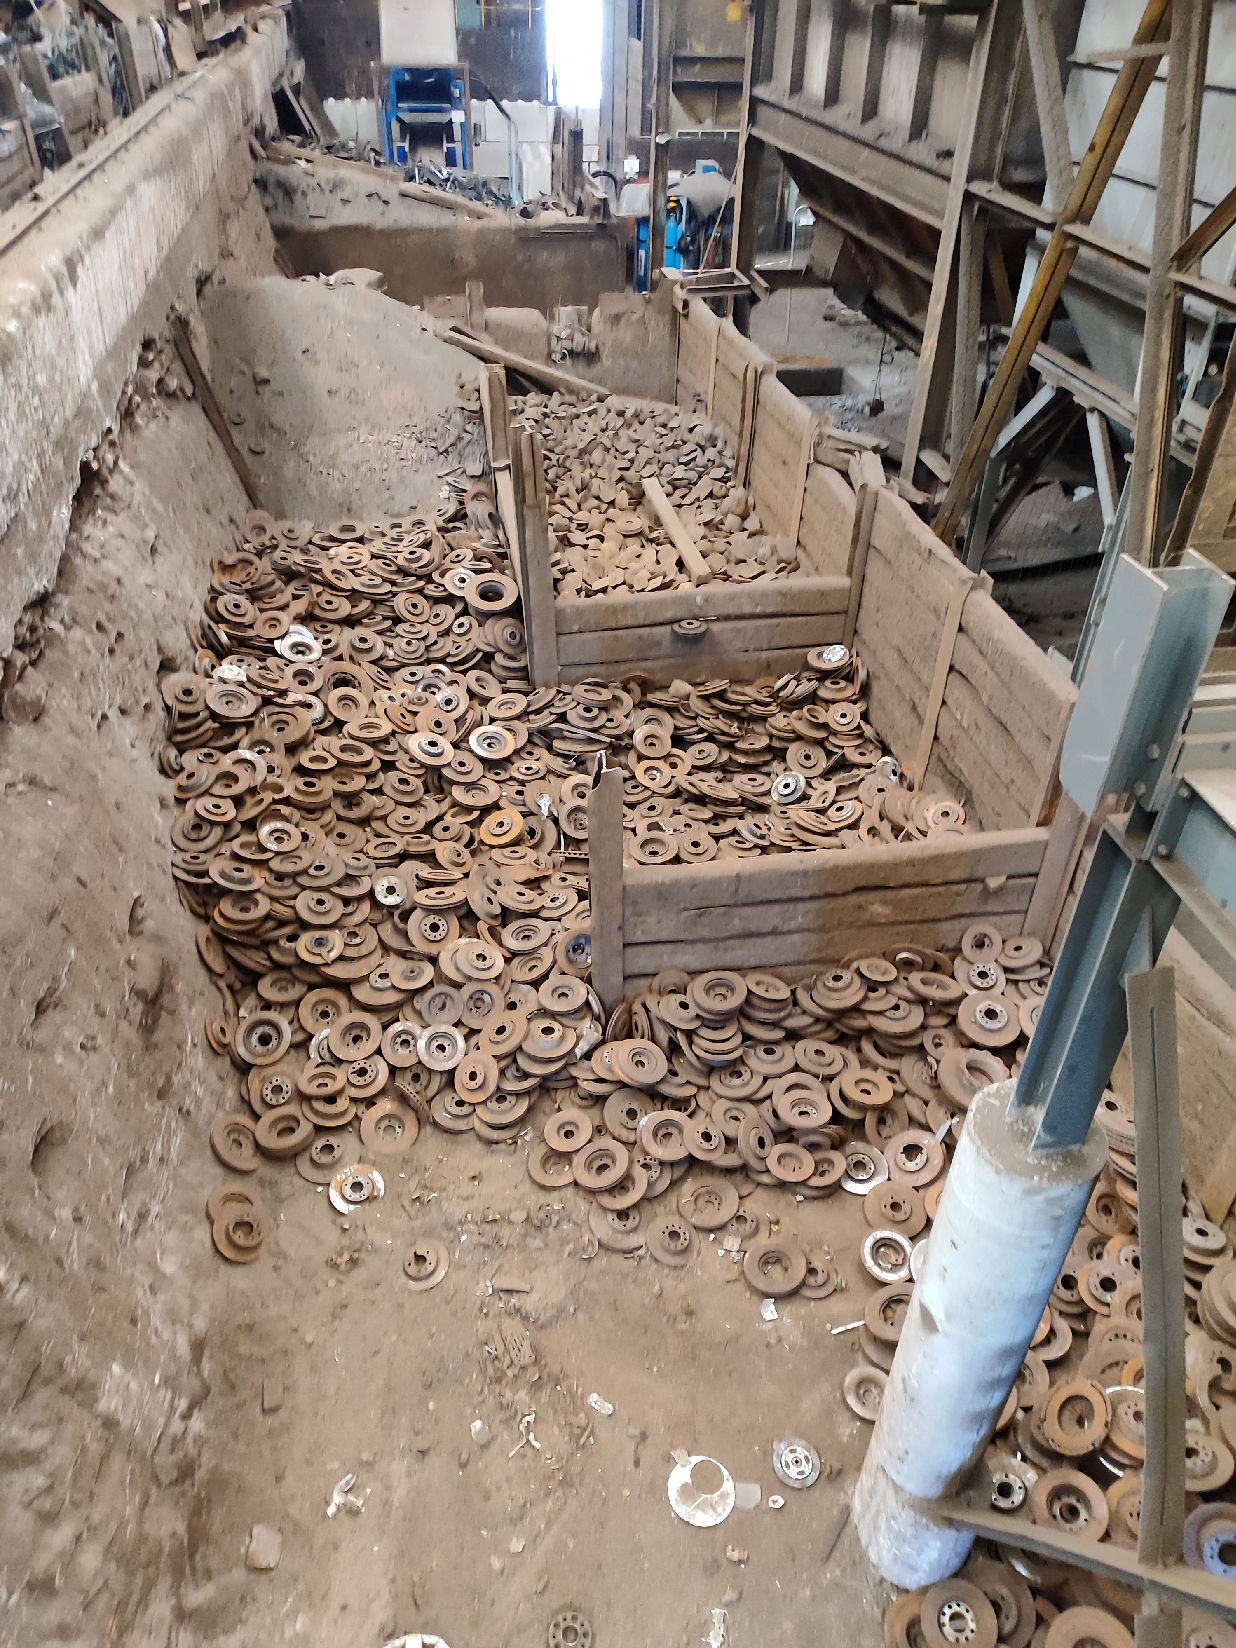
\includegraphics[scale=0.7]{Images/Presentation/Disque.pdf}
        \caption{Les Fontes d'affinages et les Disques}
    \end{figure}


    \item \textbf{Fusion :} Après la sélection des métaux, ceux-ci sont 
    fondus dans un four à induction qui atteint des températures 
    (environ 1500 degrés Celsius) suffisamment élevées pour les transformer
    en métal liquide.


    \item \textbf{Moulage:} 
    Le moule, généralement réalisé en sable mélangé à de l'argile et de 
    l'eau, est compacté autour du modèle. Le sable doit être suffisamment 
    résistant pour supporter le poids du métal fondu sans se désagréger. 
    Après compactage, le modèle est retiré et les parties du moule sont 
    assemblées. Des conduits de coulée sont ensuite ajoutés pour permettre 
    au métal fondu de remplir la cavité du moule.

    % ----------------- Mettre image de modèle physique ?!




    \item \textbf{Sphéroïdisation :} 
    Cette étape est spécifiquement dédiée aux fontes à graphite sphéroïdal 
    (fonte GS). La sphéroïdisation est un procédé essentiel visant à 
    optimiser les propriétés mécaniques de la fonte, en particulier sa 
    ductilité et sa résistance à la traction. Ce processus repose sur 
    l’ajout de magnésium à la fonte liquide, favorisant ainsi la formation 
    de graphite sous forme sphéroïdale plutôt que lamellaire. L'ajout de 
    magnésium se fait souvent à travers un alliage, tel que le fil fourré. 
    Cette transformation microstructurelle, en remplaçant les lamelles de 
    graphite par des sphéroïdes, permet d'améliorer significativement les 
    performances mécaniques et la durabilité de la fonte, la rendant ainsi 
    plus adaptée aux applications exigeantes.


    % ----------------- Mettre image Microscopique de la fonte GS

    \item \textbf{Inoculation et Décrassage :} L'inoculation garantit une 
    précipitation homogène et fine du graphite, minimisant ainsi les 
    défauts structurels. Cette étape est cruciale pour obtenir une 
    distribution optimale du graphite sphéroïdal, améliorant ainsi les 
    performances mécaniques de la pièce.

    Le décrassage, quant à lui, consiste à éliminer les impuretés 
    superficielles. Cette opération est indispensable pour maintenir la 
    pureté du métal et éviter tout défaut dans les pièces finies, 
    garantissant ainsi une coulée propre et de haute qualité.

    % ----------------- Mettre image Innoculation/Degrassange en action ou du produits innoculant
    
    \item \textbf{ Coulée :} La coulée est l'étape où la fonte liquide, 
    préparée et traitée lors des phases précédentes, est soigneusement 
    versée dans le moule à travers un système de conduits conçu pour 
    guider le métal dans toutes les parties de la cavité. Ce processus est
    crucial, car il détermine la répartition uniforme du métal dans le 
    moule, assurant ainsi une formation correcte et homogène de la pièce.

    Une fois le métal versé, il commence à refroidir progressivement, 
    entraînant sa solidification à l'intérieur du moule. Pendant cette 
    phase, le métal adopte la forme précise de la cavité, qui a été 
    façonnée par le modèle et complétée par les noyaux pour former les 
    détails internes complexes. Le contrôle du refroidissement est 
    essentiel, car une solidification trop rapide ou inégale peut 
    entraîner des tensions internes ou des défauts structurels. 
    Ainsi, cette étape marque le point de transition du métal liquide à 
    l'état solide, donnant naissance à la pièce brute.
    
    

    \item \textbf{Décochage et Grenaillage :} Après la solidification 
    complète du métal, le moule est démonté pour extraire la pièce coulée. 
    Cette opération implique souvent la destruction du moule. Les noyaux 
    en sable, utilisés pour créer les cavités internes de la pièce, sont 
    retirés par des procédés mécaniques tels que des vibrations ou des chocs.

    Une fois la pièce extraite, elle subit un processus de grenaillage, 
    qui consiste à projeter des billes d'acier ou d'autres matériaux 
    abrasifs à haute vitesse sur sa surface. Cette étape a pour objectif 
    de nettoyer la pièce en éliminant les résidus de sable et autres 
    impuretés qui se sont formées durant la coulée. 
    
    \item \textbf{Ébarbage et Usinage :} Après le démoulage, la pièce 
    brute nécessite encore d'autres opérations de finition. Le processus 
    d'ébarbage consiste à éliminer les bavures, ou les métaux 
    indésirables qui se forment le long des lignes de joint du moule ou 
    au niveau des conduits de coulée. 

    Une fois ébarbée, la pièce peut passer à l'usinage, une opération plus 
    précise qui vise à atteindre les dimensions désirées. L'usinage permet 
    également d'améliorer la qualité de surface en la rendant plus lisse 
    et conforme aux exigences fonctionnelles de la pièce. 

    \item \textbf{Peinture :} La peinture est appliquée sur la pièce pour 
    assurer à la fois une protection contre la corrosion et un aspect 
    esthétique. Avant l'application de la peinture, la surface de la pièce 
    doit être soigneusement nettoyée et préparée afin de garantir une 
    adhérence optimale du revêtement. Une fois la surface préparée, la 
    peinture est appliquée par pulvérisation, trempage, ou encore au 
    pinceau.

    \item \textbf{Contrôle qualité et Livraison :} Avant la livraison des 
    pièces finales, un contrôle qualité est effectué pour s'assurer 
    qu'elles répondent aux normes et aux spécifications requises. La 
    composition chimique de la pièce et des tests de traction, de dureté, est analysée pour 
    s'assurer qu'elle correspond aux spécifications du client. 
\end{enumerate}


\subsection{Objectifs}

Ce stage est réalisé dans le cadre d'un projet financé par un crédit 
d'impôt recherche. Son objectif principal est d'optimiser l'utilisation 
des matières premières recyclées dans la production de fonte. Plus 
précisément, le stage vise à développer des méthodes de modélisation puis 
d'automatiser les processus associés au choix et aux quantités des matières
premières utilisées.

Les missions confiées dans ce cadre sont les suivantes :

\begin{itemize}
\item \textbf{Modélisation du système :} Développer des modèles mathématiques pour représenter le système de gestion des matières premières.
\item \textbf{Optimisation des coûts :} Contribuer à réduire les coûts de production en automatisant les processus de sélection et de gestion des matières premières.
\item \textbf{Participer à d'autres problèmes d'optimisation :} Contribuer à d'autres défis liés à l'optimisation des procédés de production de fonte.
\end{itemize}

\subsection{Le plan du rapport}

% % Presenter rapidement le plan du rapport

% Le présent rapport couvre les éléments suivants :  un contexte
% générale qui présentation de la fonderie de Niederbronn, la description du processus 
% de production ; une etude statistique visant à predire la qualité des 
% pièces en fonction de sa composition chimique; on cherchera à 
% la determinatisation de la recette optimale des matières prmeières ;et une derniere partie 
% sphérodisation visant à réduire le cout du fil fourrée et garantir
% le bon fonctionnement de cette étape.En fin une conclusion générale du stage.

 

% Presenter rapidement le plan du rapport

Ce rapport est organisé en plusieurs sections principales. Il débute par 
un contexte général qui présente la Fonderie de Niederbronn et décrit 
son processus de production. La section suivante est dédiée à une étude 
statistique visant à prédire la qualité des pièces en fonction de leur 
composition chimique. Ensuite, une partie du rapport est consacrée à la 
détermination de la recette optimale des matières premières. Cette analyse 
a pour but d'optimiser la sélection et les proportions des matériaux 
utilisés dans la production de fonte. Une autre section du rapport examine 
le processus de sphérodisation, avec pour objectif de réduire les coûts 
de production associés à cette étape et de garantir son bon fonctionnement.
Le rapport se conclut par une synthèse des principaux résultats et 
enseignements tirés du stage.




%---- motiver le sujet et objectif stage


%---- détail objectif stage





\section{L'étude statistique}

% Contexte et Objectifs

\subsection{Contexte et Objectifs}

Au sein de la fonderie, deux mesures normatives sont utilisées pour évaluer 
les propriétés mécaniques de la fonte : la résistance mécanique, exprimée 
en MPa (mégapascals), et l'allongement, exprimé en pourcentage. La 
résistance mécanique mesure la capacité de la fonte à résister à une 
force ou à une contrainte avant de se rompre. Exprimée en mégapascals (MPa), 
cette valeur indique la force maximale que le matériau peut supporter par 
unité de surface. Ainsi une résistance mécanique élevée signifie que la 
pièce en fonte pourra supporter des charges importantes sans se casser.
L'allongement est une mesure de la capacité du matériau à se déformer sous 
tension avant de se rompre. Il est exprimé en pourcentage et indique à 
quel point la pièce peut s'étirer avant de casser. Un allongement plus 
élevé signifie que le matériau est plus ductile, c'est-à-dire capable de 
se déformer sans se briser. 

En complément de ces deux mesures normatives, 
des analyses de la composition chimique de la fonte sont également 
réalisées. A partir de cette composition chimique, des indicateurs de 
qualité sont calculés par des combinaisons linéaire de ses éléments 
chimiques.

Voici les principales formules proposées par 
différents auteurs pour essayer d'apprécier l'action globale de ces divers 
éléments soit sur la matrice, soit sur la forme du graphite.


% --------- 1

\textbf{1} L’indice d’impureté I, proposé par S. PARENT-SIMONIN et 
J.C. MARGERIE, est un indicateur utilisé pour prédire la structure 
d'une fonte après moulage. Ce modèle tient compte de la classe de la 
fonte, notamment de sa teneur en silicium, un élément crucial influençant 
sa solidification.

L'idée principale derrière cet indice est de déterminer la qualité de 
la fonte après un processus de refusion, c'est-à-dire après que 
la fonte a été refondue dans des conditions spécifiques.

 
\begin{align*}
    \textcolor{purple}{\text{Impureté \%}} &= 4.9 (\text{Cu \%}) + 0.37 (\text{Ni \%}) + 0.37 (\text{Cr \%}) + 7.9 (\text{Mo \%}) + 4.4 (\text{Ti \%})\\
    &\quad + 39.0 (\text{Sn \%}) + 0.44 (\text{Mn \%}) + 5.6 (\text{P \%})
\end{align*}


% --------- 2

\textbf{2} Dans les fontes à graphite sphéroïdal à l’état brut de 
coulée, MOTZ et ORTHS proposent une formule de régression donnant le 
pourcentage de ferrite en fonction de certains éléments présents :


\begin{align*}
    \textcolor{red}{\text{Ferrite \%}} &= 92.3 - 96.2 (\text{Mn \%}) - 211 (\text{Cu \%}) - 14270 (\text{Pb \%}) - 2815 (\text{Sb \%})
\end{align*}


Il apparaît que le plomb et l’antimoine ont une action prépondérante.


% --------- 3

\textbf{3} Pour K. ONO, H. TANIMURA, K. KODAMA et K. SATO, qui ont 
étudié l’influence des oligo-éléments sur les moulages, la pureté doit 
être la plus grande possible aussi bien pour assurer de hautes 
caractéristiques dans la fonte à graphite lamellaire que pour avoir 
une graphitisation rapide dans la fonte malléable ou bien encore, 
obtenir une sphéricité parfaite du graphite dans les fontes à graphite 
sphéroïdal. Pour cela, ils préconisent que :

\begin{align*}
    \textcolor{green}{\text{Pureté ONO \%}} &= \text{Cu \%} + \text{Ti \%} + \text{Ni \%} + \text{Cr \%} + \text{V \%} + \text{Al \%} + \text{As \%} + \text{Sn \%} \\
    &\quad + \text{Pb \%} + \text{Sb \%} + \text{Bi \%}
\end{align*}

Toutefois une ferrite trop pure, par exemple dans les fontes malléables, 
peut conduire à une basse limite d'élasticité.



% --------- 4
\textbf{4} T. THIELEMANN propose de considérer que la fonte à graphite 
sphéroïdal est pure si l'expression ci-dessous est vérifiée :

\begin{align*}
    \textcolor{orange}{\text{Pureté THIELMANN \%}} &= 4.4 (\text{Ti \%}) + 2.0 (\text{As \%}) + 2.3 (\text{Sn \%}) + 5.0 (\text{Sb \%}) \\
    &\quad + 290 (\text{Pb \%}) + 370 (\text{Bi \%}) + 1.6 (\text{Al \%})
\end{align*}


% --------- 5
\textbf{5} H. MAYER maintient la relation

\begin{align*}
    \textcolor{blue}{\text{Pureté MAYER \%}} &= \text{Ti \%} + \text{Pb \%} + \text{Bi \%} + \text{Sb \%}
\end{align*}

pour que le graphite soit sphéroïdal dans les pièces d’épaisseur supérieure
à 100 mm.


L'objectif principal de cette étude est d'évaluer la pertinence de ces 
cinq indicateurs de qualité par rapport aux deux mesures normatives, et 
d'identifier les meilleurs indicateurs pour prédire les performances 
mécaniques de la fonte. Une fois les meilleurs indicateurs sélectionnés, 
nous déterminerons leurs intervalles de prédiction, ce qui permettra 
d'anticiper les performances de la fonte en fonction de sa composition 
chimique.









\subsection{Les données}

% Source  et Format des données 
Les données utilisées dans cette étude proviennent de deux instruments 
de mesure principaux. La résistance mécanique et l'allongement des 
échantillons de fonte sont mesurés à l'aide d'une machine de traction. 
Cette machine permet de déterminer la capacité du matériau à supporter 
des forces et sa ductilité sous contrainte. En parallèle, la composition chimique des échantillons est analysée à 
l'aide d'un spectromètre. Cet appareil fournit des informations détaillées 
sur la concentration des différents éléments chimiques présents dans la 
fonte. Les données utilisees sont ensuite exportées sous forme de fichiers 
Excel, à partir du logiciel Windev. Les données peuvent être regroupées 
en plusieurs catégories : les variables quantitatives, les indicateurs 
de qualité, les variables qualitatives, et les éléments chimiques, pour 
un total de 38 caractéristiques.

% Description des données
\vspace{0.5cm}

\textbf{Les variables quantitatives :}

\begin{itemize}
\item[$\bullet$] Rm : Résistance mécanique à la traction.
\item[$\bullet$] Rp0.2 : Limite d'élasticité à 0,2\% de déformation.
\item[$\bullet$] A\% : Allongement à la rupture en pourcentage.
\item[$\bullet$] Contre-essai A\% : Contre-essai de l'allongement à la rupture en pourcentage.
\item[$\bullet$] Moyenne allongement : Moyenne de l'allongement à la rupture en pourcentage.
\end{itemize}
    
\vspace{0.5cm}

\textbf{Les indicateurs :}

\begin{itemize}
\item[$\bullet$] Impureté : Pourcentage d'impureté dans l'échantillon.
\item[$\bullet$] \% Ferrite : Pourcentage de ferrite dans l'échantillon.
\item[$\bullet$] ONO, TANIMURA, ... : Un indicateur de qualité en pourcentage.
\item[$\bullet$] THIELMANN : Un indicateur de qualité en pourcentage.
\end{itemize}
 
\vspace{0.5cm}

\textbf{Les variables qualitatives :}

\begin{itemize}
\item[$\bullet$] Recette : Nom ou code de la recette associée à l'échantillon.
\item[$\bullet$] Date : Date à laquelle la coulée a été effectuée.
\item[$\bullet$] Poche/Four/Barreau : Indication sur la provenance de l'échantillon (poche, four, barreau, etc.).
\item[$\bullet$] Conforme ? : Indique si l'échantillon est conforme (1) ou non conforme (0) aux critères définis.
\item[$\bullet$] Pièces : Référence des pièces.
\item[$\bullet$] Observations : Commentaires ou observations sur l'échantillon.
\item[$\bullet$] Comment. RQ : Commentaires ou remarques supplémentaires du responsable qualité.
\end{itemize}

\vspace{0.5cm}

\textbf{Les éléments chimiques :}

\begin{itemize}
\item[$\bullet$] C, Si, Mn, P, Cr, Mo, Cu, Sn, Mg, Ce, Ca, Al 
\item[$\bullet$] Zn, Ti, S, Sn, V, Pb, Al, Bi, B, Te, Sb, As, Ti 
\end{itemize}


Selon la littérature, on classe les éléments chimiques en plusieurs catégories :
\begin{itemize}
    \item \textbf{Les éléments d'alliage :}  C, Si, Mn, P, Cr, Mo, Cu, Sn 
    \item \textbf{Les éléments de traitement :} Mg, Ce, Ca, Al
    \item \textbf{Les éléments polluants :}  Zn, Ti, S, Sn, V 
    \item \textbf{Les éléments poisons :}  Pb, Al, Bi, B, Te, Sb, As, Ti
\end{itemize}




En 2024, 209 données ont été collectées, et 308 en 2023, pour un total de 
517 données. La fonderie produit quatre nuances de fontes GS : GS 600-3, 
GS 450-10, GS 500-7, et GS 400-15. Les données collectées se répartissent 
ainsi : 10 pour la GS 400-15, 92 pour la GS 450-10, 29 pour la GS 500-7, 
et 45 pour la GS 600-3. En raison du nombre limité de données disponibles 
pour certaines nuances, l'étude statistique se concentrera exclusivement 
sur la GS 450-10.





La Figure ci-dessous ~\ref{fig:donnees_brutes}  illustre l'état initial des données avant tout 
processus de nettoyage ou d'analyse.


% Les données brutes
\begin{figure}[H]
    \centering
    \adjustbox{width=1.23\textwidth, center}{
        \begin{minipage}{\textwidth}
            \centering
            \includegraphics[width=0.75\paperwidth]{Images/Statistique/DonnéesBrut1.pdf} \\
            \vspace{25pt}
            \includegraphics[width=0.75\paperwidth]{Images/Statistique/DonnéesBrut2.pdf} \\
            \vspace{25pt}
            \includegraphics[width=0.75\paperwidth]{Images/Statistique/DonnéesBrut3.pdf}
        \end{minipage}
    }
    \caption{Visualisation des données brutes}
    \label{fig:donnees_brutes}
\end{figure}





% Prétraitement des Données
Avant d'utiliser les données pour l'analyse, plusieurs étapes de 
prétraitement ont été réalisées pour garantir leur qualité et leur 
pertinence. Voici les principales opérations effectuées :

\begin{itemize}
    \item \textbf{Nettoyage des données} :
    \begin{itemize}
        \item Suppression des colonnes non pertinentes : Date, Rp0.2, A\%, Contre-essai A\%, Pièces, Observations, Comment. RQ, PJ, Ca, Ba.
        \item Élimination des lignes incomplètes contenant des valeurs manquantes.
    \end{itemize}

    \vspace{0.5cm}

    
    \item \textbf{Ajout d'indicateurs} :
    \begin{itemize}
        \item Introduction de l'indicateur de Pureté MAYER pour enrichir les données disponibles.
    \end{itemize}

    
    \vspace{0.5cm}
    
    \item \textbf{Mise en forme des données} :
    \begin{itemize}
        \item Renommage des colonnes pour une meilleure clarté et compréhension.
        \item Segmentation des données en fonction du type de recette pour une analyse plus ciblée.
        \item Classification des données selon la conformité de l'échantillon afin de faciliter les comparaisons.
    \end{itemize}
\end{itemize}

    


% Les données nettoyées
\begin{figure}[H]
    \centering
    \adjustbox{width=1.23\textwidth, center}{
        \begin{minipage}{\textwidth}
            \centering
            \includegraphics[width=\textwidth]{Images/Statistique/DonnéesClean1.pdf} \\
            \vspace{25pt}
            \includegraphics[width=\textwidth]{Images/Statistique/DonnéesClean2.pdf}
        \end{minipage}
    }
    \caption{Visualisation des données nettoyées}
    \label{fig:donnees_nettoyees}
\end{figure}




% \begin{align*}
%     \textcolor{blue}{\text{Pureté MAYER \%}} &= \text{Ti\%} + \text{Pb\%} + \text{Bi\%} + \text{Sb\%} \\
%     \textcolor{red}{\text{Ferrite \%}} &= 92.3 - 96.2 (\text{Mn \%}) - 211 (\text{Cu \%}) - 14270 (\text{Pb \%}) \\
%     &\quad - 2815 (\text{Sb \%}) \\
%     \textcolor{green}{\text{Pureté ONO \%}} &= \text{Cu \%} + \text{Ti \%} + \text{Ni \%} + \text{Cr \%} + \text{V \%} + \text{Al \%} + \text{As \%} \\
%     &\quad + \text{Sn \%} + \text{Pb \%} + \text{Sb \%} + \text{Bi \%} \\
%     \textcolor{purple}{\text{Impureté \%}} &= 4.9 (\text{Cu \%}) + 0.37 (\text{Ni \%}) + 0.37 (\text{Cr \%}) + 7.9 (\text{Mo \%}) \\
%     &\quad + 4.4 (\text{Ti \%}) + 39.0 (\text{Sn \%}) + 0.44 (\text{Mn \%}) + 5.6 (\text{P \%}) \\
%     \textcolor{orange}{\text{Pureté THIELMANN \%}} &= 4.4 (\text{Ti \%}) + 2.0 (\text{As \%}) + 2.3 (\text{Sn \%}) + 5.0 (\text{Sb \%}) \\
%     &\quad + 290 (\text{Pb \%}) + 370 (\text{Bi \%}) + 1.6 (\text{Al \%})
% \end{align*}
    


\subsection{Les indicateurs}

À présent, nous allons évaluer la pertinence des cinq indicateurs de 
qualité à la vue des deux mesures normatives, à savoir l'allongement 
et la résistance mécanique. Pour ce faire, nous utilisons le coefficient de corrélation de Pearson, 
un outil statistique permettant de mesurer la force et la direction de 
la relation linéaire entre deux variables quantitatives. 

Le coefficient de corrélation de Pearson (\( r \)), se calcule 
à partir des covariances des deux variables et des écarts-types respectifs.
Il est défini par la formule suivante :

\[
r = \frac{\text{Cov}(X,Y)}{\sigma_X \sigma_Y}
\]

où :
\begin{itemize}
    \item \(\text{Cov}(X,Y)\) est la covariance des variables \( X \) et \( Y \),
    \item \(\sigma_X\) et \(\sigma_Y\) sont les écarts-types des variables \( X \) et \( Y \).
\end{itemize}

Le coefficient \( r \) prend des valeurs comprises entre -1 et 1 :
\begin{itemize}
    \item Un coefficient proche de 1 indique une forte corrélation positive, c'est-à-dire que lorsque la valeur de l'une des variables augmente, celle de l'autre augmente également de manière proportionnelle.
    \item Un coefficient proche de -1 indique une forte corrélation négative, signifiant qu'une augmentation de la première variable entraîne une diminution proportionnelle de la seconde.
    \item Un coefficient proche de 0 suggère une absence de corrélation linéaire entre les deux variables, indiquant que les variations de l'une ne sont pas prévisibles à partir des variations de l'autre.
\end{itemize}

Après le calcul des coefficients de corrélation de Pearson, l'objectif 
est de classer ces indicateurs.
Pour effectuer ce classement, nous utilisons 
la formule suivante pour établir un score global pour chaque indicateur :

\[
\text{Score} = \frac{|\text{Corrélation avec Rm}| + |\text{Corrélation avec l'Allongement}|}{2}
\]


Une fois ce classement établi, nous conservons uniquement les indicateurs 
présentant la dépendance linéaire la plus forte avec les deux mesures 
normatives. 


% Évaluation des indicateurs 
\begin{figure}[H]
    \includegraphics[width=\textwidth]{Images/Statistique/Matrice_corrélation_qualite_indicateur.pdf} 
    \caption{Corrélation entre les indicateurs et les mesures normatives}
    \label{fig:Corrélation1}
\end{figure}


\begin{center}
    \textbf{Classement des indicateurs :}
    \vspace{0.3cm} % \hspace{2cm} 
    \begin{itemize}
        \item Impureté [\%] : 0.673506
        \item Pureté ONO [\%] : 0.583101
        \item Pureté THIELMANN [\%] : 0.353988
        \item Pureté MAYER [\%] : 0.346637
        \item Ferrite [\%] : 0.327601
    \end{itemize}
\end{center}






L'analyse des corrélations a révélé plusieurs relations importantes. 
Une corrélation positive modérée de 0,65 a été observée entre la résistance
à la traction Rm et l'allongement moyen, indiquant qu'une meilleure 
résistance est associée à une organisation plus homogène des matériaux. 
De même, une corrélation positive de 0,62 entre Rm et la pureté ONO 
suggère que la pureté chimique améliore la résistance mécanique.

En outre, une très forte corrélation positive de 0,86 a été trouvée entre 
l'allongement moyen et la teneur en ferrite, ce qui indique des mécanismes 
communs influençant ces deux variables. Cependant, une corrélation 
négative modérée de -0,41 a été identifiée entre Rm et la ferrite, 
suggérant que des niveaux plus élevés de ferrite diminuent la résistance 
mécanique. Enfin, une corrélation négative de -0,52 entre Rm et la pureté 
THIELMANN montre qu'une pureté plus élevée est liée à une réduction de 
la résistance à la traction. En ce qui concerne les scores, l'impureté 
et la pureté obtiennent les meilleurs résultats, avec des scores de 0,67 
et 0,5 respectivement, et sont donc retenues pour la suite de l'analyse.


\subsection{Les éléments chimiques}


%  Les éléments chimiques

La figure ci-dessous illustre la matrice de corrélation entre l'impureté 
et les éléments chimiques. Cette analyse permet d'identifier les 
variables les plus influentes et d'évaluer leur impact réel sur 
la résistance mécanique et l'allongement des matériaux.




% Impureté
\begin{figure}[H]
    \includegraphics[width=\textwidth]{Images/Statistique/Matrice_corrélation_Impurete_Elements.pdf} 
    \caption{Corrélation entre l'impureté et les éléments chimiques}
    \label{fig:Corrélation2}
\end{figure}


Il existe une forte corrélation positive entre le cuivre (Cu) et 
l'impureté, avec un coefficient de corrélation de 0,75, ainsi 
qu'entre l'étain (Sn) et l'impureté, avec une corrélation de 0,9. 
Par ailleurs, les impuretés présentent une corrélation modérée avec le 
nickel (Ni) (0,36) et le chrome (Cr) (0,52), suggérant également une 
relation positive avec ces éléments. En revanche, les corrélations avec 
les autres éléments chimiques sont faibles et donc peu significatives.






% Purete ONO
\begin{figure}[H]
    \includegraphics[width=\textwidth]{Images/Statistique/Matrice_corrélation_ONO_Elements.pdf} 
    \caption{Corrélation entre la purete ONO et les éléments chimiques}
    \label{fig:Corrélation3}
\end{figure}

La pureté ONO [\%] présente une forte corrélation positive avec le cuivre 
(Cu [\%], 0.93) et le titane (Ti [\%], 0.92), suggérant leur impact majeur 
sur cette pureté. Des corrélations modérées existent avec le nickel 
(Ni [\%], 0.59) et le chrome (Cr [\%], 0.53). En revanche, des éléments 
comme le stibium (Sb [\%]), le bismuth (Bi [\%]), et l’aluminium (Al [\%]) 
montrent des corrélations faibles ou négligeables, indiquant un impact 
limité sur la pureté ONO.





\subsection{Les valeurs extrêmes}

% Gestions des valeurs extrèmes

Avant de procéder à la prédiction de la résistance mécanique et de 
l'allongement de la fonte à partir des mesures d'impureté et de pureté 
ONO, nous éliminons les valeurs extrêmes. Cette étape permet de réduire 
la variabilité des données et d'améliorer la fiabilité de notre modèle 
de régression linéaire.

Une valeur est considérée comme extrême si elle se situe en dehors de 
l'intervalle défini par 
$[\bar{x} - 1.5(Q_3 - Q_1), \bar{x} + 1.5(Q_3 - Q_1)]$, 
où $Q_1$ et $Q_3$, le premier et le troisième quartile 
de la distribution des données, et $\bar{x}$ la moyenne des données.

La suppression des valeurs extrêmes est effectuée de manière itérative 
jusqu'à ce qu'il n'en reste plus dans l'ensemble de données.


Les graphiques suivants illustrent l'effet de ce traitement sur les 
deux principaux indicateurs : l'impureté et la pureté ONO.

% Les valeurs extrèmes de l'impureté
\begin{figure}[H]
    \centering
    \begin{adjustbox}{width=1.3\textwidth,center}
        \includegraphics[scale=1]{Images/Statistique/Impureté_sans_extreme.pdf}
        \includegraphics[scale=1]{Images/Statistique/Impureté_avec_extreme.pdf}
    \end{adjustbox}
    \caption{L'impureté avant et après le traitement des valeurs extrèmes.}
    \label{fig:ExtremeImpurete}
\end{figure}


% Les valeurs extrèmes de ONO
\begin{figure}[H]
    \centering
    \begin{adjustbox}{width=1.3\textwidth,center}
        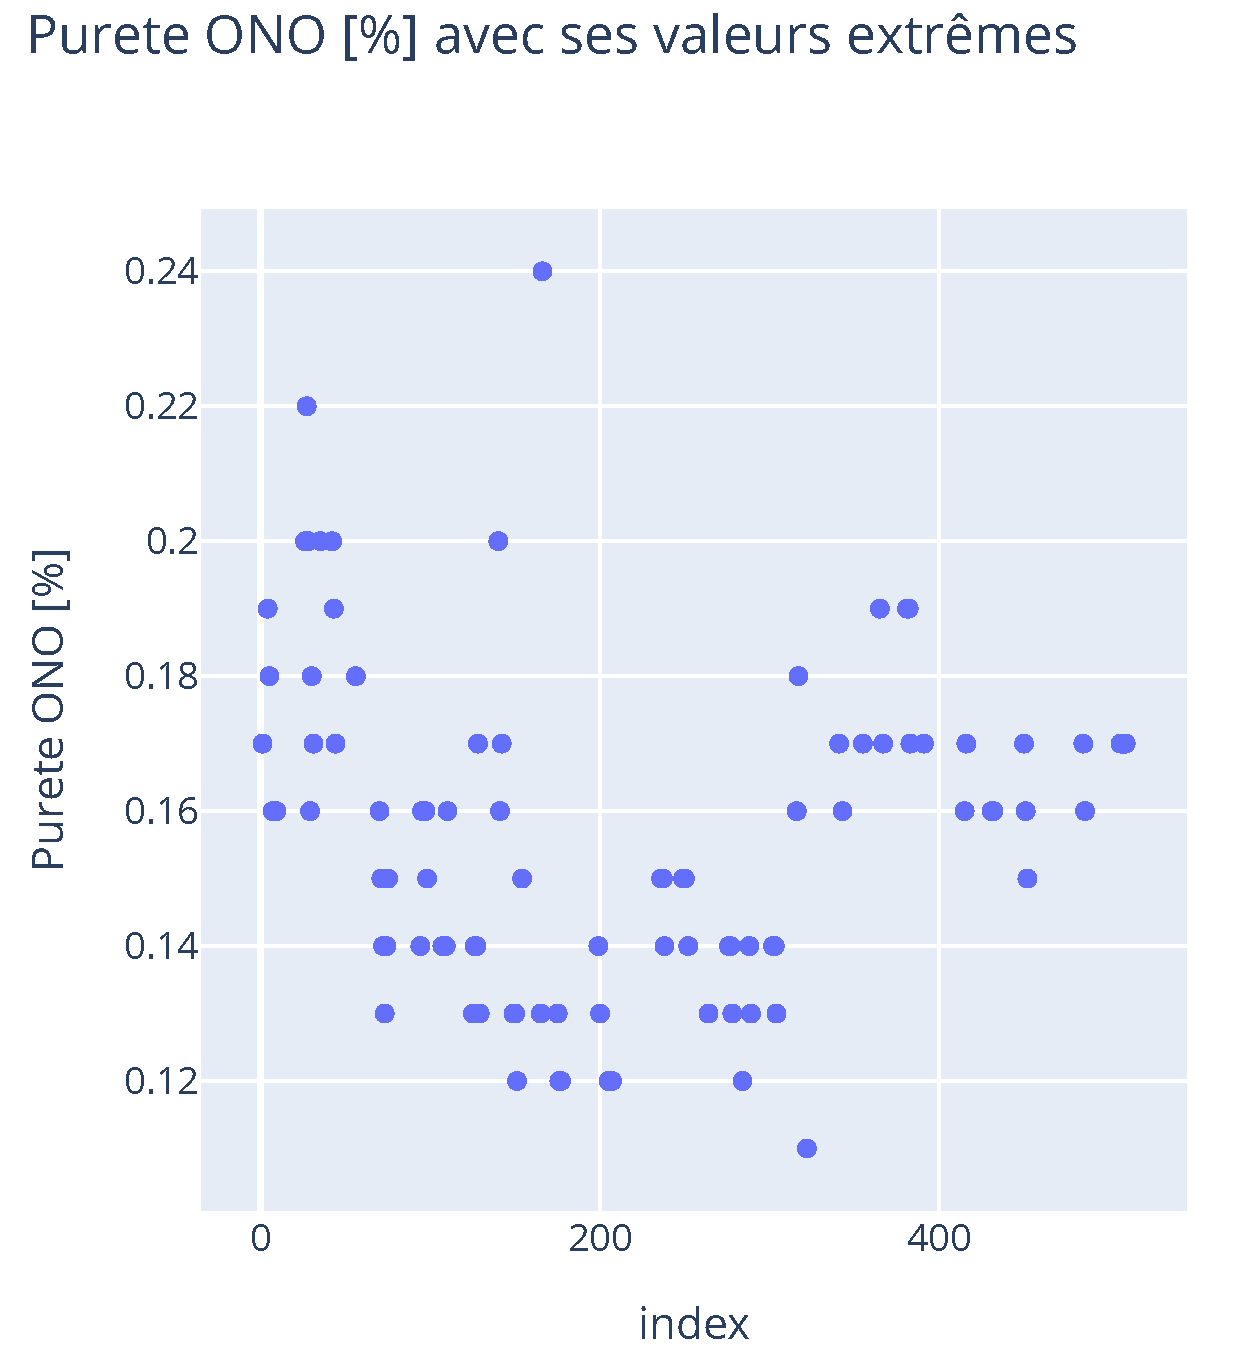
\includegraphics[scale=1]{Images/Statistique/Purete ONO_avec_extreme.pdf}
        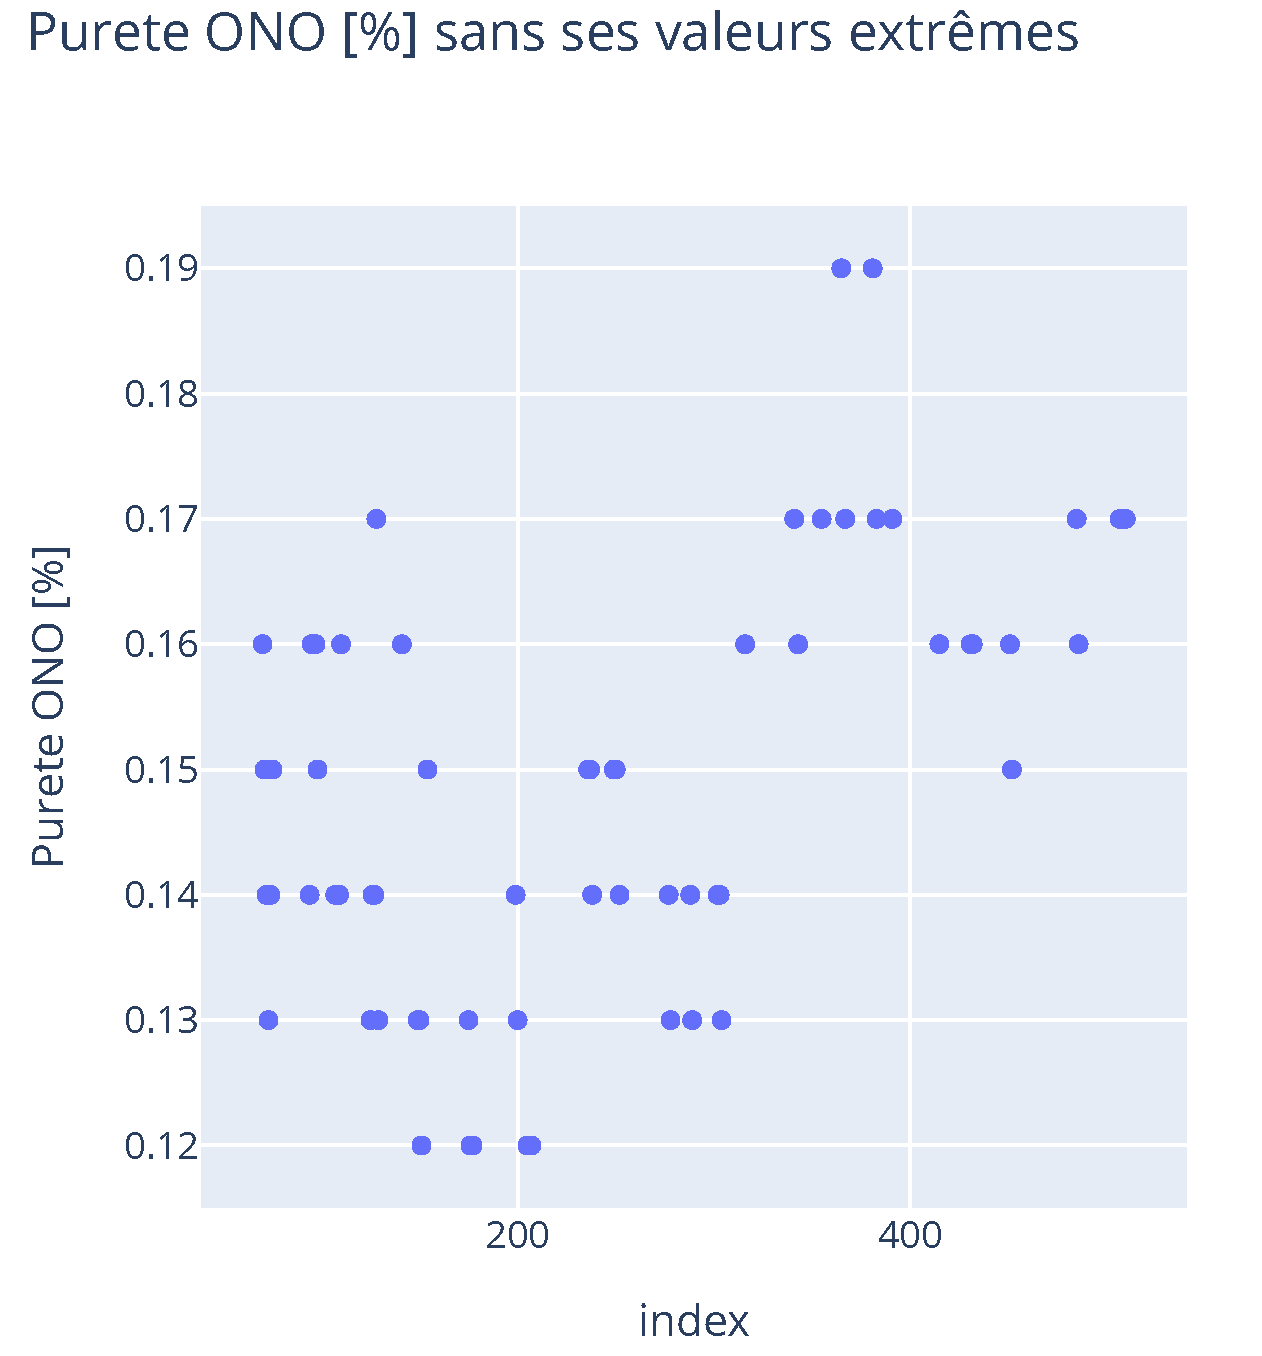
\includegraphics[scale=1]{Images/Statistique/Purete ONO_sans_extreme.pdf}
    \end{adjustbox}
    \caption{La purete ONO avant et après le traitement des valeurs extrèmes.}
    \label{fig:ExtremeONO}
\end{figure}


Les figures \ref{fig:ExtremeImpurete} et \ref{fig:ExtremeONO} 
montrent la réduction de la dispersion des données après 
l'élimination des valeurs extrêmes. Ce traitement rend les distributions 
un peu plus compactes : pour l'impureté, la plage de valeurs passe 
de 0,78-1,91 à 0,93-1,42, tandis que pour la pureté ONO, elle se 
resserre de 0,11-0,24 à 0,12-0,19.

Au total, 28 données ont été supprimées, laissant un ensemble de 
64 données. Bien que ce nettoyage améliore la qualité des données, les 
points restants montrent encore une certaine dispersion. 



% On peut alors discuter des bornes mininum et maximal de l'impurété et de ONO,
% qui permet de garantir un bon lit de fusion.



\subsection{Régression Linéaire}


% La régression linéaire: Analyse des Données

Dans cette section, nous réalisons une régression linéaire pour analyser 
les relations entre certains éléments chimiques et les indicateurs 
pertinents, tels que l'impureté et la pureté ONO. L'objectif est de 
comprendre comment ces variables influencent les 2 indicateurs ainsi que 
les 2 mesures normatives Resistance mecanique et l'allongement, 
et de calculer les intervalles  de confiance et puis l'intervale 
de prédiction pour les valeurs prédites.

\medskip % Ajoute un espace

La formule utilisée pour calculer les intervalles de prédiction est la suivante :
$$
IP (y_{\text{pred}}) = [y_{\text{pred}} - n \cdot \text{predict\_se}, \, y_{\text{pred}} + n \cdot \text{predict\_se}]
$$
où :
\begin{itemize}
    \item $y_{\text{pred}}$ est la valeur prédite par le modèle de 
    régression linéaire.
    \item \text{predict\_se} est l'écart-type associé à la prédiction.
    \item $n$ est un entier naturel qui détermine la largeur de 
    l'intervalle de prédiction.
\end{itemize}


Pour réaliser la régression, la bibliothèque \texttt{statsmodels} de 
Python a été utilisée, en particulier les modules \texttt{sm} pour la 
régression linéaire et \texttt{wls\_prediction\_std} pour l'estimation des 
intervalles de prédiction. De plus, la fonction \texttt{t} de la 
bibliothèque \texttt{scipy.stats} a été employée pour effectuer les 
tests statistiques nécessaires.

Les figures suivantes illustrent les résultats des régressions linéaires 
effectuées. Les relations entre l'impureté et les concentrations des 
éléments chimiques Sn (Étain) et Cu (Cuivre), ainsi qu'entre la pureté 
ONO et les concentrations des éléments Cr (Chrome) et Cu (Cuivre), ont 
d'abord été explorées. Ensuite, les régressions linéaires entre la 
résistance mécanique, l'allongement, et les éléments Sn (Étain), Cr 
(Chrome), et Cu (Cuivre) ont été analysées.

Ces graphiques présentent non seulement les valeurs prédites par les 
modèles de régression, mais aussi les intervalles de prédiction avec 
une largeur de bande fixée à $n=1,5$. 



% Regression linéaire entre Ono et Sn, Cu
% Allongement et Rm

\begin{figure}[H]
    \centering
    \adjustbox{width=1.25\textwidth, center}{  % Ajuste la largeur à la page
        \begin{minipage}{0.8\textwidth}
            \centering
            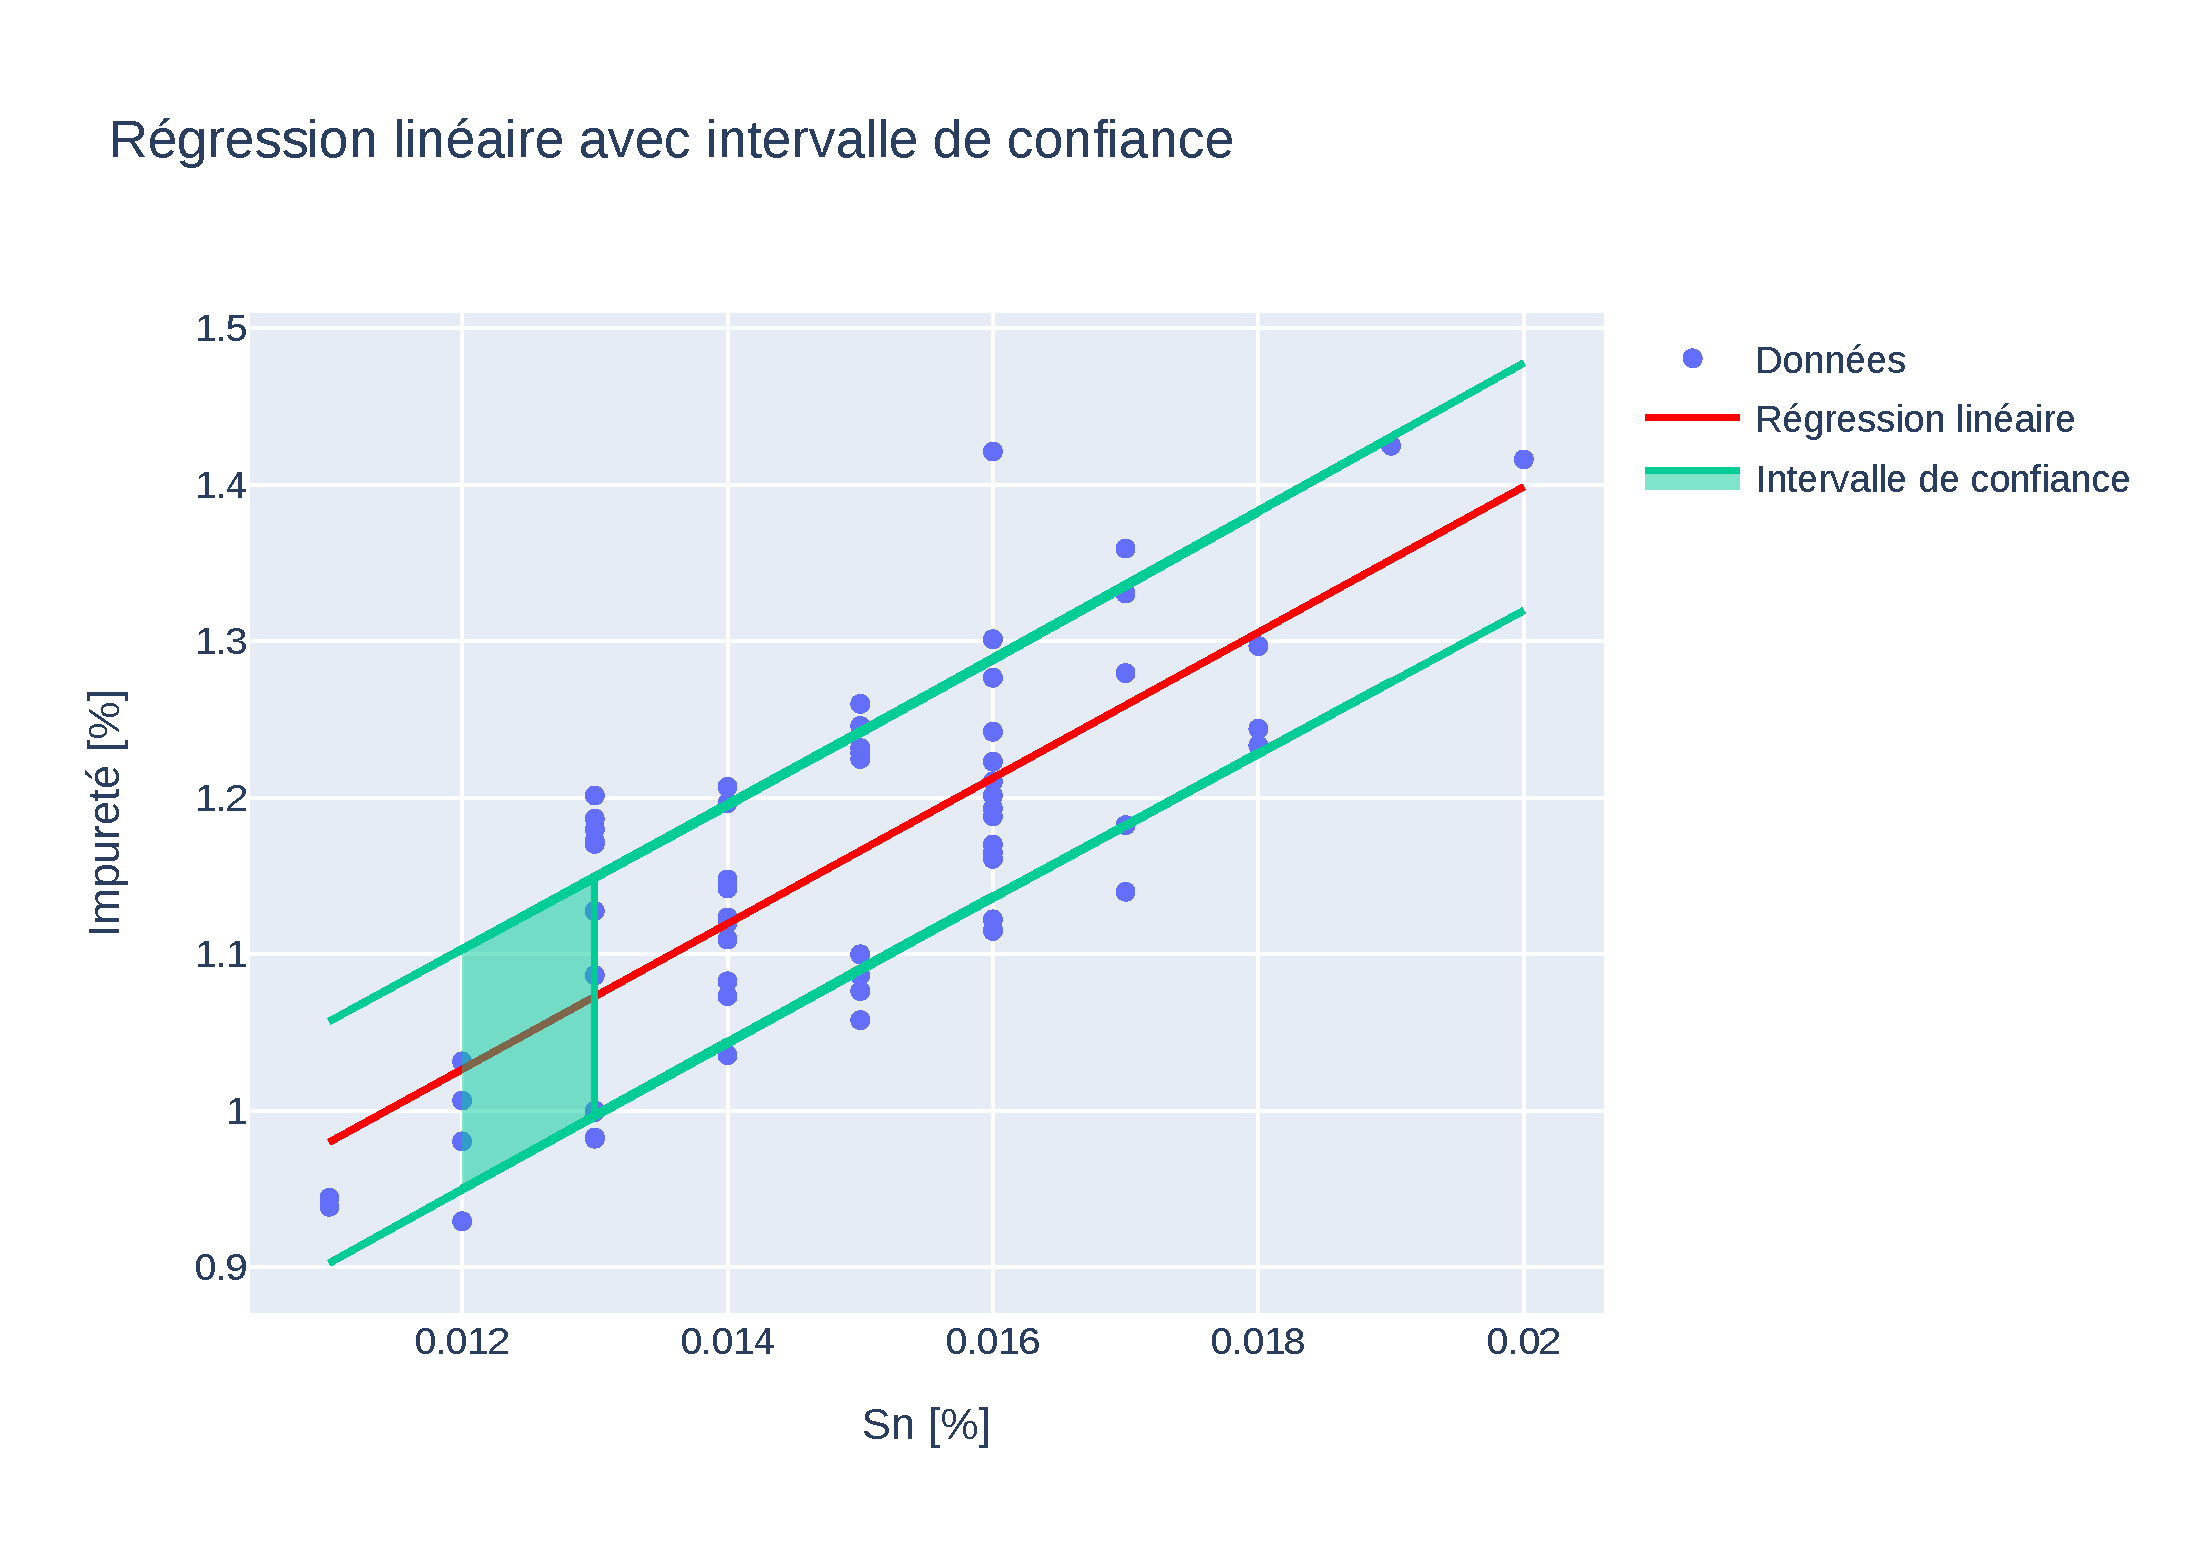
\includegraphics[width=\textwidth]{Images/Statistique/Regression_Impurete_Sn.pdf}
        \end{minipage}
        \hspace{0.01\textwidth}  % Petit espacement entre les colonnes
        \begin{minipage}{0.8\textwidth}
            \centering
            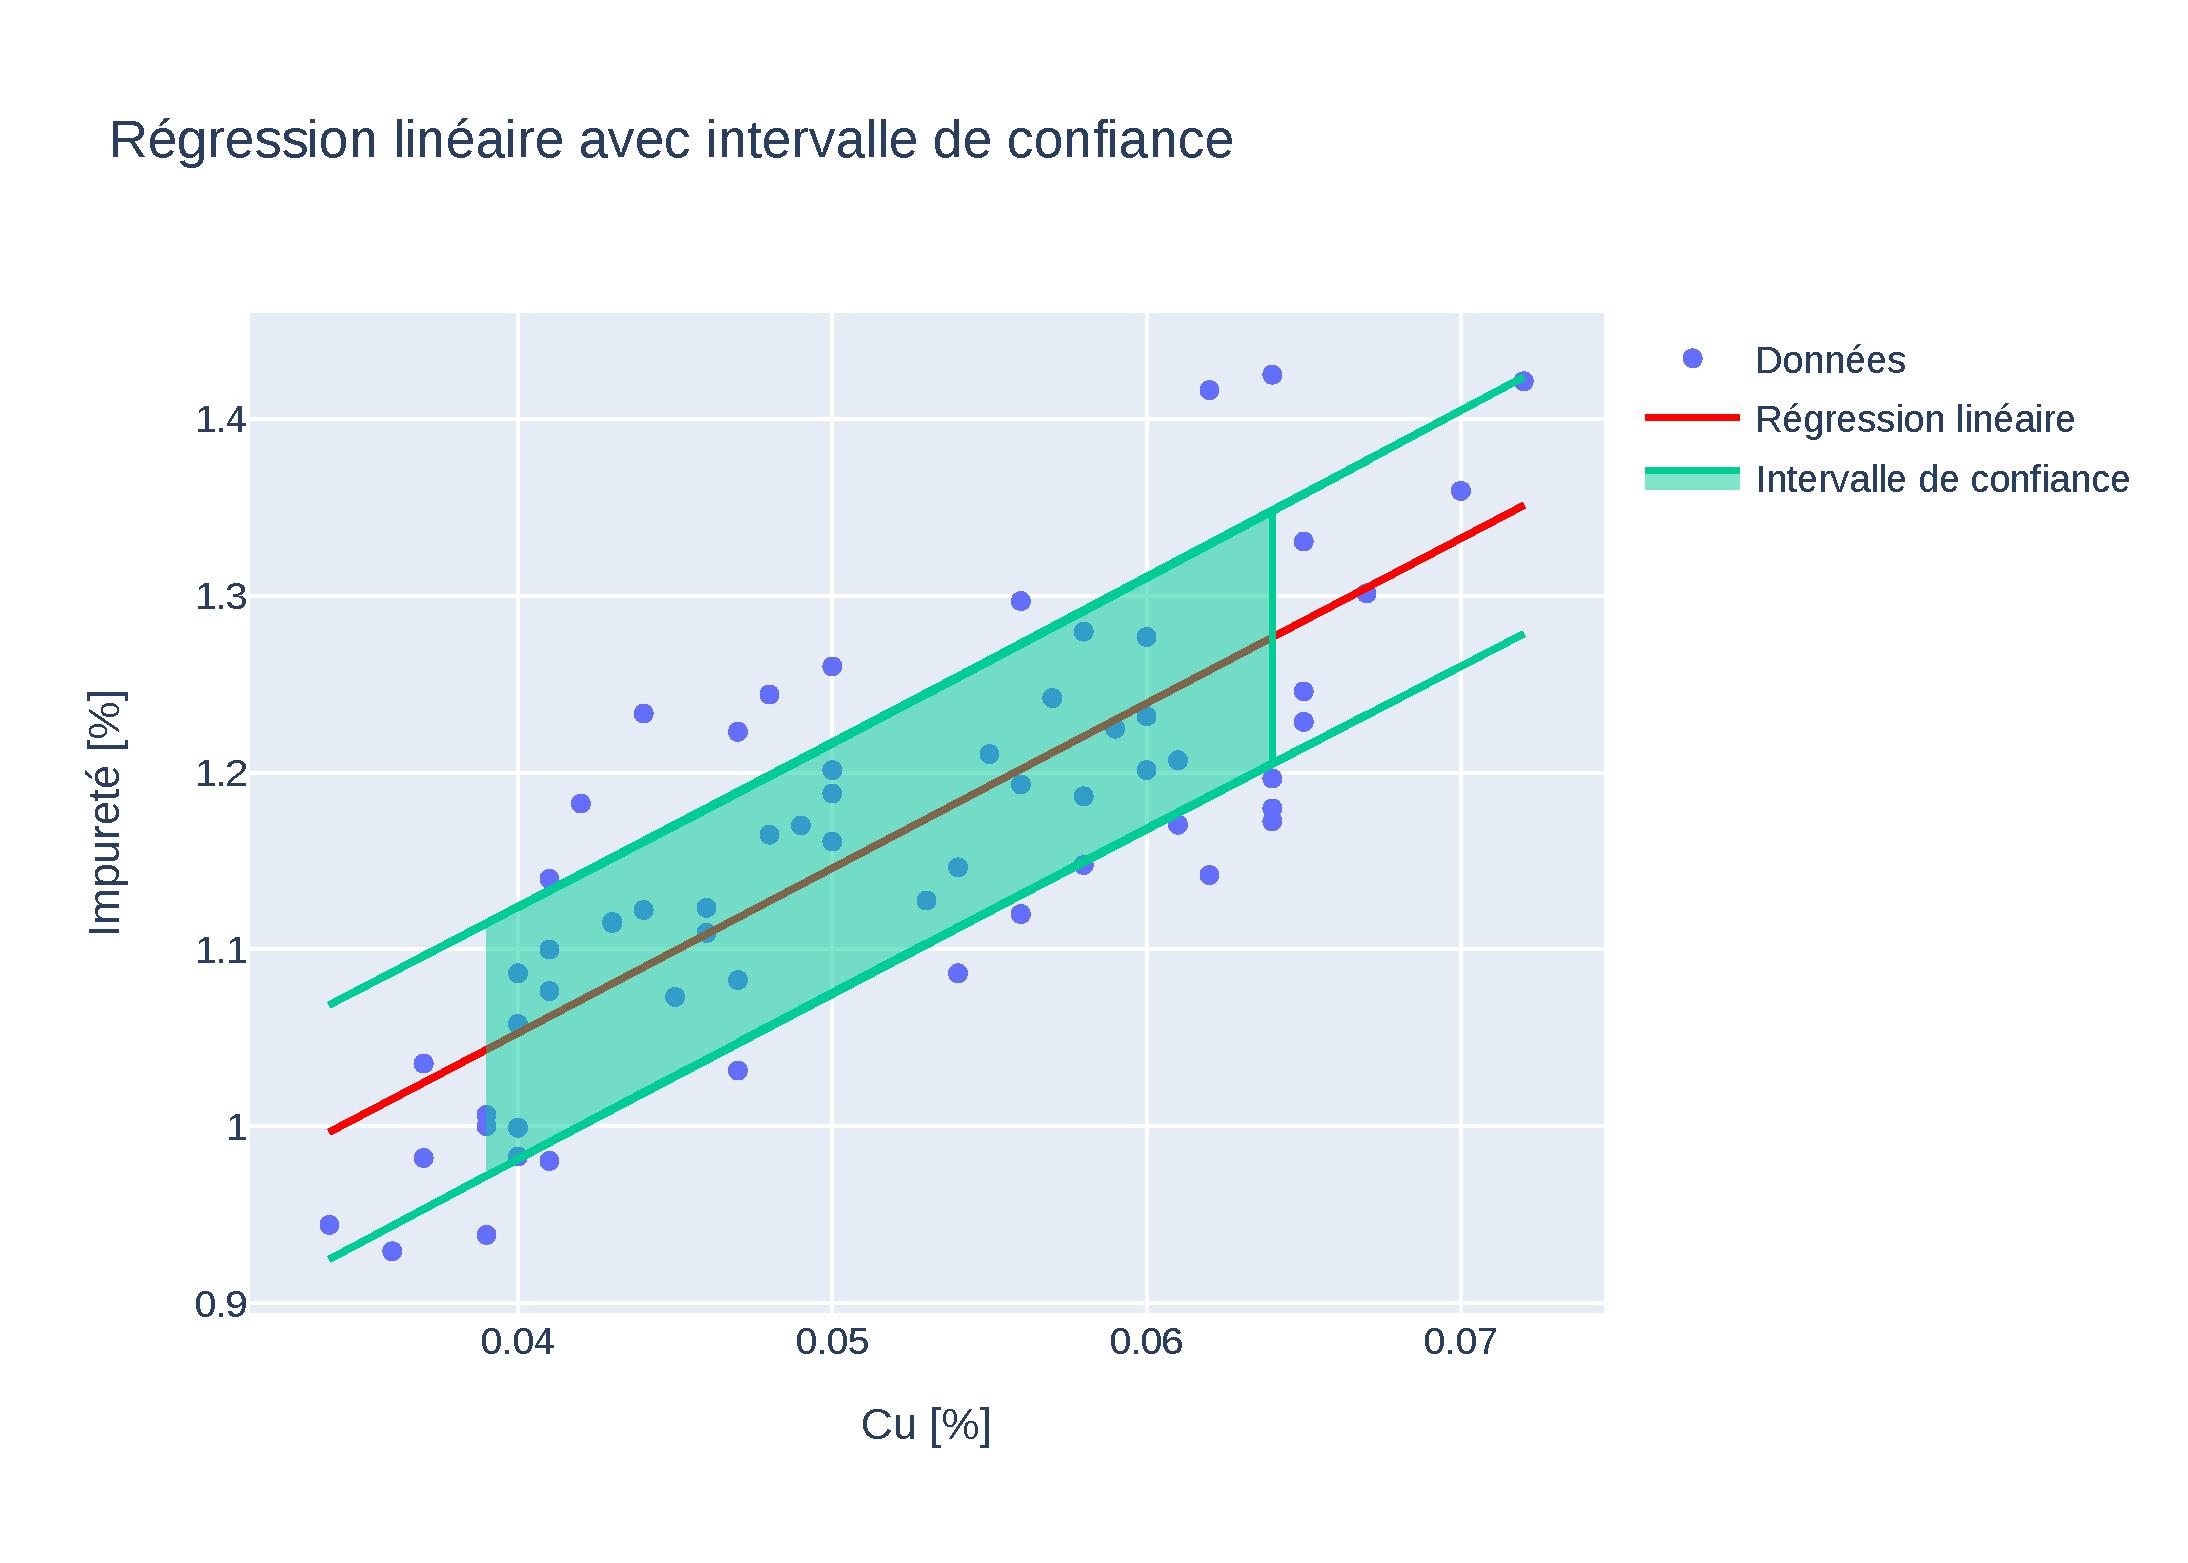
\includegraphics[width=\textwidth]{Images/Statistique/Regression_Impurete_Cu.pdf}
        \end{minipage}
    }\\[0.5cm]  % Espacement vertical entre les rangées
    \adjustbox{width=1.25\textwidth, center}{
        \begin{minipage}{0.8\textwidth}
            \centering
            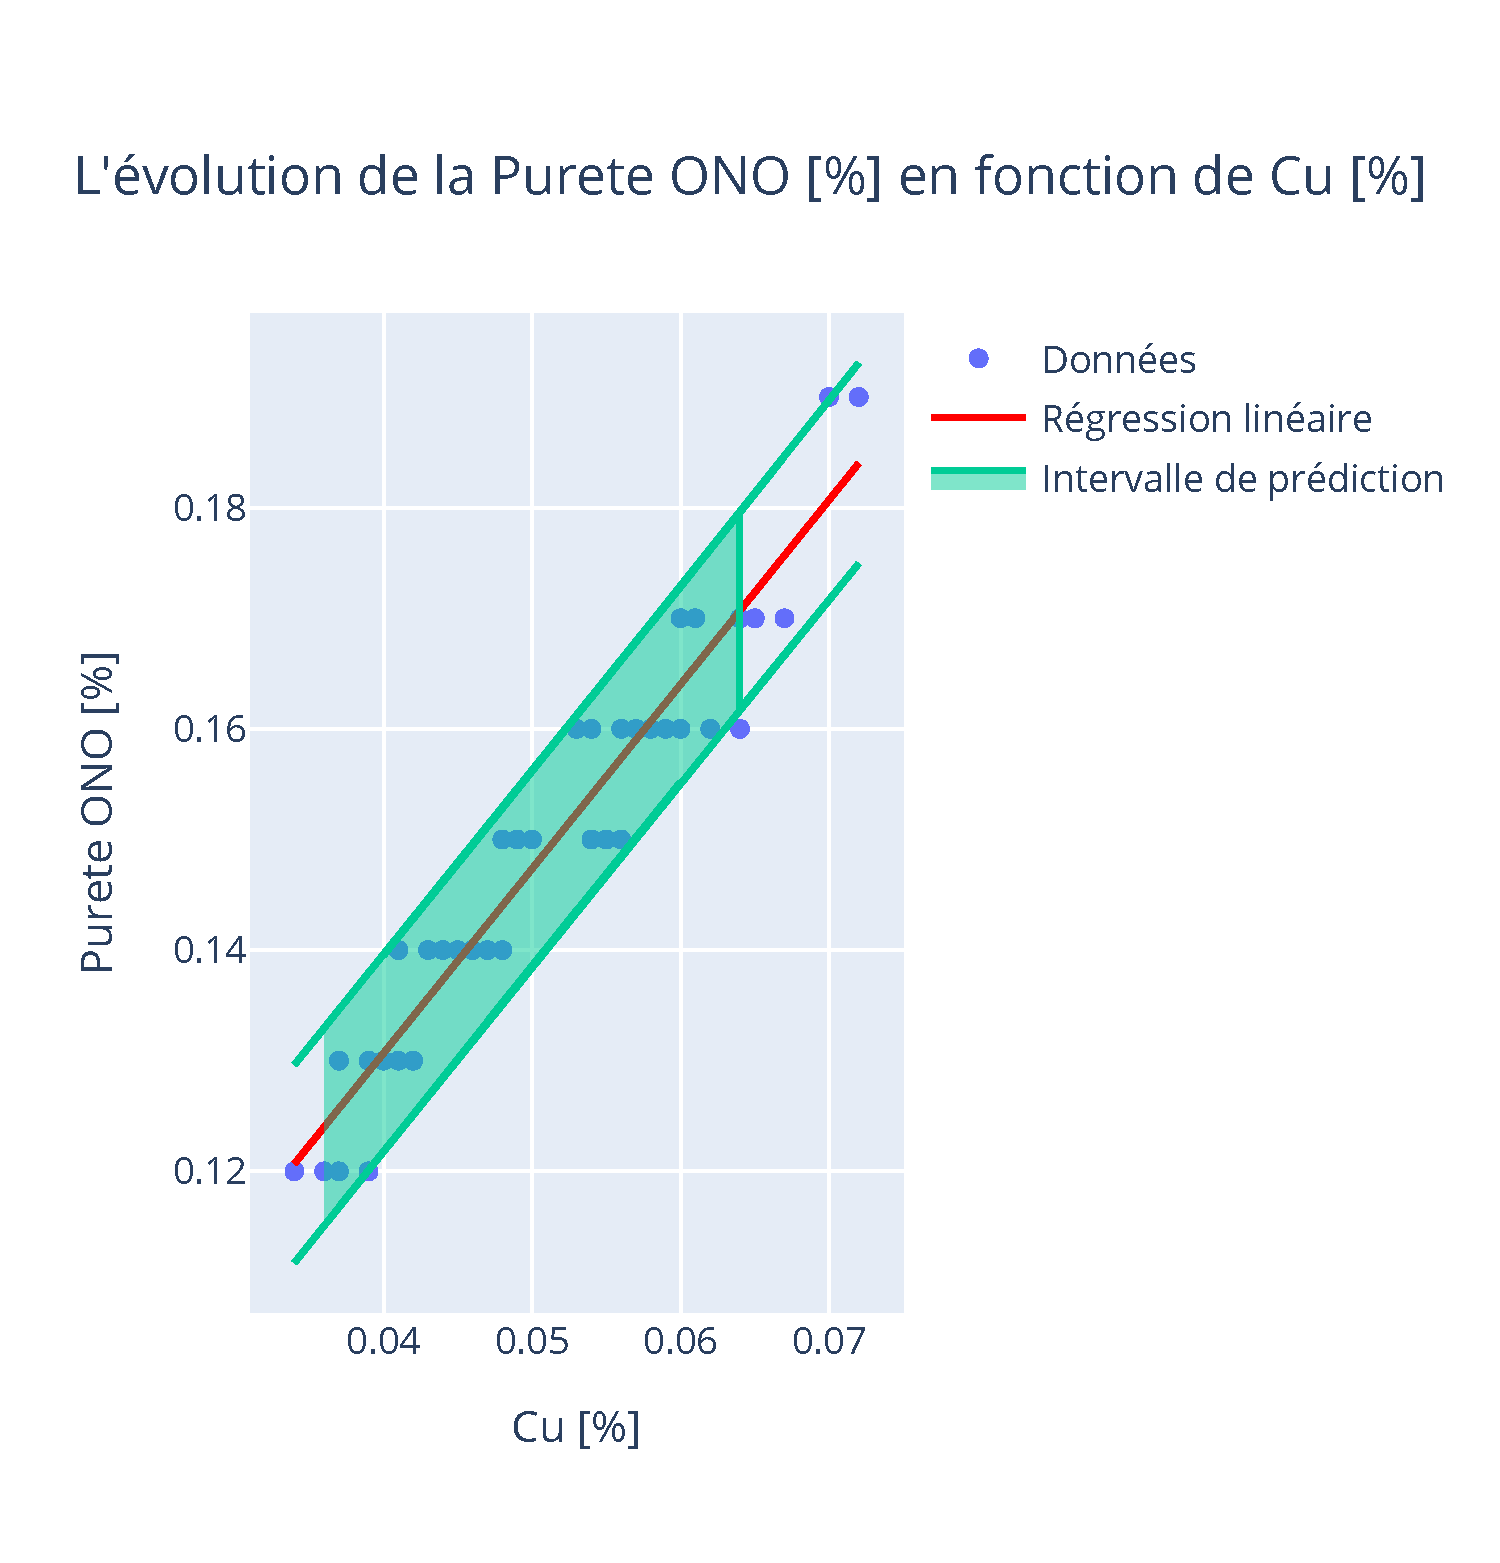
\includegraphics[width=\textwidth]{Images/Statistique/Regression_Ono_Cu.pdf}
        \end{minipage}
        \hspace{0.01\textwidth}  % Petit espacement entre les colonnes
        \begin{minipage}{0.8\textwidth}
            \centering
            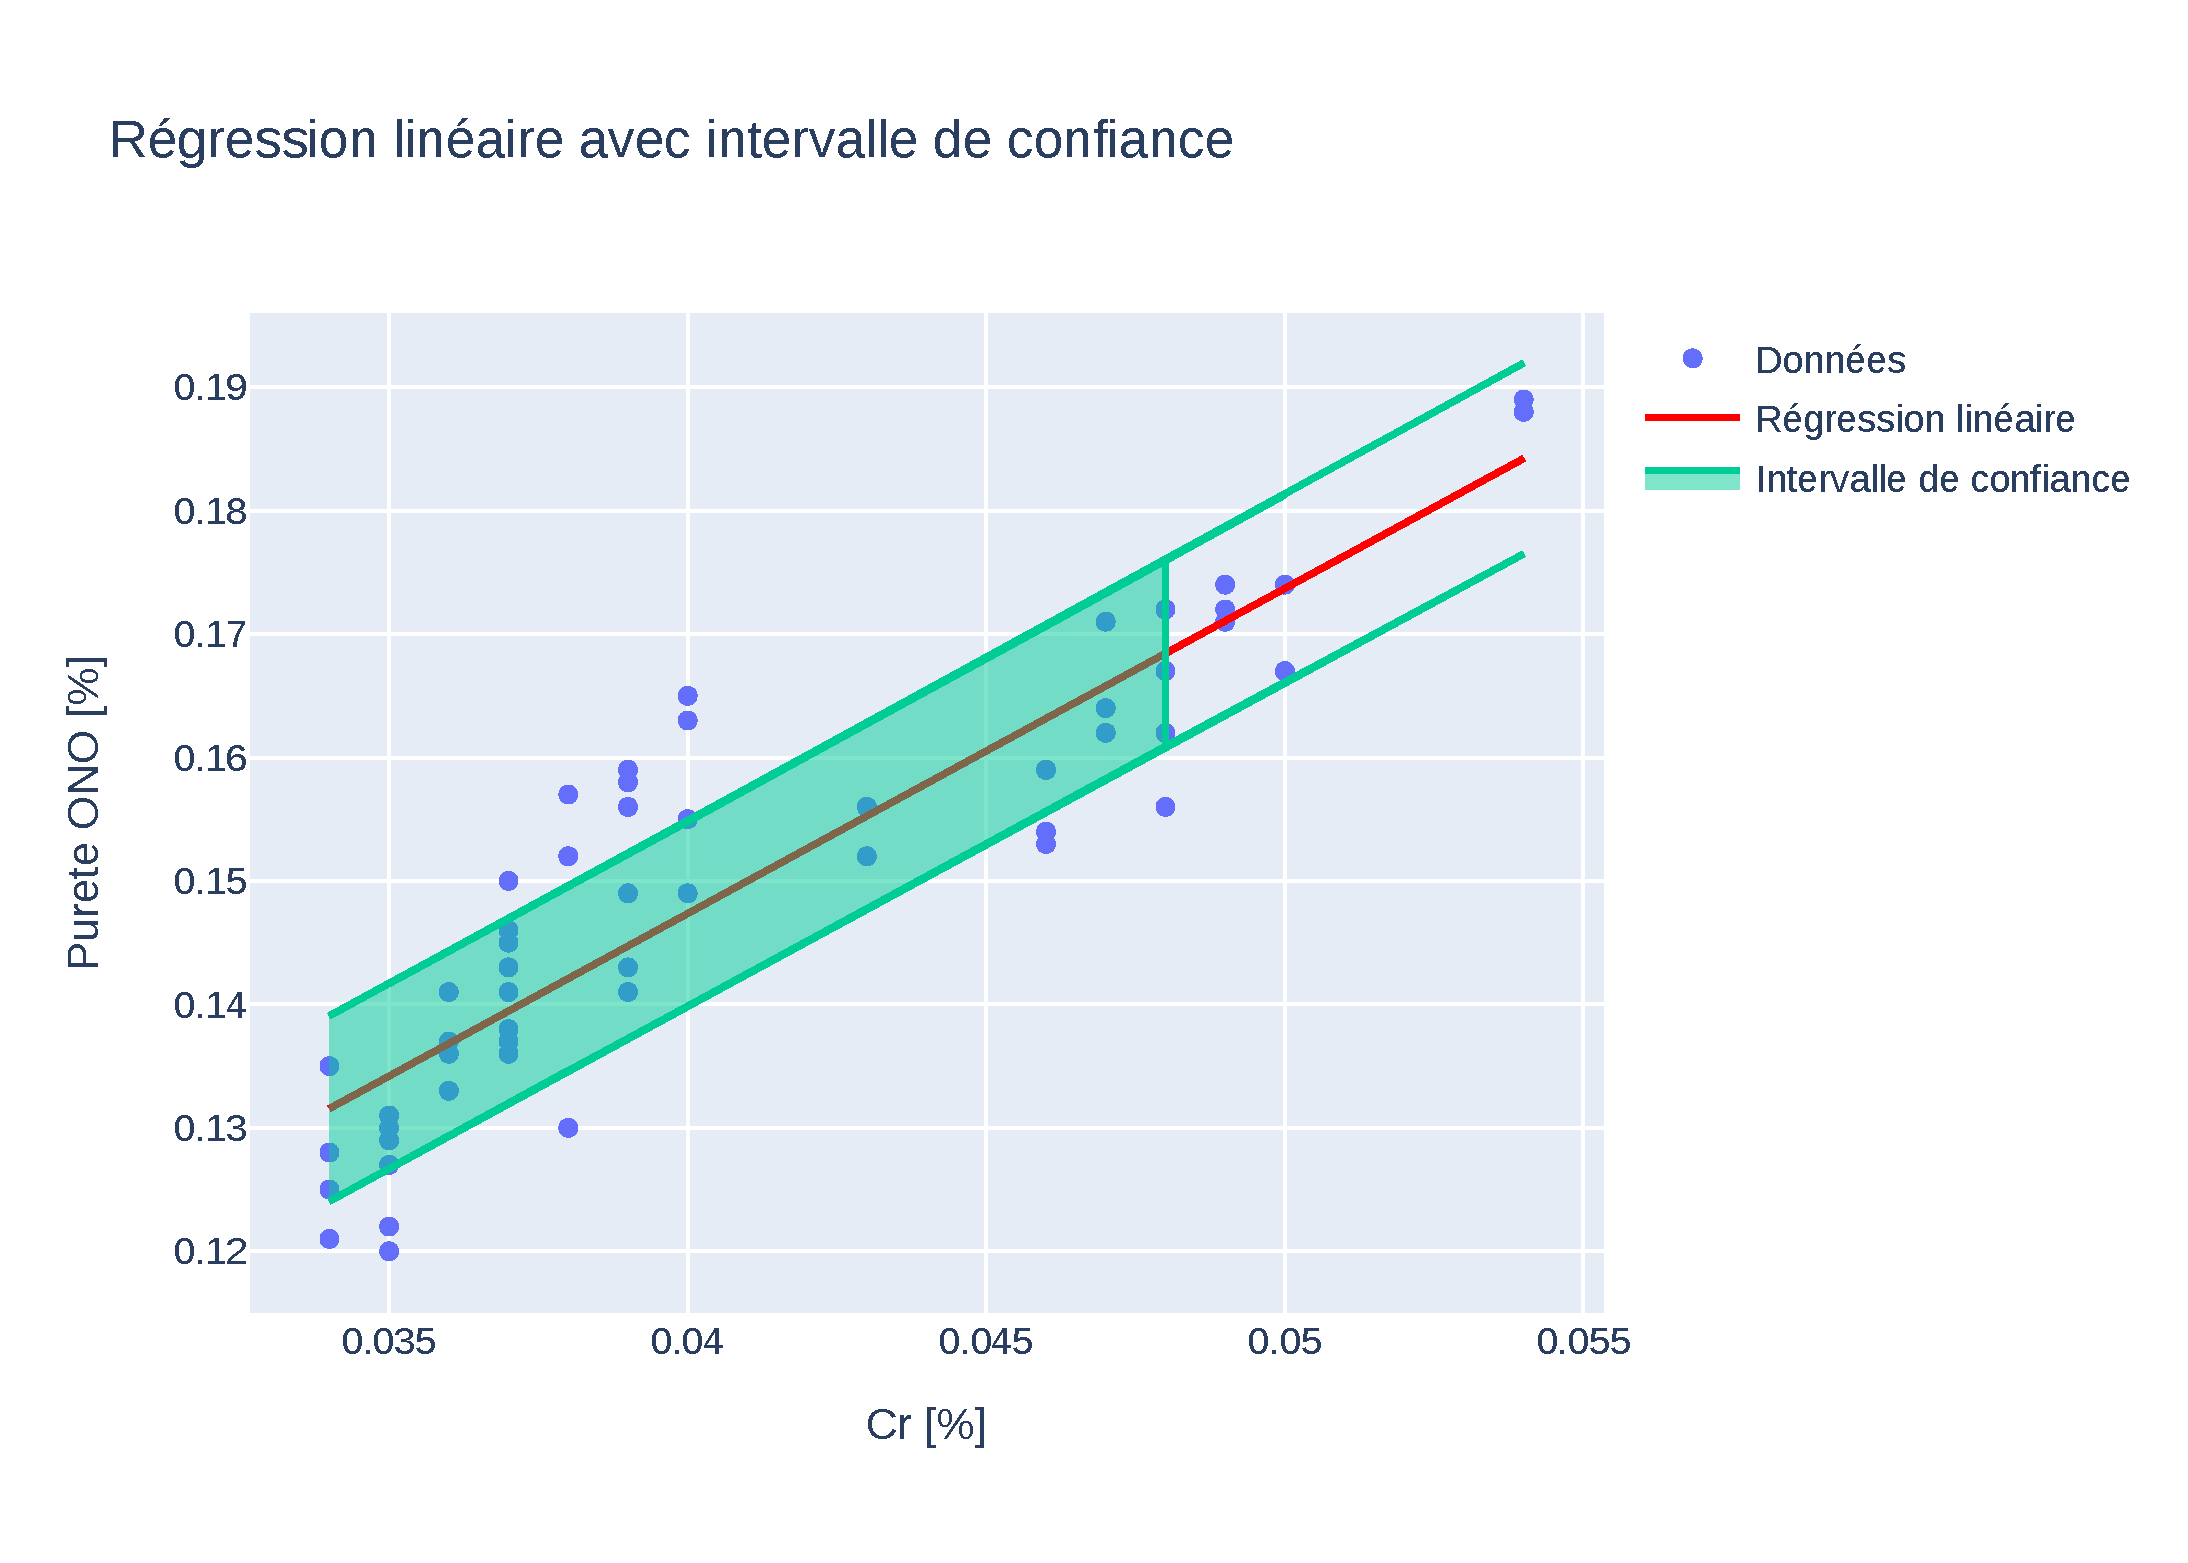
\includegraphics[width=\textwidth]{Images/Statistique/Regression_Ono_Cr.pdf}
        \end{minipage}
    }
    \caption{L'impureté et la pureté Ono en fonction de Sn, de Cr et de Cu}
    \label{fig:regression}
\end{figure}




% Regression linéaire entre Rm et Sn, Cu
% Allongement et Rm
\begin{figure}[H]
    \centering
    \adjustbox{width=1.25\textwidth, center}{  % Ajuste la largeur à la page
        \begin{minipage}{0.8\textwidth}
            \centering
            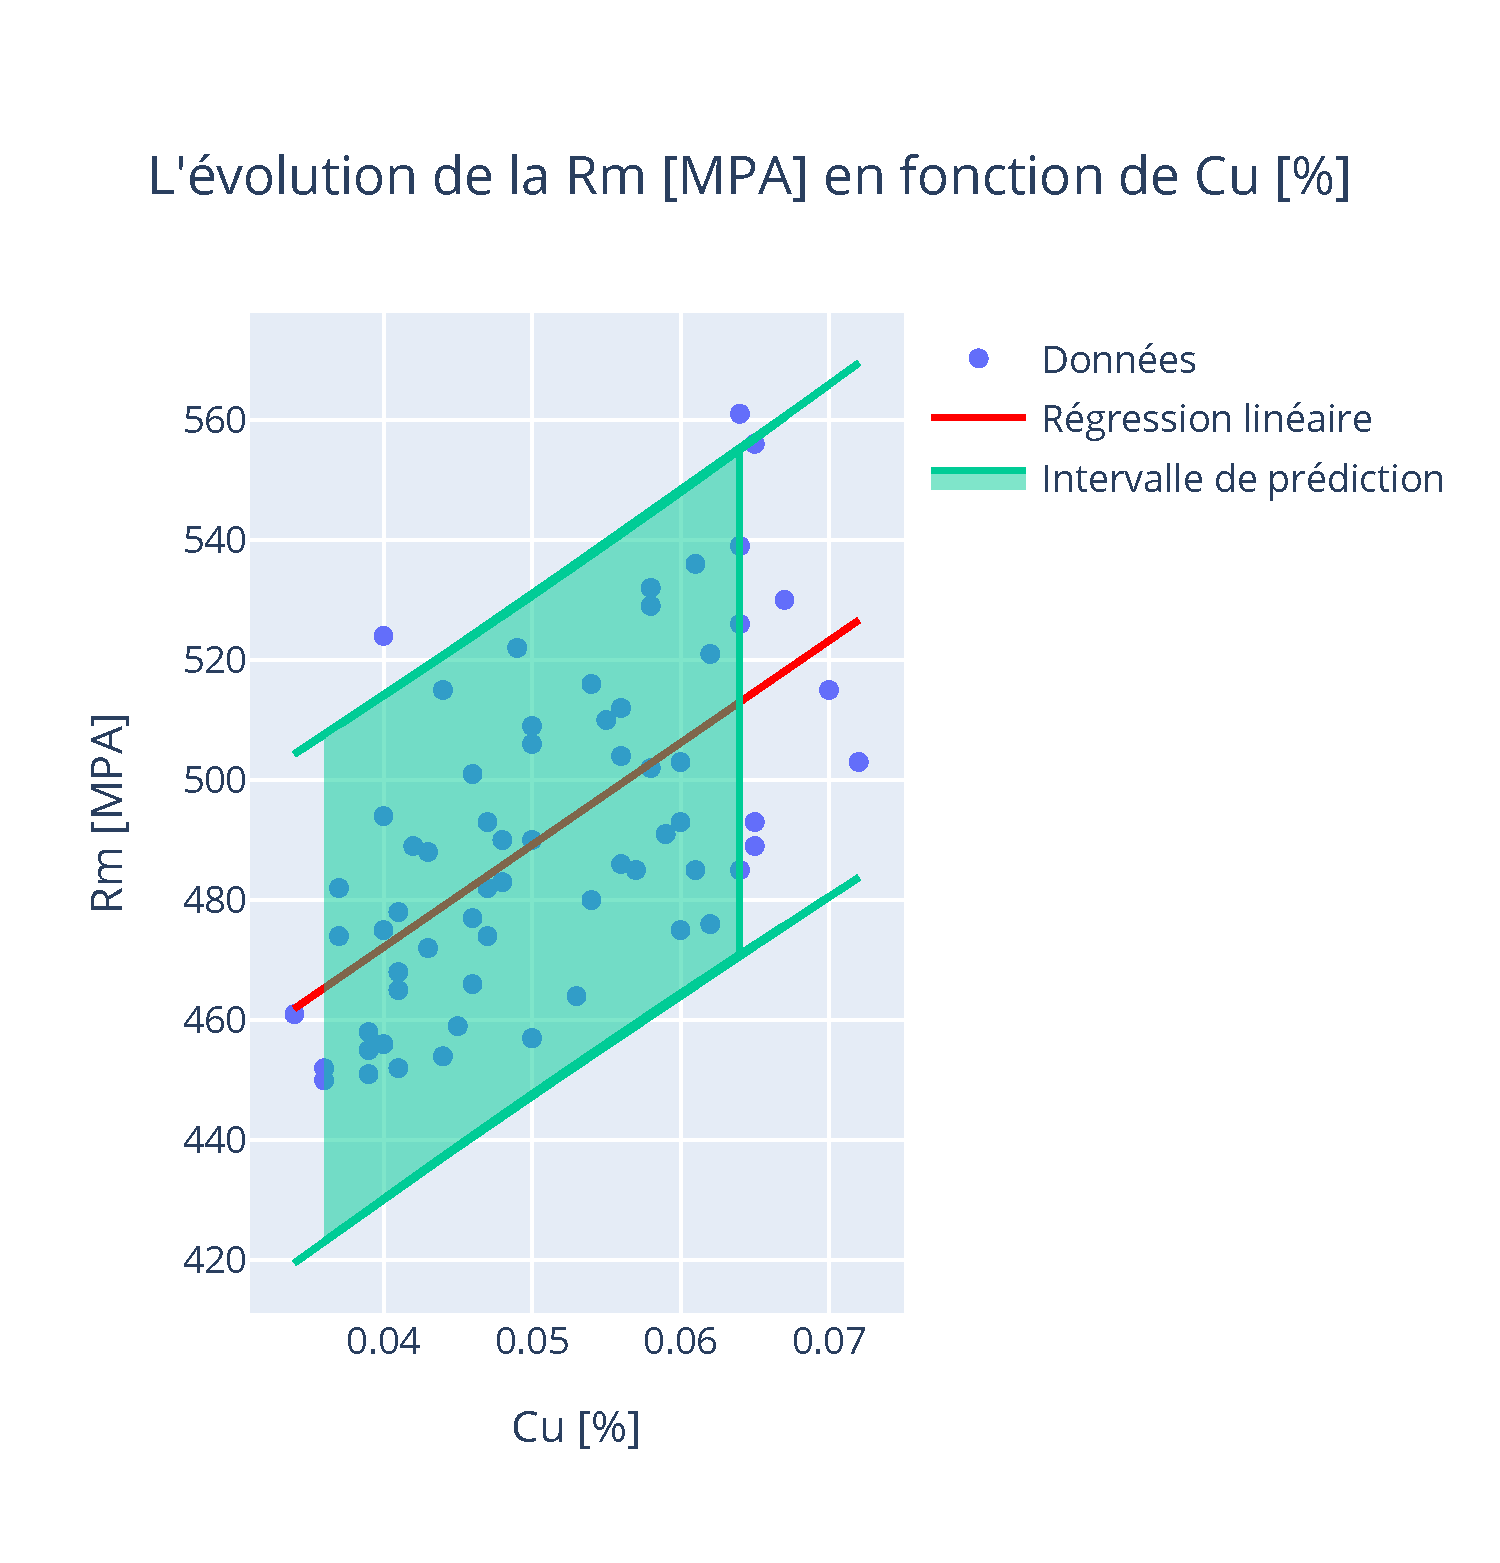
\includegraphics[width=\textwidth]{Images/Statistique/Regression_Cu_Rm.pdf}
        \end{minipage}
        \hspace{0.01\textwidth}  % Petit espacement entre les colonnes
        \begin{minipage}{0.8\textwidth}
            \centering
            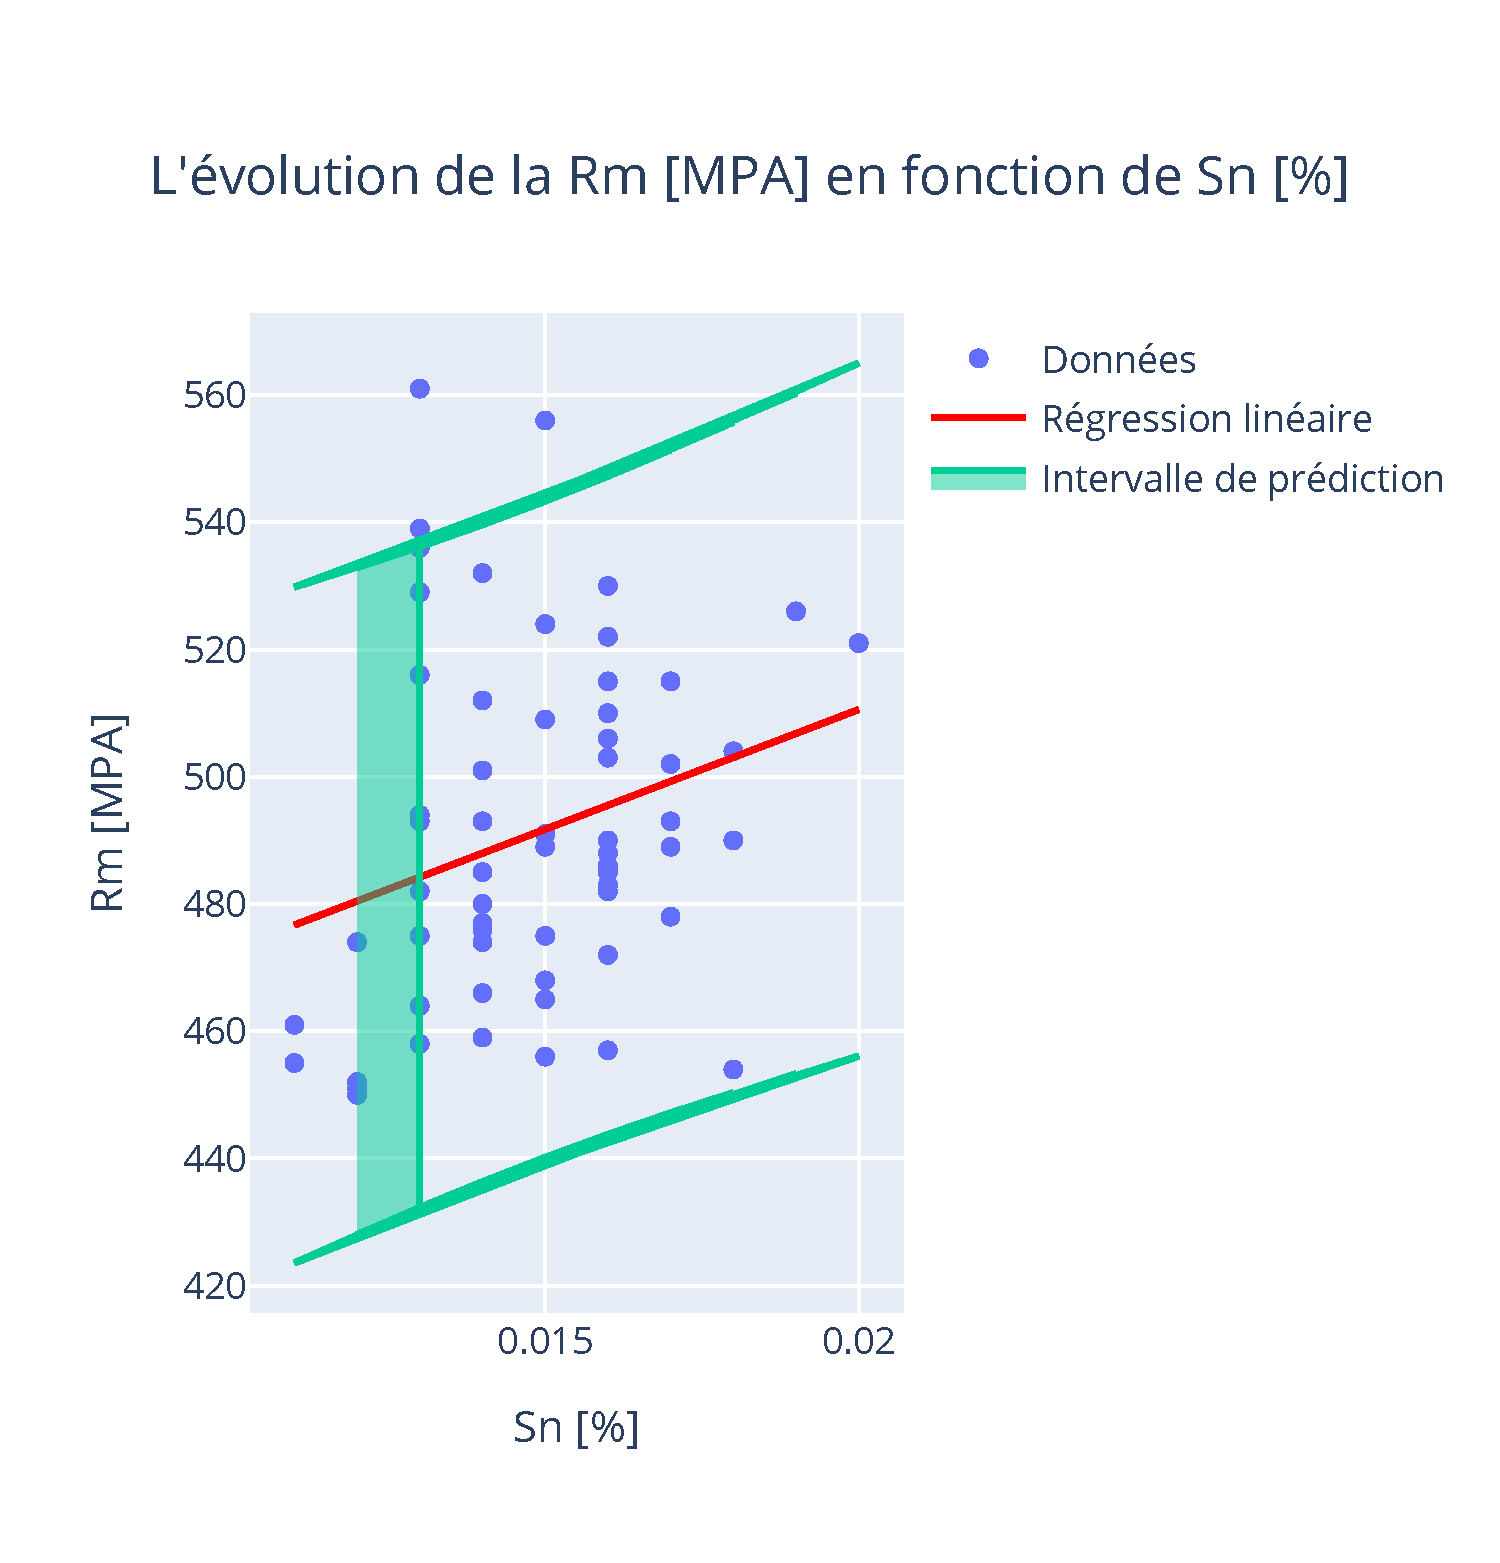
\includegraphics[width=\textwidth]{Images/Statistique/Regression_Sn_Rm.pdf}
        \end{minipage}
    }\\[0.5cm]  % Espacement vertical entre les rangées
    \adjustbox{width=1.25\textwidth, center}{
        \begin{minipage}{0.8\textwidth}
            \centering
            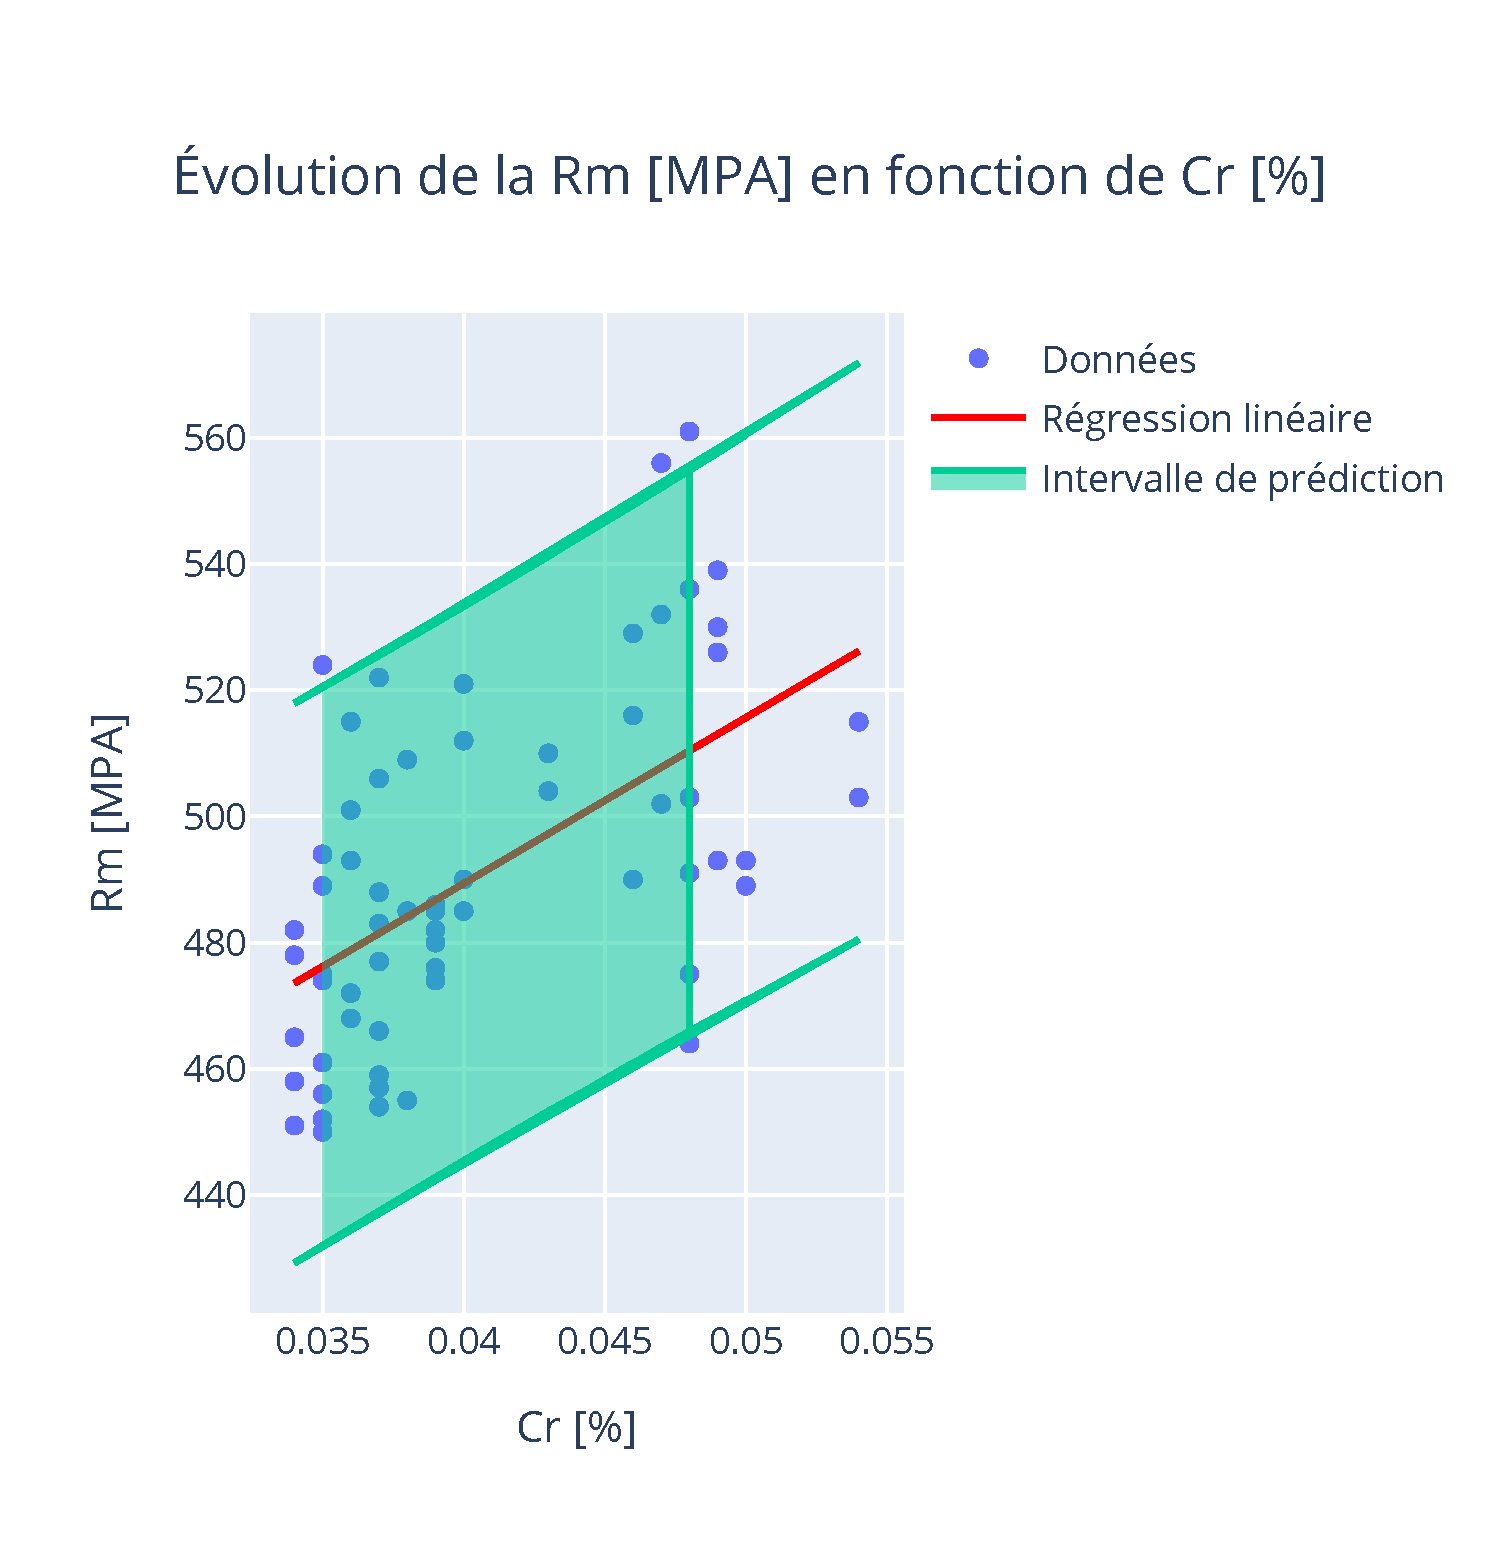
\includegraphics[width=\textwidth]{Images/Statistique/Regression_Cr_Rm.pdf}
        \end{minipage}
        \hspace{0.01\textwidth}  % Petit espacement entre les colonnes
        \begin{minipage}{0.8\textwidth}
            \centering
            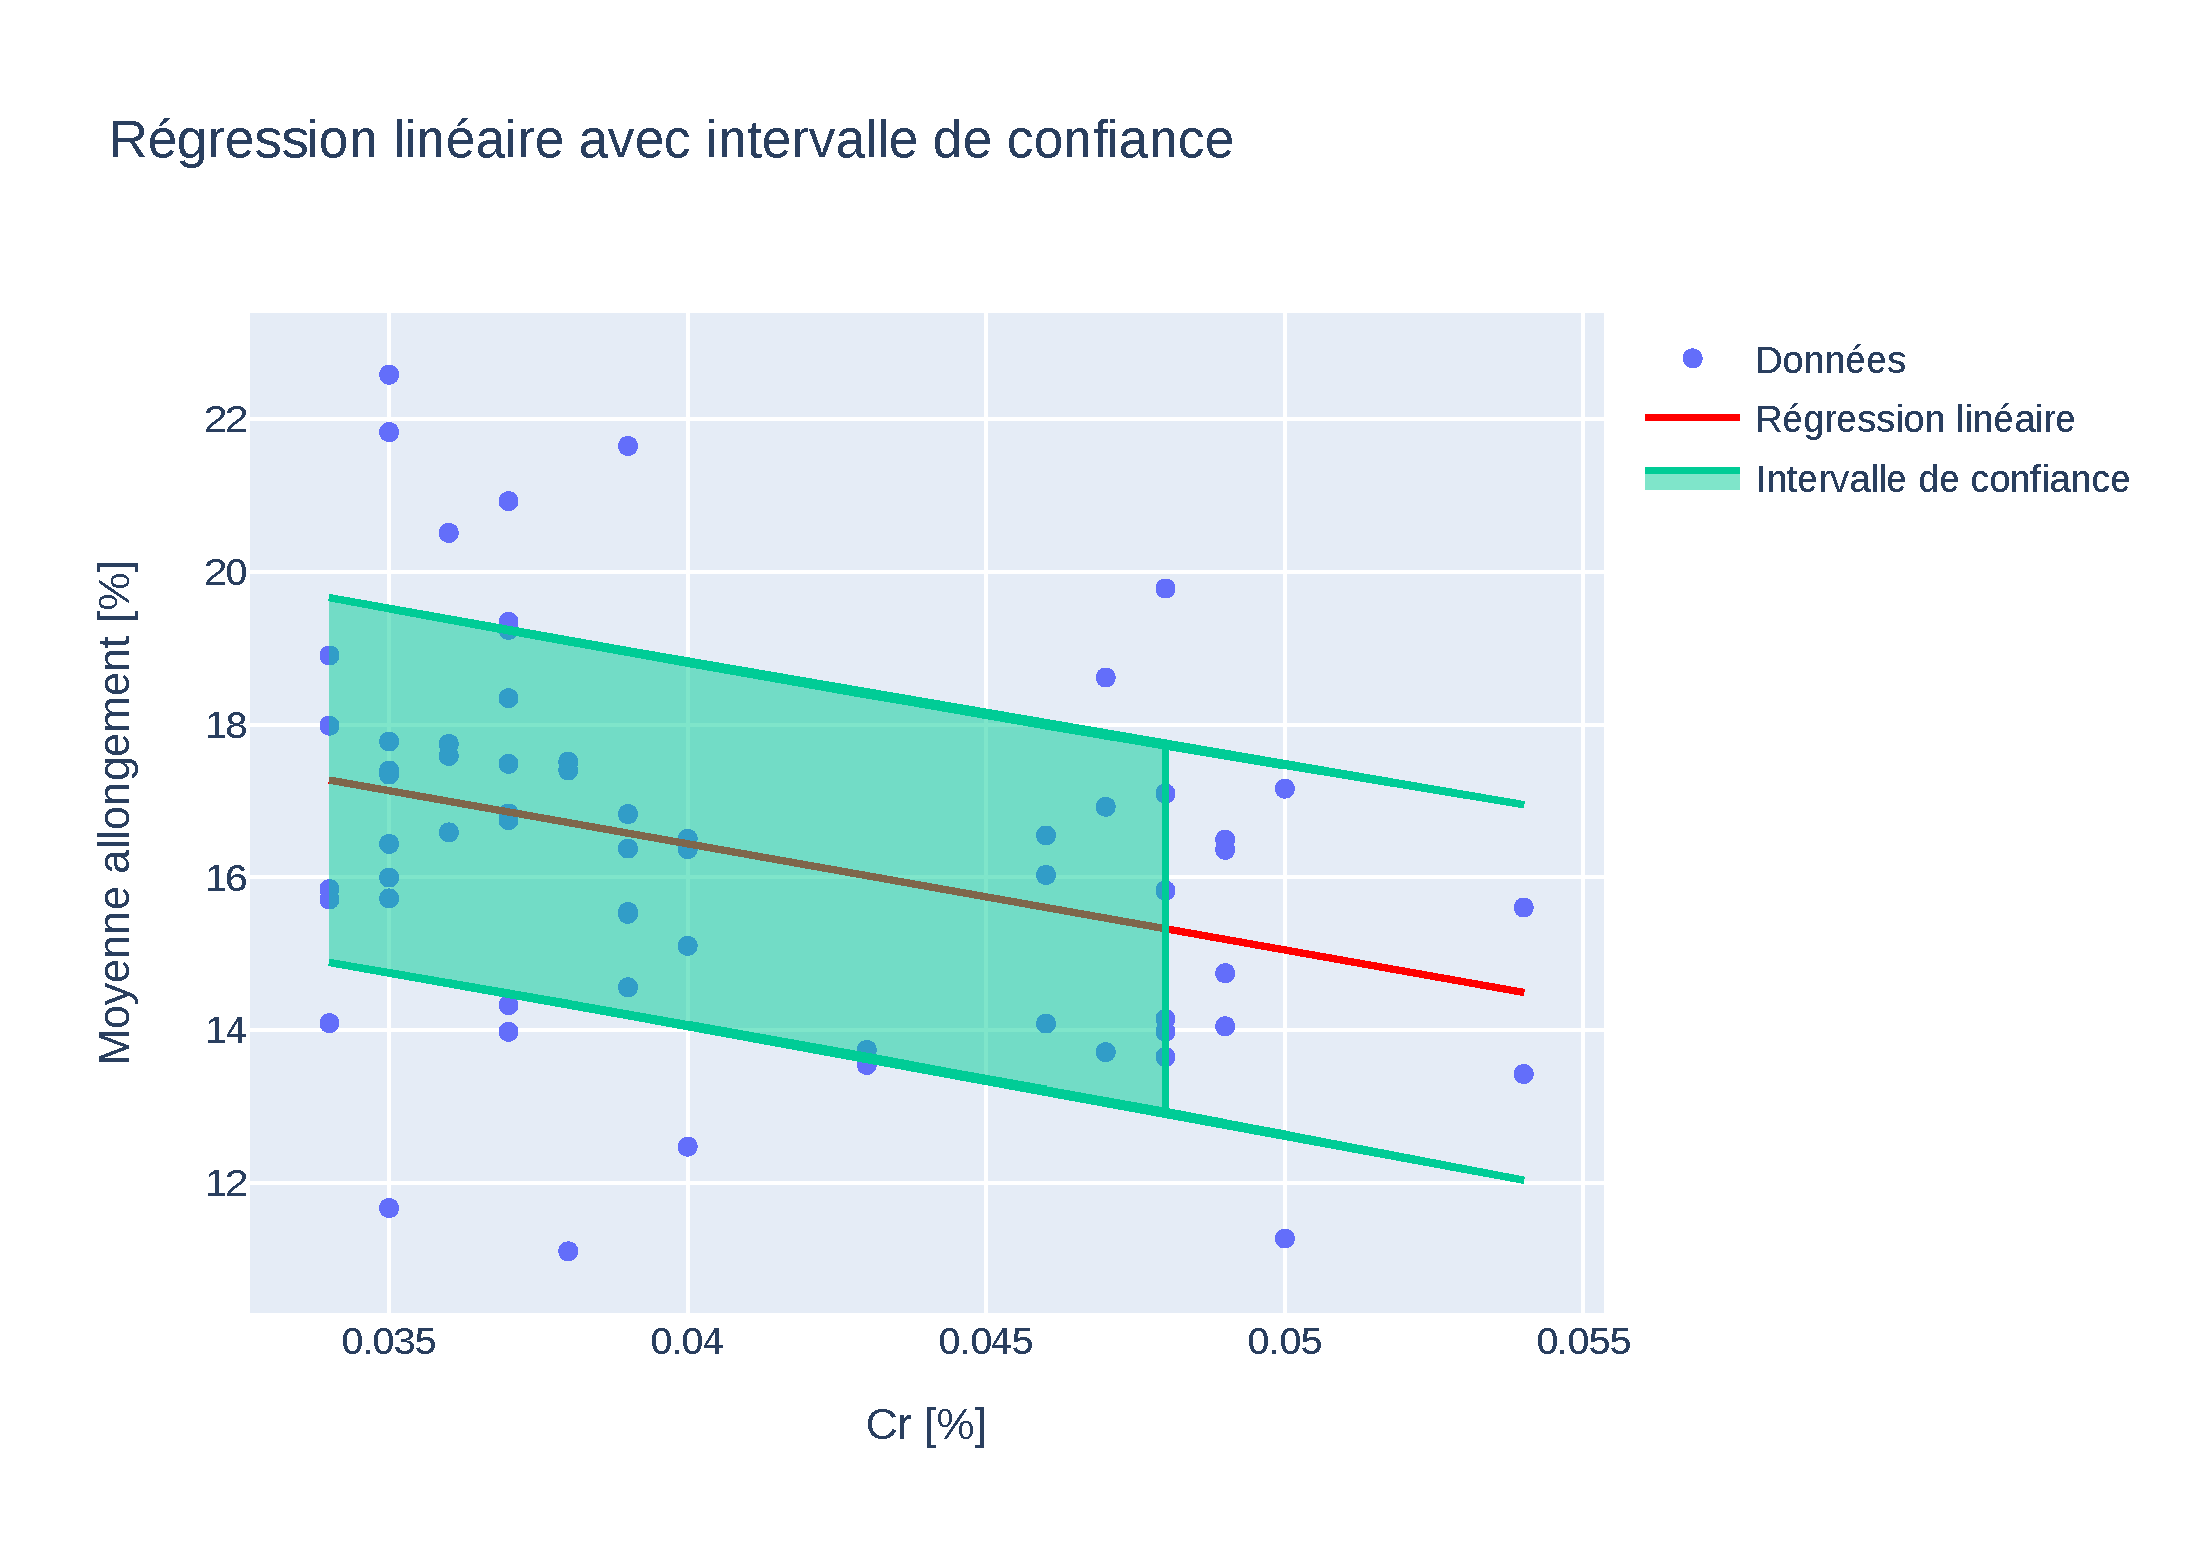
\includegraphics[width=\textwidth]{Images/Statistique/Regression_Cr_Allongement.pdf}
        \end{minipage}
    }
    \caption{L'allongement et la résistance mécanique en fonction du Cuivre, de Sn, et du Cr}
    \label{fig:regression2}
\end{figure}






% Regression linéaire entre Allongement et Sn, Cu
\begin{figure}[H]
    \centering
    \begin{adjustbox}{width=1.35\textwidth,center}
        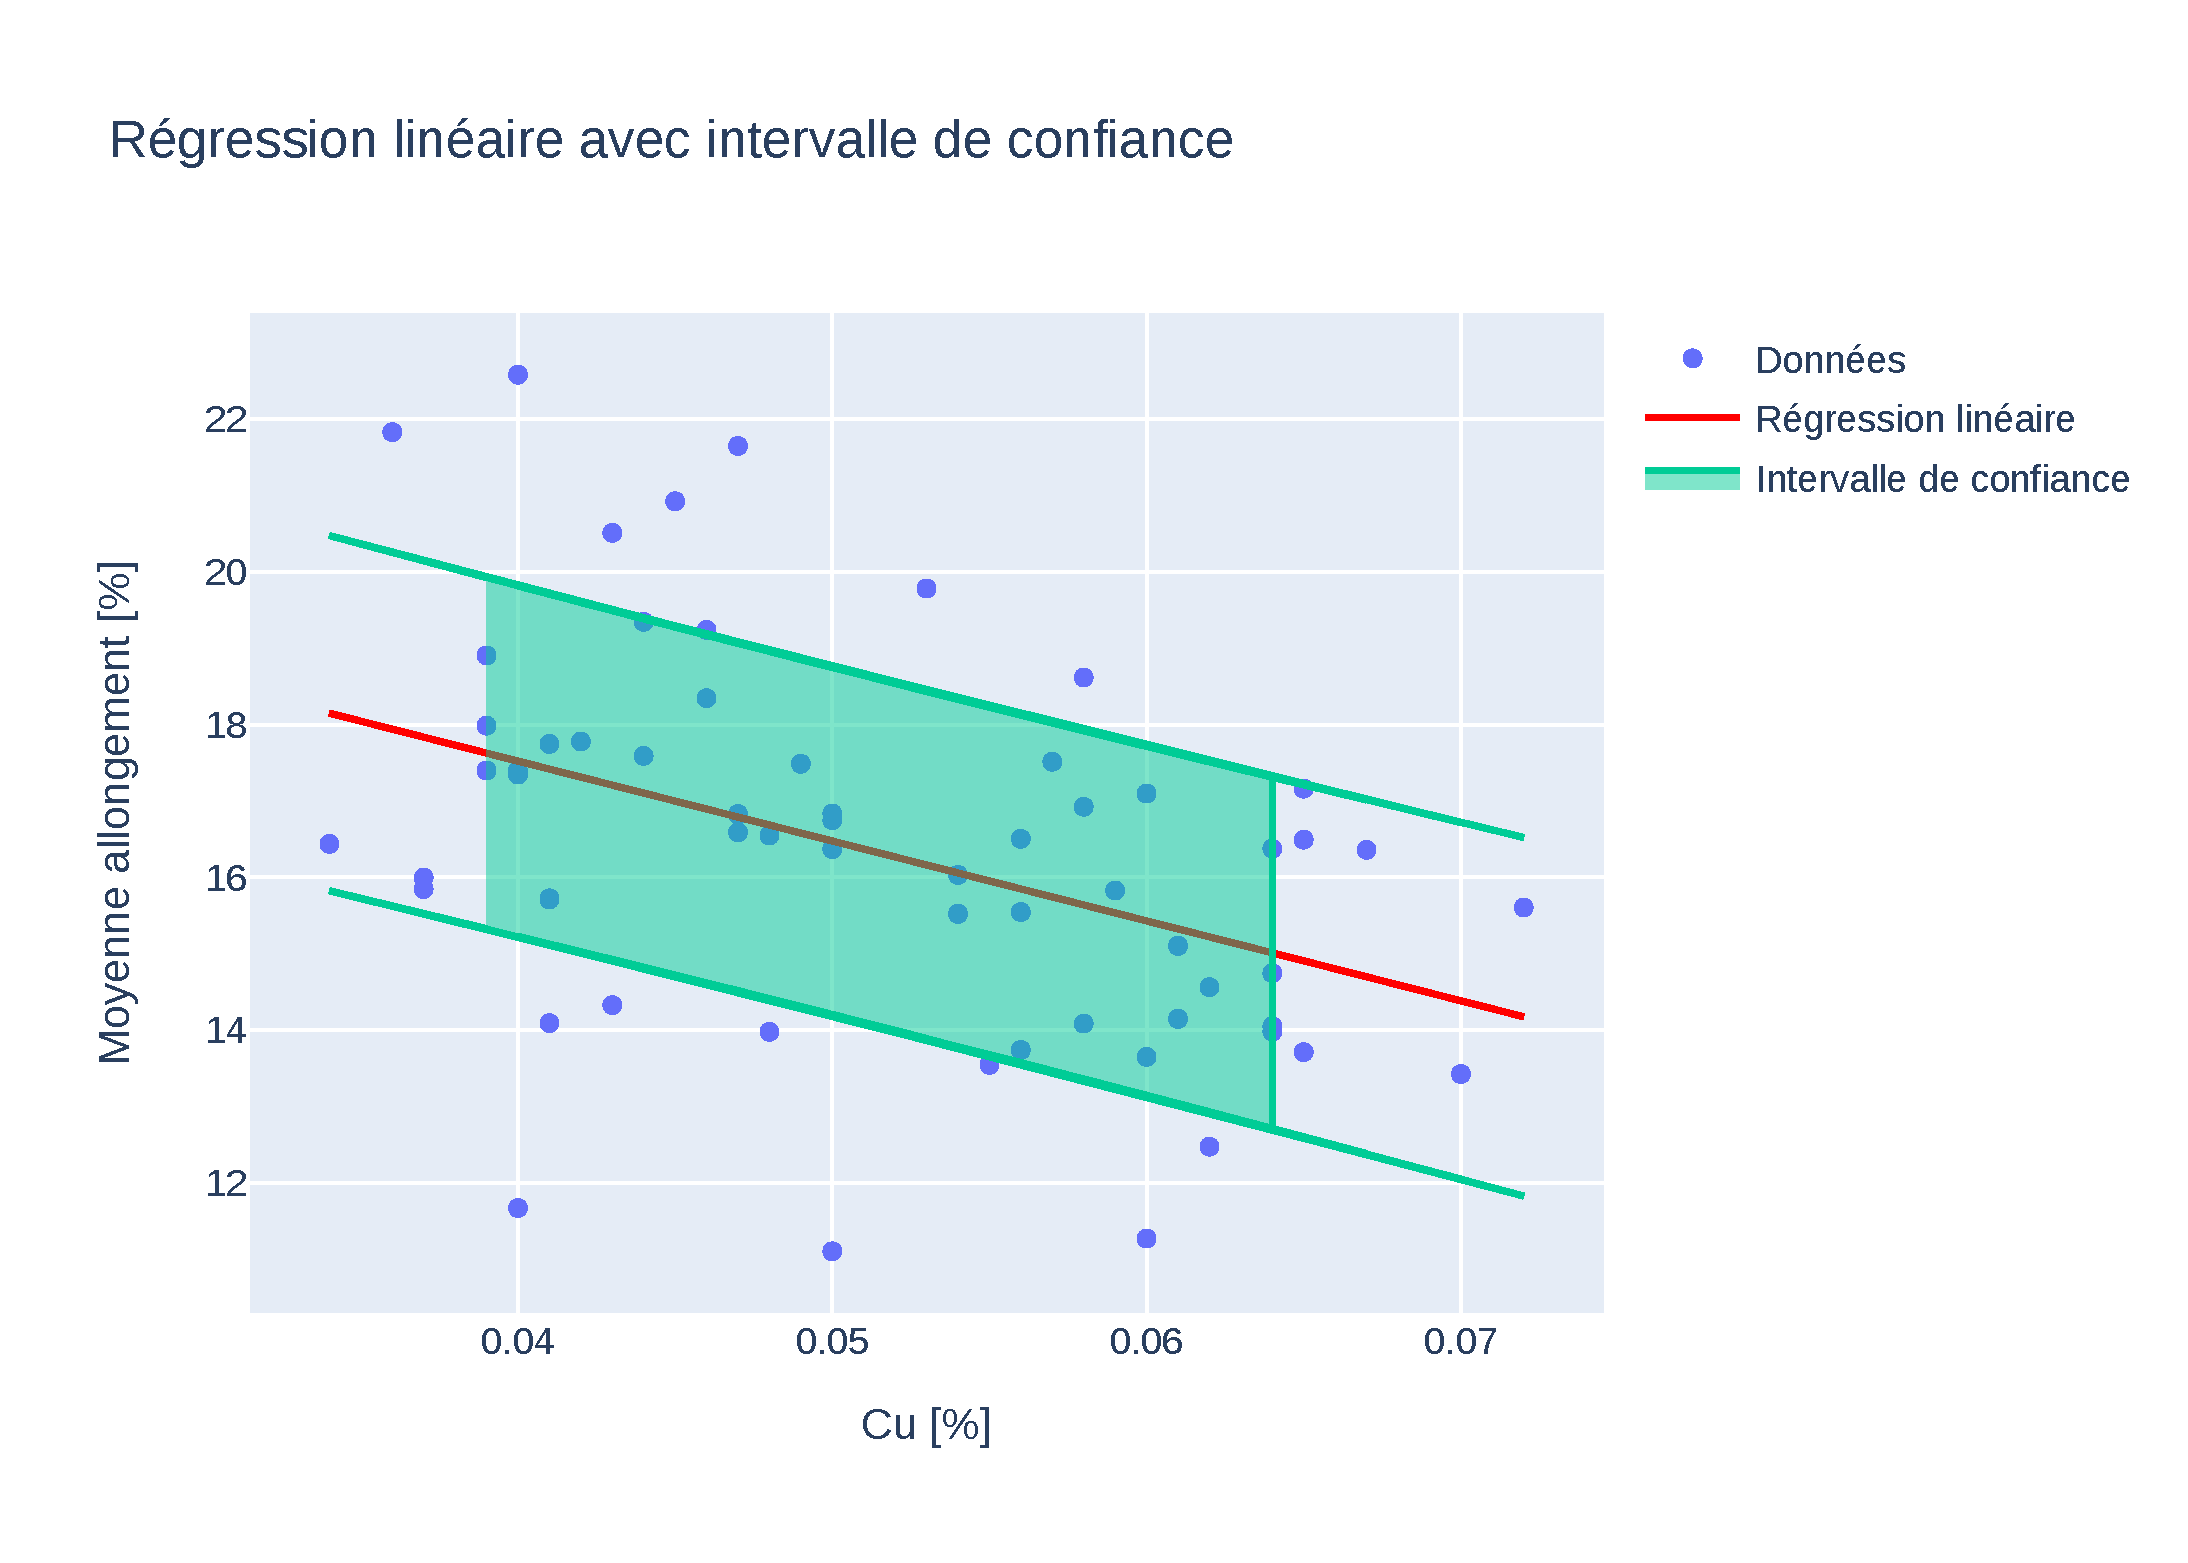
\includegraphics[scale=1]{Images/Statistique/Regression_Cu_Allongement.pdf}
        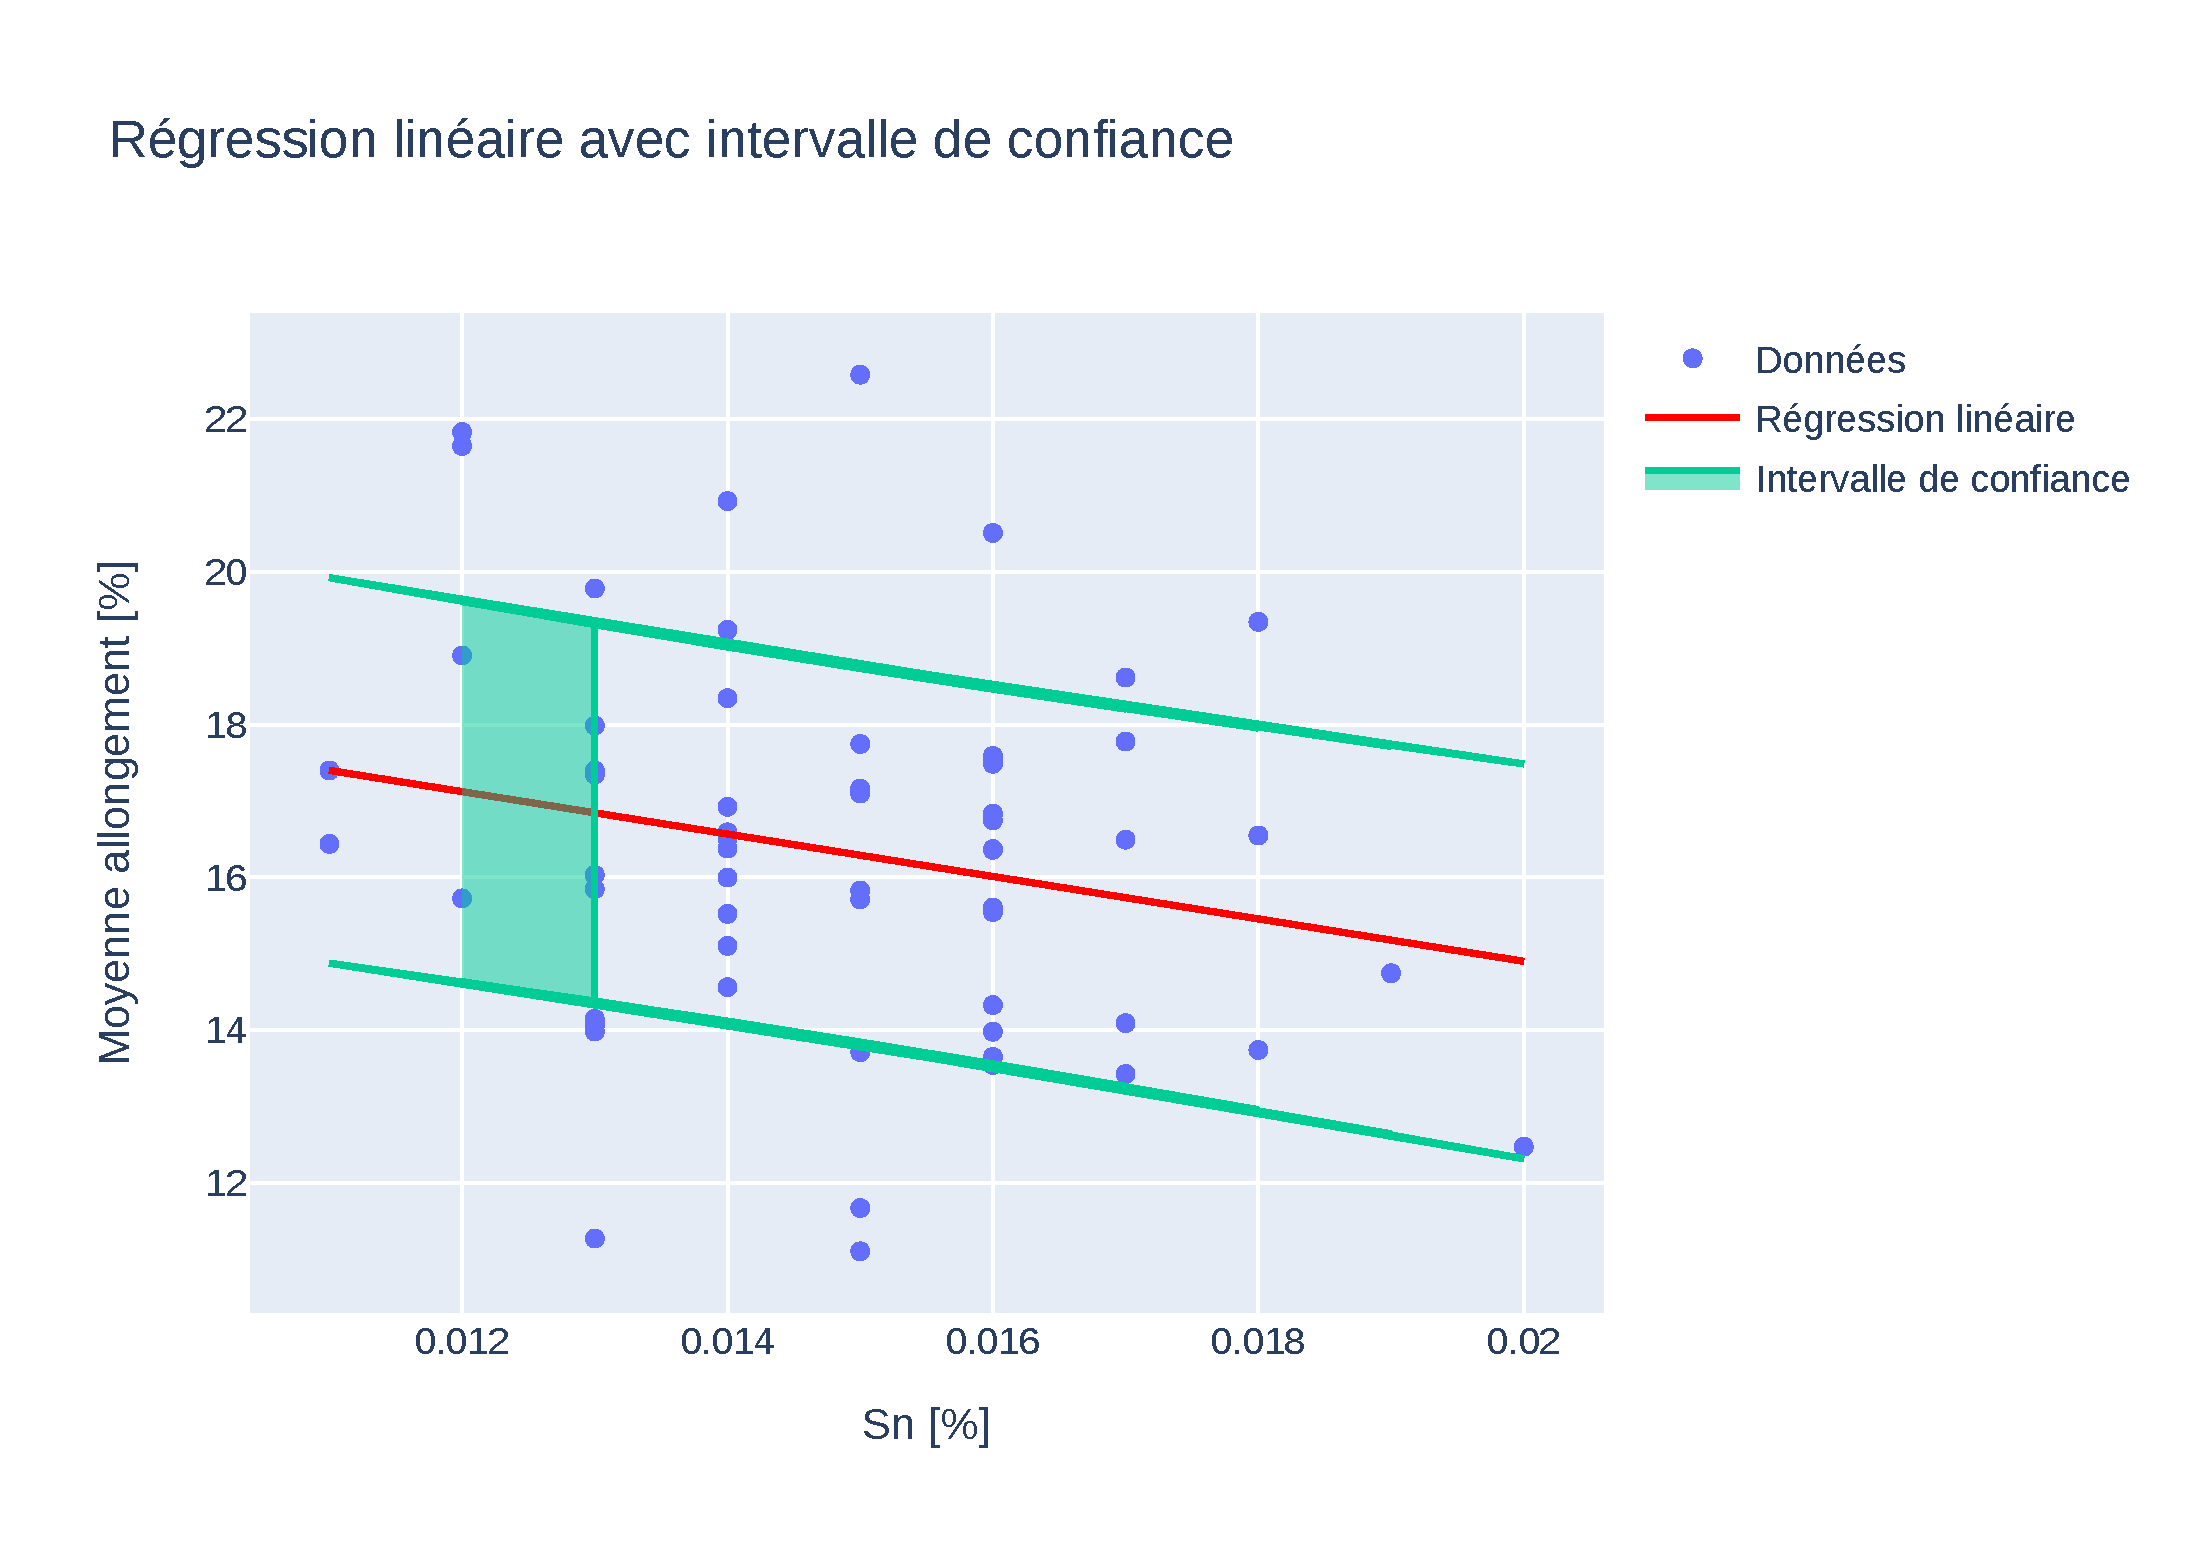
\includegraphics[scale=1]{Images/Statistique/Regression_Sn_Allongement.pdf}
    \end{adjustbox}
    \caption{L'allongement en fonction du Cuivre et  de Sn }
    \label{fig:regression3}
\end{figure}



L'analyse révèle une corrélation linéaire notable entre le cuivre et la 
résistance mécanique, ainsi qu'entre le cuivre et l'allongement, et enfin 
entre la pureté ONO et le cuivre. En revanche, pour les autres éléments 
chimiques, la relation linéaire n'est pas évidente, même en élargissant 
les intervalles de prédiction. Dans ces cas, il est donc plus pertinent 
de se baser sur les intervalles de confiance.

\textbf{Intervalles de confiance des indicateurs :}
\begin{itemize}
\item Impureté : [1.13, 1.19]
\item Pureté ONO : [0.145, 0.153]
\end{itemize}

\textbf{Intervalles de confiance des éléments chimiques :}
\begin{itemize}
\item Sn (Étain) : [0.0143, 0.0153]
\item Cu (Cuivre) : [0.0488, 0.0538]
\item Cr (Chrome) : [0.0392, 0.0422]
\item V (Vanadium) : [0.00092, 0.00111]
\end{itemize}





\subsection*{Conclusion}

Compte tenu de la quantité limitée de données disponibles, l'analyse 
statistique réalisée sur les données de la fonte GS 450-10 ne s'avère 
pas concluante. L'impureté et la pureté ONO ont été sélectionnées comme 
les meilleurs substituts à la résistance mécanique et à l'allongement, 
en se basant sur les matrices de corrélation. Cependant, lorsqu'il s'agit 
de déterminer les valeurs optimales de ces indicateurs afin de garantir 
la conformité de la fonte, les résultats obtenus ne sont pas significatifs.





\section{La recette Optimale}

\subsection{Présentation du problème}

Dans le cadre du processus de fabrication de 5 tonnes de fontes, l'une des
étapes préliminaires fondamentales réside dans la détermination du lit de
fusion, c'est-à-dire la proportion des matières premières nécessaires à la 
fusion. Dans notre cas, on souhaite produire 5 tonnes de fonte de haute 
qualité.

Pour ce faire, nous disposons d'une trentaine de matières premières, 
chacune possédant sa propre composition chimique distinctive. Chaque 
matière première est disponible ou non en quantité limitée et leurs prix 
varient tout au long de l'année. Ces matières sont issues de diverses 
sources, comprenant des matériaux métalliques et de construction, ainsi 
que des retours, c'est-à-dire des résidus provenant des précédents cycles 
de production.

Par exemple, parmi ces matériaux, on trouve les sabots de freins SNCF, les 
rails de chemin de fer de 40 cm et de la fonte GS recyclée, dont les prix 
respectifs sont de 435 euros, 423,90 euros et 374 euros par tonne.

La qualité de la fonte dépend de sa composition chimique, qui doit se 
situer dans des intervalles spécifiques adaptés au type de fonte recherché,
tout en respectant des critères de qualité tels que le niveau d'impuretés 
et la pureté ONO. Le niveau d'impuretés et la pureté ONO sont déterminés 
par des combinaisons linéaires des pourcentages d'éléments chimiques 
présents dans les matières premières.

Par conséquent, l'objectif principal est de déterminer les proportions 
optimales des matières premières, en vue de minimiser les coûts de 
production tout en préservant la qualité de la fonte.


% Modélisation du problème ou Formulation mathématique du problème




\subsection{ Modélisation du problème }

Pour modéliser ce problème de manière optimale, nous avons proposé 
deux formulation du problème. La première formulation consiste à résoudre 
le problème suivant :

\[
\underset{\mathbf{x}}{\min} \, \mathbf{C} \cdot \mathbf{x}
\]

sous les contraintes :

$$
\begin{cases}
\mathbf{A}_{eq} \cdot \mathbf{x} = \mathbf{b}_{eq} \quad &\text{(Contraintes d'égalité)} \\
\mathbf{A}_{ub} \cdot \mathbf{x} \leq \mathbf{b}_{ub} \quad &\text{(Contraintes d'inégalité)}
\end{cases}
$$

\textbf{Variables et Paramètres }


\begin{itemize}[label=\textbullet]
    \item \textbf{$\mathbf{C} \in \mathbb{R}^m$} : Vecteur représentant 
    les coûts des matières premières. Chaque élément $\mathbf{C}_i$ 
    correspond au coût de la matière première $i$.

    \item \textbf{$\mathbf{x} \in [0, 1]^m$} : Vecteur représentant les 
    proportions des matières premières utilisées dans la recette. La 
    dimension de $\mathbf{x}$ est $m$, correspondant au nombre total de matières premières disponibles. Chaque élément $\mathbf{x}_i$ représente la proportion de la matière première $i$ utilisée dans la recette.

    \item \textbf{$\mathbf{A}_{eq} \in \mathbb{R}^{k \times m}$} : Matrice 
    des contraintes d'égalité, où $k$ représente le nombre de contraintes 
    d'égalité. Cette matrice impose les contraintes liées à la composition 
    chimique, aux indicateurs de qualité (la pureté Ono et l'impureté), 
    ainsi qu'aux proportions des matières premières.

    \item \textbf{$\mathbf{b}_{eq} \in \mathbb{R}^k$} : Vecteur des termes 
    constants associés aux contraintes d'égalité.

    \item \textbf{$\mathbf{A}_{ub} \in \mathbb{R}^{r \times m}$} : Matrice 
    des contraintes d'inégalité. Elle inclut les limites supérieures et 
    inférieures des proportions de certains éléments chimiques et des 
    indicateurs de qualité (la pureté Ono et l'impureté).

    \item \textbf{$\mathbf{b}_{ub} \in \mathbb{R}^r$} : Vecteur des termes 
    constants associés aux contraintes d'inégalité.
\end{itemize}




\textbf{Explications supplémentaires}


Pour imposer des contraintes de qualité et les contraintes spécifiques sur les éléments 
chimiques, on fait les calculs suivants : $\mathbf{O} \cdot \mathbf{A}$
pour la pureté Ono, $\mathbf{I} \cdot \mathbf{A}$ pour l'impureté,
et  $\mathbf{E} \cdot \mathbf{A}$ pour l'élément chimique spécifique.


Ici, $\mathbf{A} \in \mathbb{R}^{n \times m}$ est une matrice contenant 
les pourcentages des $n$ éléments chimiques présents dans les $m$ matières 
premières disponibles. Chaque élément $a_{ij}$ représente le pourcentage 
de l'élément chimique $i$ dans la matière première $j$.

Les vecteurs $\mathbf{I}$ et $\mathbf{O} \in \mathbb{R}^{1 \times n}$ 
contiennent les coefficients des formules d'impureté et de pureté Ono, 
respectivement. Le vecteur $\mathbf{E} \in \mathbb{R}^{1 \times n}$ est 
principalement composé de zéros, sauf à la position correspondant à 
l'élément chimique ciblé, où il prend la valeur 1.

Selon le type de contrainte, le vecteur résultant est ajouté à 
$\mathbf{A}_{ub}$ pour les contraintes d'inégalité, ou à $\mathbf{A}_{eq}$ 
pour les contraintes d'égalité.

De plus, pour garantir que la somme des proportions des matières premières 
$\sum x_i$ soit égale à 1, on fixe tous les éléments de la dernière ligne 
de $\mathbf{A}_{eq}$ à 1, et la dernière valeur de $\mathbf{b}_{eq}$ à 1.

Enfin, les contraintes d'inégalité inférieures sont transformées en 
contraintes de limite supérieure en multipliant par $-1$ l'inégalité 
concernée.





% L'algorithme 

% Deuxième formulation du problème


La première formulation, bien que correcte, présente un inconvénient 
lorsqu'on utilise l'algorithme du simplexe pour trouver la solution 
optimale. 
L'algorithme du simplexe est conçu pour résoudre des problèmes de 
programmation linéaire en explorant les sommets d'un polytope, qui est 
la région de l'espace définie par l'ensemble des contraintes du problème.
Dans notre cas, cela signifie que pour les contraintes d'inégalité, 
l'algorithme propose des solutions où ces inégalités
sont atteint. Cette situation est problématique lorsqu'il 
s'agit de contraintes sur des éléments chimiques polluants ou toxiques, 
où l'on souhaite éviter d'atteindre les valeurs limites imposées par ces 
contraintes.



Pour remédier à ce problème, la deuxième formulation du 
problème introduit des variables d'écart $\mathbf{s}_i$
qui permettent de s'assurer que les solutions ne se trouvent pas 
nécessairement sur les bords du polytope, en ajoutant une pénalité pour 
sur les contraintes d'inégalité.



La deuxième formulation consiste à résoudre le problème suivant :

\[
\underset{\mathbf{x}}{\min} \, \mathbf{C} \cdot \mathbf{x} - \sum \mathbf{s}_i
\]

sous les contraintes :

$$
\begin{cases}
\mathbf{A}_{eq} \cdot \mathbf{x} = \mathbf{b}_{eq} \\
\mathbf{A}_{ub}  \cdot \mathbf{x} + \mathbf{s}  = \mathbf{b}_{ub} 
\end{cases}
$$

Dans cette formulation, les variables d'écart $\mathbf{s} $ sont ajoutées aux contraintes
d'inégalité pour éviter que l'algorithme ne propose des solutions où 
ces contraintes seraient saturées. Cela permet de trouver une solution 
qui minimise non seulement les coûts des matières premières, mais 
également l'impact potentiel des éléments chimiques polluants ou toxiques.






L'algorithme du simplexe, implémenté via la fonction linprog de Python, 
a été utilisé car il a fourni les meilleurs résultats pour les problèmes 
linéaires sous contrainte linéaire. La section suivante présente cet 
algorithme.

% L'algorithme du simplexe ou La méthode du simplexe

\subsection{ L'algorithme du simplexe }


L'algorithme du simplexe, développé par George Dantzig en 1947, est une 
méthode itérative de résolution des problèmes d'optimisation linéaire. 
Ces problèmes consistent à maximiser ou minimiser une fonction linéaire 
sous contraintes linéaires. À partir des formulations mathématiques 
proposées, l'algorithme du simplexe est capable de résoudre efficacement 
le problème de détermination du lit de fusion.




% Détail de l'Algorithme Simplexe

L'algorithme du simplexe peut également être utilisé pour résoudre un 
problème d'optimisation linéaire de minimisation. Le problème prend alors 
la forme suivante :

\[
\text{Minimiser } \mathbf{c}^\top \mathbf{x} \quad \text{sous les contraintes} \quad A\mathbf{x} \geq \mathbf{b}, \quad \mathbf{x} \geq 0
\]

où :
\begin{itemize}
    \item \(\mathbf{c} \in \mathbb{R}^n\) est le vecteur des 
    coefficients de la fonction objective,
    \item \(A \in \mathbb{R}^{m \times n}\) est la matrice des contraintes,
    \item \(\mathbf{b} \in \mathbb{R}^m\) est le vecteur des termes 
    constants dans les contraintes,
    \item \(\mathbf{x} \in \mathbb{R}^n\) est le vecteur des variables 
    décisionnelles.
\end{itemize}


Le problème est d'abord mis sous forme canonique, c'est-à-dire que toutes 
les contraintes sont exprimées sous forme d'égalités. Cela est 
réalisé en ajoutant des variables d'écart aux inégalités. 
Le problème canonique devient alors :

\[
\text{Minimiser } \mathbf{c}^\top \mathbf{x} \quad \text{sous les contraintes} \quad A\mathbf{x} - \mathbf{s} = \mathbf{b}, \quad \mathbf{x}, \mathbf{s} \geq 0
\]

où \(\mathbf{s} \in \mathbb{R}^m\) est le vecteur des variables d'excès.



\begin{enumerate}
    \item \textbf{Calcul des variables de base réalisables :} 
    \begin{itemize}
        \item L'algorithme du simplexe sépare la matrice \( A \) en deux sous-matrices :
        \begin{itemize}
            \item \( A_B \) : Les colonnes associées aux variables de base, formant une matrice carrée inversible.
            \item \( A_H \) : Les colonnes associées aux variables hors-base.
        \end{itemize}
        
        On définit l'ensemble des indices \( B \subset \{1, \cdots, n\} \) pour les variables de base, avec \( \text{card}(B) = m \), et \( H \) comme son complémentaire pour les variables hors-base.
    
        \item Les variables de base \( X_B \) sont obtenues en résolvant le système linéaire suivant :
        
        \[
        X_B = A_B^{-1}b.
        \]
        
        Pour que la solution soit faisable, il est nécessaire que \( X_B \geq 0 \), c'est-à-dire que toutes les variables de base soient non négatives.
    \end{itemize}


    \item \textbf{Calcul des coûts réduits :} 
    \begin{itemize}
        \item Les coûts réduits \(\lambda_H\) mesurent l'impact de l'introduction d'une variable hors-base dans la solution actuelle. Ils sont calculés par \( \lambda_H = c_H - c_B A_B^{-1} A_H \), où \( c_H \) et \( c_B \) sont les coefficients de la fonction objective correspondant aux variables hors-base et de base, respectivement.
        \item Si tous les coûts réduits sont négatifs ou nuls (\( \lambda_H \leq 0 \)), alors la solution actuelle est optimale, car aucune autre variable ne peut améliorer la fonction objective. Dans ce cas, l'algorithme s'arrête.
    \end{itemize}

    \item \textbf{Choix de la variable entrante :}
    \begin{itemize}
        \item Si des coûts réduits sont positifs, cela signifie qu'il est possible d'améliorer la fonction objective. La variable associée au coût réduit le plus élevé est choisie comme variable entrante. Cela correspond à l'indice \( e = \arg\max_i \{ \lambda_H \}_i \) tel que \( \lambda_H > 0 \).
    \end{itemize}

    \item \textbf{Choix de la variable sortante :}
    \begin{itemize}
        \item Une fois la variable entrante déterminée, il faut choisir une variable de base à remplacer pour conserver la faisabilité de la solution.
        \item On calcule \( z = A_B^{-1} A^e \), qui représente la direction dans laquelle nous allons ajuster la solution en introduisant la nouvelle variable.
        \item La variable sortante est celle qui atteint sa limite en premier, ce qui est déterminé par l'indice \( s = \arg\min_i \left\{ \frac{(X_B)_i}{z_i} \right\} \) tel que \( z_i > 0 \).
    \end{itemize}

    \item \textbf{Mise à Jour de la Base :}
    \begin{itemize}
        \item Après avoir déterminé les variables entrante et sortante, la nouvelle base \( B^* \) est formée en remplaçant la colonne \( A^s \) par la colonne \( A^e \) dans la matrice \( A_B \).
        \item On recalcule ensuite \( A_B^{-1} \) avec cette nouvelle base, et on retourne à l'étape 1 pour poursuivre l'optimisation.
    \end{itemize}
\end{enumerate}




\subsection{Implémentation et Résultats }

% usection{Mise en oeuvre de la méthode du simplexe}


Pour résoudre le problème d'optimisation de la recette de fonte, nous 
avons recours à des solveurs de programmation linéaire tels que linprog 
de la bibliothèque SciPy en Python. Le code Python ci-dessous illustre 
l'approche utilisée pour déterminer la recette optimale :

\begin{lstlisting}[language=Python, caption= Extrait de code générant une recette optimale ]
    def create_optimal_recipe(recette,table_mp, mp_constraints, elmt_quality_constraints,dossier_data):
        df_mp, df_elmt_and_quality = mp_constraints[recette], elmt_quality_constraints[recette]
        df_contraints_element, df_contraints_qualite, df_mp_dispo, df_mp_indispo = Separate_data(table_mp, df_mp, df_elmt_and_quality)
        # Suppression des matières premières indisponibles
        table_mp = clean_table_mp(table_mp, df_mp_indispo)
        # Construction de la matrice A et du vecteur C
        A, C = create_matrix_A_and_C(table_mp, df_mp_dispo)
        # Initialisation des listes pour les contraintes
        constraints = {'A^eq': {},'b_eq': {},'A_sup': {},'b_sup': {} }
        # contraintes concernant les éléments chimiques
        constraints = format_constraints_elements(df_contraints_element, A, constraints)
        # contraintes concernant la qualité
        constraints = format_constraints_qualite(df_contraints_qualite, A, constraints)
        # contraintes concernant les matières premières disponibles
        constraints, bounds = format_constraints_MP(df_mp_dispo, constraints)
        # Résoudre le problème d'optimisation linéaire
        method = 'simplex' 
        res, erreurs = solve_linear_program(C, constraints, bounds, method)
        # Gestion du résultat
        gestion_resultats(erreurs, res, df_mp_dispo, table_mp, 
                        constraints, dossier_data, recette)
        return
\end{lstlisting}
    


Chaque nuance de fonte GS possède des spécificités en termes de matières 
premières utilisées et de contraintes de qualité à respecter. 
Par exemple, les retours bleus sont 
exclusivement utilisés pour les nuances GS 450-10 et GS 400-15, 
tandis que les retours jaunes sont réservés aux deux autres nuances.
Les figures ci-dessous présentent les contraintes pour les nuances 
GS 400-15 et GS 450-10 :



% Les inputs de la recette optimale

% Le Tableau matières premières
\begin{figure}[H]
    \centering
    \adjustbox{width=1.3\textwidth, center}{
        \begin{minipage}{\textwidth}
            \centering
            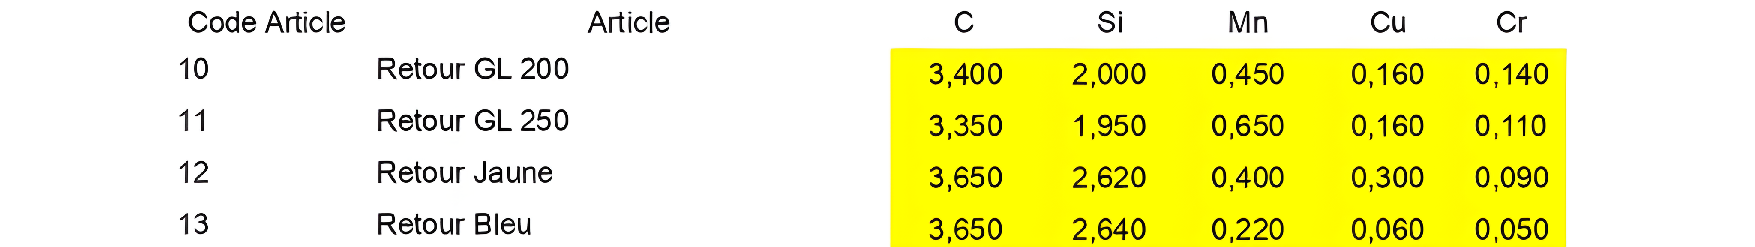
\includegraphics[width=\textwidth]{Images/Recette/Tableau matières premières 1-1.pdf} \\
            \vspace{0.01 cm}
            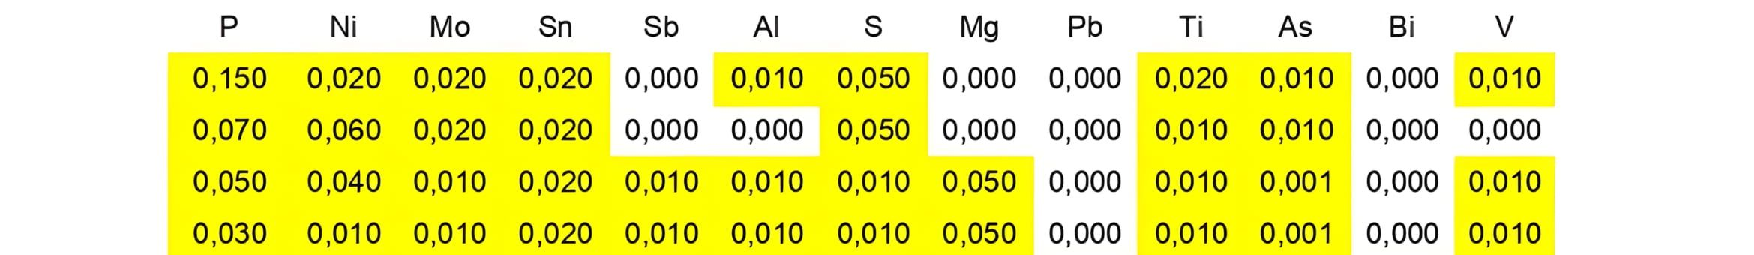
\includegraphics[width=\textwidth]{Images/Recette/Tableau matières premières 1-2.pdf}
        \end{minipage}
    }
    \caption{Illustration du tableau matières premières}
    \label{fig:contraintes1}
\end{figure}



% Les contraintes qualités de la GS 400-15 et de la GS 450-10
\begin{figure}[H]
    \centering
    \adjustbox{width=1.3\textwidth, center}{
        \begin{minipage}{\textwidth}
            \centering
            \includegraphics[width=0.75\paperwidth]{Images/Recette/Contraintes Qualités GS_400_15_1.pdf} \\
            \vspace{0.01 cm}
            \includegraphics[width=0.75\paperwidth]{Images/Recette/Contraintes Qualités GS_400_15_2.pdf}  \\
            \vspace{0.5 cm}
            \includegraphics[width=0.75\paperwidth]{Images/Recette/Contraintes Qualités GS_450_10_1.pdf}  \\
            \vspace{0.01 cm}
            \includegraphics[width=0.75\paperwidth]{Images/Recette/Contraintes Qualités GS_450_10_2.pdf}  
        \end{minipage}
    }
    \caption{Les contraintes qualités de la fonte GS 400-15 et GS 450-10}
    \label{fig:contraintes2}
\end{figure}


% Les contraintes matières premières
\begin{figure}[H]
    \centering
    \begin{adjustbox}{width=1.25\textwidth,center}
        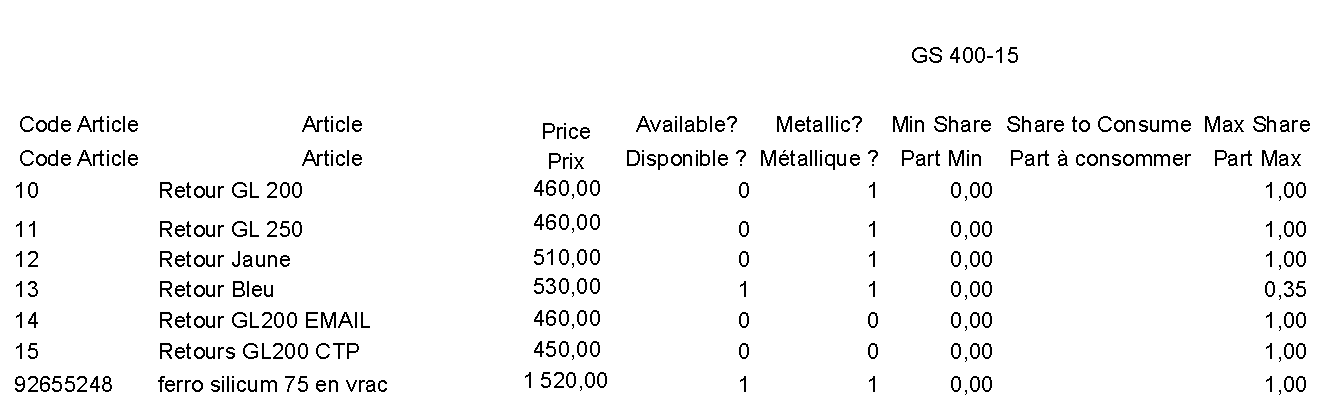
\includegraphics[scale=1]{Images/Recette/Contraintes matières premières 1.pdf}
    \end{adjustbox}
    \caption{Les contraintes matières premières}
    \label{fig:contraintes3}
\end{figure}





%  Les ouputs de l'algos


% La recette de la fonte GS 450-10  de la fonderie
\begin{figure}[H]
    \centering
    \adjustbox{width=1.18\textwidth, center}{
        \begin{minipage}{\textwidth}
            \centering
            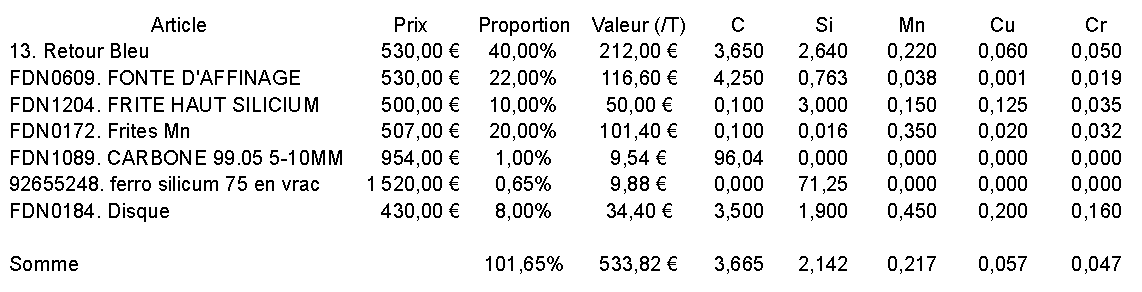
\includegraphics[width=\textwidth]{Images/Recette/Recettes Fonderies GS 450_10_1.pdf} \\
            \vspace{0.01 cm}
            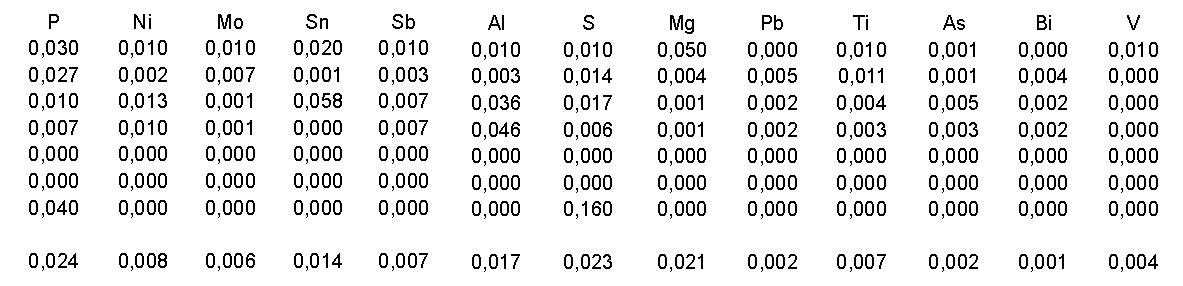
\includegraphics[width=\textwidth]{Images/Recette/Recettes Fonderies GS 450_10_2.pdf}
        \end{minipage}
    }
    \caption{La recette de la fonte GS 450-10 de la fonderie}
    \label{fig:Recette1}
\end{figure}


% La recette de la fonte GS 600-3 de la fonderie
\begin{figure}[H]
    \centering
    \adjustbox{width=1.18\textwidth, center}{
        \begin{minipage}{\textwidth}
            \centering
            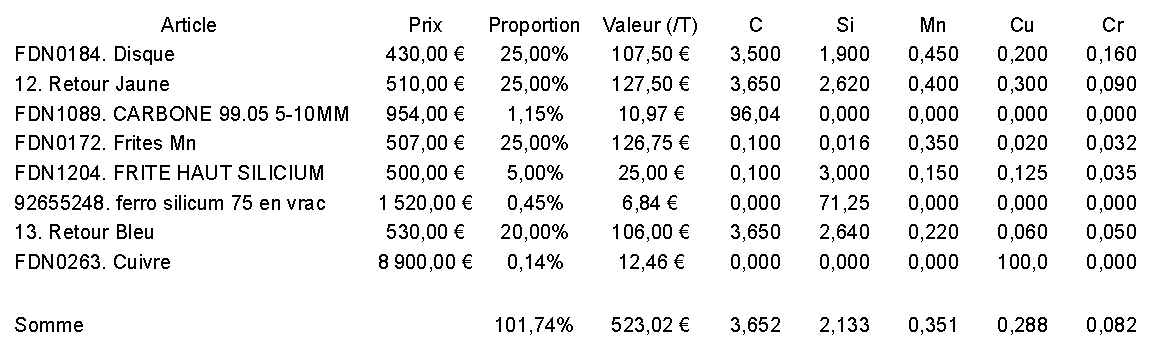
\includegraphics[width=\textwidth]{Images/Recette/Recettes Fonderies GS 600_3_1.pdf} \\
            \vspace{0.01 cm}
            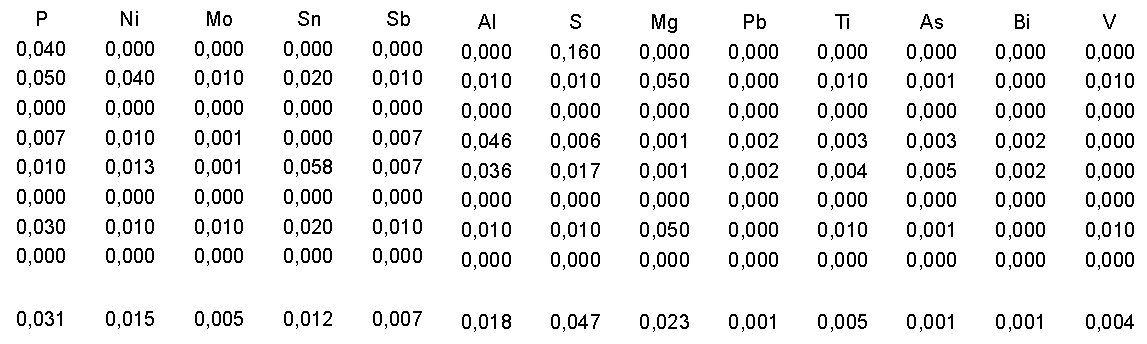
\includegraphics[width=\textwidth]{Images/Recette/Recettes Fonderies GS 600_3_2.pdf}
        \end{minipage}
    }
    \caption{La recette de la fonte GS 600-3 de la fonderie}
    \label{fig:Recette2}
\end{figure}





% Les recettes du simplexe :


% La recette de la fonte GS 450-10 du simplexe 1
\begin{figure}[H]
    \centering
    \adjustbox{width=1.18\textwidth, center}{
        \begin{minipage}{\textwidth}
            \centering
            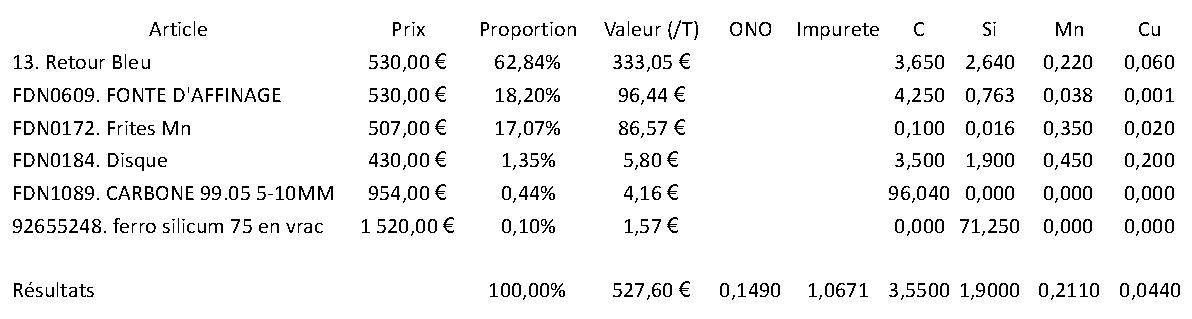
\includegraphics[width=\textwidth]{Images/Recette/Recettes Simplexe 1 GS 450_10_1.pdf} \\
            \vspace{0.01 cm}
            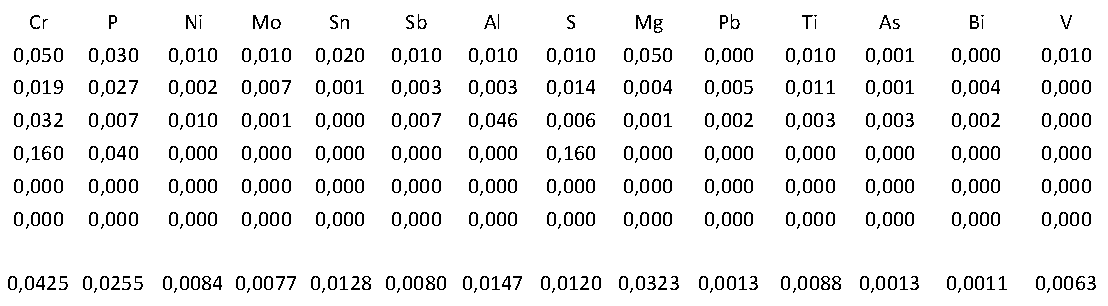
\includegraphics[width=\textwidth]{Images/Recette/Recettes Simplexe 1 GS 450_10_2.pdf}
        \end{minipage}
    }
    \caption{La recette de la fonte GS 450-10 de l'algorithme du simplexe version 1}
    \label{fig:Recette3}
\end{figure}


% La recette de la fonte GS 600-3  du simplexe 1
\begin{figure}[H]
    \centering
    \adjustbox{width=1.18\textwidth, center}{
        \begin{minipage}{\textwidth}
            \centering
            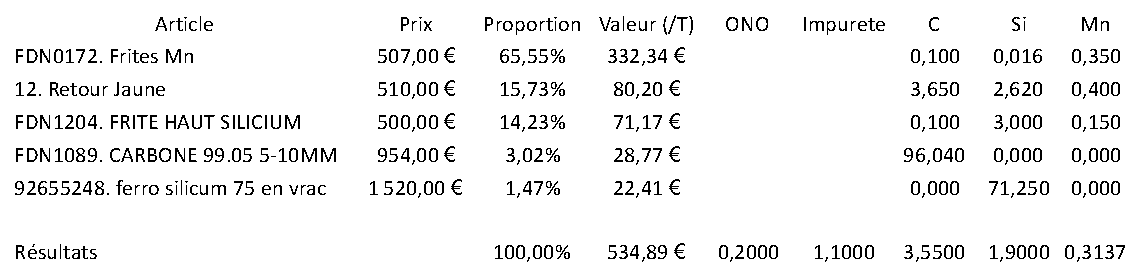
\includegraphics[width=\textwidth]{Images/Recette/Recettes Simplexe 1 GS 600_3_1.pdf} \\
            \vspace{0.01 cm}
            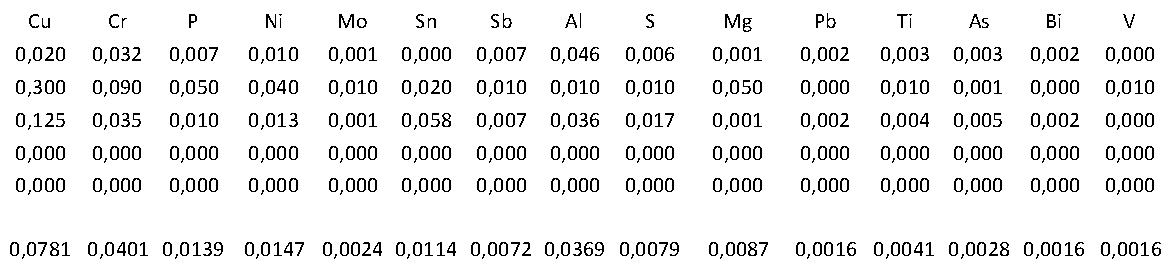
\includegraphics[width=\textwidth]{Images/Recette/Recettes Simplexe 1 GS 600_3_2.pdf}
        \end{minipage}
    }
    \caption{La recette de la fonte GS 600-3 de l'algorithme du simplexe version 1}
    \label{fig:Recette4}
\end{figure}


% La recette de la fonte GS 450-10 du simplexe 2
\begin{figure}[H]
    \centering
    \adjustbox{width=1.18\textwidth, center}{
        \begin{minipage}{\textwidth}
            \centering
            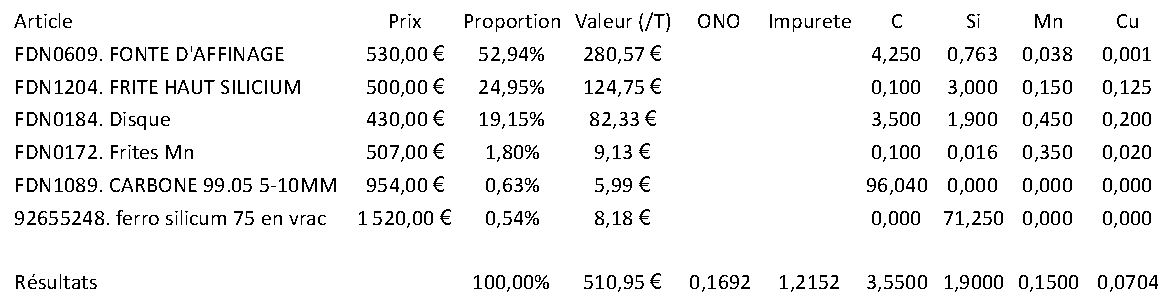
\includegraphics[width=\textwidth]{Images/Recette/Recettes Simplexe 2 GS 450_10_1.pdf} \\
            \vspace{0.01 cm}
            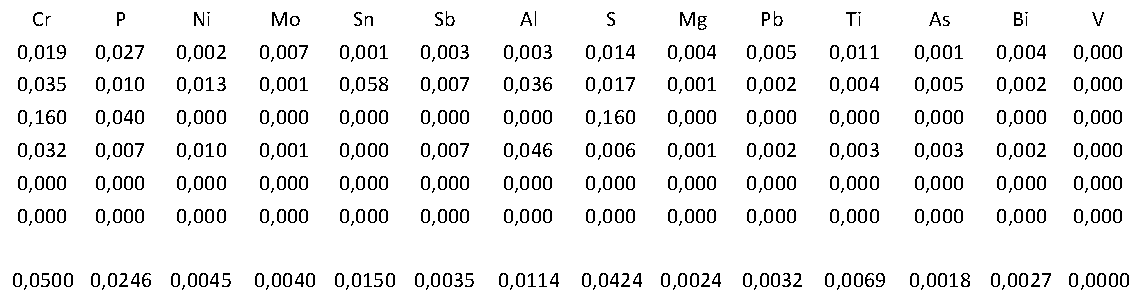
\includegraphics[width=\textwidth]{Images/Recette/Recettes Simplexe 2 GS 450_10_2.pdf}
        \end{minipage}
    }
    \caption{La recette de la fonte GS 450-10 de l'algorithme du simplexe version 2}
    \label{fig:Recette5}
\end{figure}


% La recette de la fonte GS 600-3  du simplexe 2
\begin{figure}[H]
    \centering
    \adjustbox{width=1.18\textwidth, center}{
        \begin{minipage}{\textwidth}
            \centering
            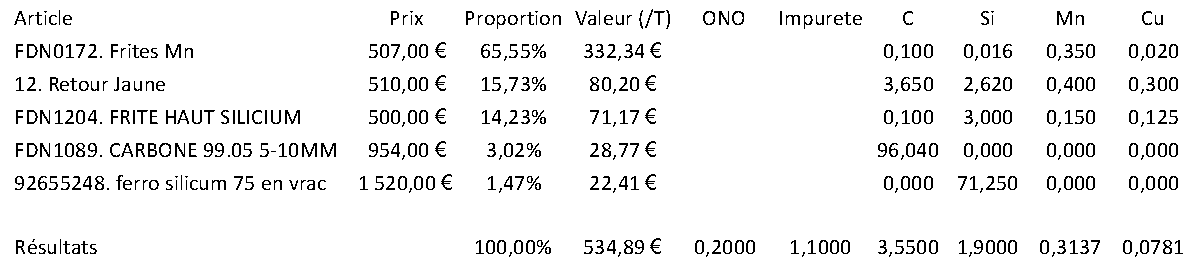
\includegraphics[width=\textwidth]{Images/Recette/Recettes Simplexe 2 GS 600_3_1.pdf} \\
            \vspace{0.01 cm}
            \includegraphics[width=\textwidth]{Images/Recette/Recettes Simplexe 2 GS 600_3_2.pdf}
        \end{minipage}
    }
    \caption{La recette de la fonte GS 600-3 de l'algorithme du simplexe version 2}
    \label{fig:Recette6}
\end{figure}







Pour la GS 450-10 et la GS 600-3, les coûts initiaux des recettes 
proposées par la fonderie sont de 533,82 euros et 523,02 euros 
respectivement. En appliquant la première formulation du problème, 
ces coûts ont été optimisés pour atteindre 527,60 euros pour la GS 450-10 
et 534,89 euros pour la GS 600-3. La deuxième formulation, quant à elle, 
a maintenu un coût proche pour la GS 450-10, tandis qu'elle a permis de 
réduire le coût de la GS 600-3 à 510,90 euros.
Ces résultats montrent un compromis entre le coût et la qualité, où la 
première formulation privilégie l'économie, tandis que la deuxième vise 
une qualité supérieure de la fonte, avec un impact minimal sur les coûts.


\begin{comment}
    
% Les recettes du simplexe 1
\begin{figure}[H]
    \centering
    \adjustbox{width=1.3\textwidth, center}{
        \begin{minipage}{\textwidth}
            \centering
            \includegraphics[width=0.75\paperwidth]{Images/Recette/Recettes Fonderies GS 450_10_1.pdf} \\
            \vspace{0.01 cm}
            \includegraphics[width=0.75\paperwidth]{Images/Recette/Recettes Fonderies GS 450_10_2.pdf}  \\
            \vspace{0.5 cm}
            \includegraphics[width=0.75\paperwidth]{Images/Recette/Recettes Fonderies GS 600_3_1.pdf} \\
            \vspace{0.01 cm}
            \includegraphics[width=0.75\paperwidth]{Images/Recette/Recettes Fonderies GS 600_3_2.pdf}  
        \end{minipage}
    }
    \caption{Les recettes du l'algorithme du simplexe pour les fontes GS 450-10 et GS 600-3}
    \label{fig:Recette2}
\end{figure}


\end{comment}



\section{Le Traitement au Magnésium de la fonte GS}

\subsection{Présentation du problème }



Cette section est consacrée à l'optimisation de la production de fonte à 
graphite sphéroïdal (GS) réalisée sur la ligne de moulage DISAMATIC, en 
particulier au processus de sphéroïdisation. Cette étape critique consiste 
à introduire du magnésium (Mg) dans la fonte avant la coulée, sous forme 
d'alliage, à l'aide d'un fil fourré d'un prix de 1,12 € le mètre.



Avant d'ajouter le fil fourré, la fonte doit d'abord être produite. 
La fonderie dispose de deux fours de fusion d'une capacité de 5 tonnes 
chacun. La préparation du lit de fusion, qui consiste à charger les 
matières premières, prend 25 minutes, tandis que la fusion elle-même 
dure 45 minutes. Il est supposé que la fonte produite par les fours de 
fusion ne contient pas de magnésium.

Une fois la fonte créée, elle est versée dans des poches pour être 
transportée. Deux types de poches sont utilisés : la poche de traitement 
et la poche de coulée, chacune ayant une capacité de 1250 kg de fonte. 
La fonte est ensuite reçue dans le four de coulée.

Concernant le four de coulée, certaines règles spécifiques doivent être 
respectées. Ce four, qui a une capacité maximale de 5 tonnes, doit 
toujours contenir au moins 2500 kg de fonte. Si cette quantité minimale 
n'est pas respectée, le four pourrait être endommagé. Par conséquent, 
la production des moules ne commence qu'après l'ajout de la troisième 
poche de fonte.

Le pourcentage de magnésium dans la fonte doit être maintenu 
entre Mg min = 0,035 \% et Mg max = 0,045 \%. 
Cette contrainte sur la teneur en magnésium 
est essentielle pour garantir la qualité des pièces finales tout en 
minimisant le coût du fil fourré.

Le programme de production journalier varie en fonction du type, de la 
taille et de la quantité des pièces à réaliser. Cela entraîne des 
fluctuations dans le nombre de mottes à produire, la masse des grappes 
et le nombre de moules fabriqués par heure.

En général, une perte de magnésium de eC = 0,0005 \% par minute est 
observée dans le four de coulée. En outre, lors du transfert de la fonte entre 
la cabine de fil fourré et le four de coulée, une perte supplémentaire 
de 0,001 \% par minute est estimée. Le traitement au magnésium dure 
environ 10 minutes, ce qui signifie que la fonte met 10 minutes pour 
passer du processus de fusion au four de coulée.

L'objectif principal est de déterminer la longueur de fil fourré à 
utiliser pour chaque poche de traitement, de manière à ce que le four 
de coulée atteigne le pourcentage maximal de magnésium fixé à 0,045 \%. 
Le second objectif est d'optimiser le moment du lancement de la prochaine 
poche de traitement, en fonction du rythme de production des moules.

Les figures ci-dessous illustrent le processus de traitement de la fonte 
GS pour les trois premières poches.


% Le Traitement GS


% Les Poches MG 1 et 2 et 3
\begin{figure}[H]
    \centering
    \begin{adjustbox}{height=0.49\textheight,width=1.25\textwidth,center}
        \includegraphics{Images/Mg/Poche 1.pdf} % Première image
    \end{adjustbox}
    
    \vspace{0.01cm} % Espacement entre les images
    
    \begin{adjustbox}{height=0.49\textheight,width=1.25\textwidth,center}
        \includegraphics{Images/Mg/Poche 2.pdf} % Deuxième image
    \end{adjustbox}

    \caption{Le Traitement au MG des Poche 1 et Poche 2}
    \label{fig:Poche1Et2}
\end{figure}



\begin{figure}[H]
    \centering
    \begin{adjustbox}{width=1.3\textwidth,center}
        \includegraphics{Images/Mg/Poche 3.pdf}
    \end{adjustbox}
    \caption{Le Traitement au MG de la Poche 3}
    \label{fig:Poche3}
\end{figure}



\subsection{Implémentation et Résultats}


Ce problème peut être divisé en deux phases distinctes :

\begin{enumerate}
    \item \textbf{Régime transitoire} : Cette phase correspond à l'ajout des trois 
    premières poches de fonte dans le four de coulée. L'objectif est 
    d'atteindre un pourcentage de magnésium (Mg) de 0,045 \% après l'ajout 
    de la troisième poche. Il s'agit donc de déterminer la longueur de fil 
    fourré à introduire dans chaque poche de traitement pour atteindre 
    cette cible.
    
    \item \textbf{Régime établi} : Une fois le régime transitoire terminé, 
    la production des pièces commence. Durant cette phase, il est crucial 
    de déterminer le moment optimal pour lancer le traitement des poches 
    suivantes, tout en calculant la longueur de fil fourré à ajouter à 
    chaque fois pour maintenir la teneur en magnésium dans les limites 
    fixées.
\end{enumerate}

Pour déterminer la quantité d'alliage au magnésium (ou de fil fourré dans 
notre cas) à introduire dans chaque poche, on utilise la relation 
empirique suivante :

$$
\mathbf{Q} = \mathbf{P} \cdot \frac{0.76 (\mathbf{S} - 0.01) + \mathbf{K} + \mathbf{t} \cdot \mathbf{eP}}{\frac{\mathbf{R} \cdot \mathbf{Mg}}{100}} \cdot \left(\frac{\mathbf{T}}{1450}\right)^2
$$

\textbf{Variables et paramètres :}

\begin{itemize}
    \item \textbf{Q} : Quantité d'alliage au magnésium à utiliser (en kg)
    \item \textbf{P} : Poids de fonte à traiter (en kg)
    \item \textbf{S} : Taux de soufre de la fonte de base (en \%)
    \item \textbf{t} : Temps de séjour prévu pour la fonte après traitement (en minutes)
    \item \textbf{eP} : Pourcentage de perte de magnésium par minute dans la poche (\%)
    \item \textbf{T} : Température de la fonte au moment du traitement (en degrés Celsius)
    \item \textbf{R} : Rendement en magnésium de l'opération (en \%)
    \item \textbf{Mg} : Taux de magnésium dans l'alliage (en \%)
    \item \textbf{K} : Quantité de magnésium résiduel nécessaire pour que le graphite soit sous forme sphéroïdal (en \%)
\end{itemize}



Dans la phase transitoire, l'objectif est de déterminer les 
paramètres $\mathbf{K_1}$ , $\mathbf{K_2}$ et $\mathbf{K_3}$ afin d'assurer 
que la teneur en magnésium (Mg) dans le four de coulée respecte les 
seuils souhaités après l'ajout de la troisième poche. Pour garantir 
cela, nous imposons la condition suivante :

$$
K_{\text{max}} \cdot (P_1 + P_2 + P_3) = \mathbf{K_1} \cdot P_1 - P_1 \cdot 2 \cdot \text{mg}_{\text{perdu}} + \mathbf{K_2}  \cdot P_2 - P_2 \cdot \text{mg}_{\text{perdu}} + \mathbf{K_3}  \cdot P_3
$$

où :
$\text{mg}_{\text{perdu}} = \text{DureeTraitement} \times eC$
Les variables $P_1$, $P_2$, $P_3$ sont les masses de fonte des trois 
poches, et $K_{\text{max}} = 0.045$

Pour utiliser la même longueur de fil fourré dans chaque 
poche, on ajoute les conditions supplémentaires : $Q_1 = Q_2$ 
et $Q_1 = Q_3$. Cela génère un système de trois équations avec trois 
inconnues.



Dans le cadre du régime établi, il est nécessaire d'ajouter de la fonte 
pour deux raisons principales :
\begin{enumerate}
    \item Le pourcentage de magnésium (Mg) devient insuffisant pour maintenir la qualité de la production.
    \item La quantité de fonte disponible dans le four de maintien approche du minimum critique.
\end{enumerate}

Afin d'anticiper ces situations, nous avons calculé le temps disponible 
avant qu'une intervention ne soit nécessaire, à partir du taux de perte 
de magnésium par minute dans le four de coulée et du rythme de production 
des moules.



Le calcul du temps avant que la fonte disponible ne devienne insuffisante 
est basé sur la consommation de fonte par minute, liée au nombre de moules 
produits par heure et à la masse de fonte par moule. Voici les étapes 
détaillées :

\begin{lstlisting}[language=Python, caption=Calcul du temps avant épuisement de la fonte]
# Temps admissible avant l'ajout de fonte dans le four de maintien,
# pour éviter d'atteindre la quantité minimale de fonte (en kg).
consommation_fonte_min = nb_moules_heure * masse_grappe / 60  # kg/min
fonte_four_consommable = masse_fonte_coulee - masse_fonte_coulee_min
temps_epuis_fonte = fonte_four_consommable / consommation_fonte_min
delai_avt_traitement_fonte_four = temps_epuis_fonte - temps_traitement
\end{lstlisting}

\begin{itemize}
    \item \textbf{consommation\_fonte\_min} : Consommation de fonte en kg par minute, basée sur le rythme de production des moules.
    \item \textbf{fonte\_four\_consommable} : Quantité de fonte disponible avant d'atteindre le seuil critique.
    \item \textbf{temps\_epuis\_fonte} : Temps estimé avant que la fonte ne soit épuisée.
    \item \textbf{delai\_avt\_traitement\_fonte\_four} : Délai disponible avant de devoir ajouter de la fonte, en tenant compte du temps de traitement.
\end{itemize}


Le pourcentage de magnésium dans la fonte diminue progressivement au 
cours du processus de production. Le temps avant que ce pourcentage 
atteigne un seuil critique est calculé de la manière suivante :

\begin{lstlisting}[language=Python, caption=Calcul du temps avant épuisement du magnésium]
# Temps admissible avant l'ajout de magnésium dans le four de maintien,
# pour éviter d'atteindre le pourcentage minimal de Mg.
pct_mg_four_consommable = pct_mg_fonte_coulee - pct_mg_fonte_coulee_min
temps_epuis_mg = pct_mg_four_consommable / pct_perdu_mg_coulee_min
delai_avt_traitement_mg_four = temps_epuis_mg - temps_traitement
\end{lstlisting}

\begin{itemize}
    \item \textbf{pct\_mg\_four\_consommable} : Pourcentage de magnésium consommable avant d'atteindre le seuil minimal.
    \item \textbf{temps\_epuis\_mg} : Temps estimé avant que le pourcentage de magnésium ne devienne insuffisant.
    \item \textbf{delai\_avt\_traitement\_mg\_four} : Délai disponible avant de devoir ajouter du magnésium.
\end{itemize}



Le moment optimal pour lancer le traitement est déterminé en prenant le 
minimum entre le délai avant que la fonte ne soit épuisée et le délai 
avant que le pourcentage de magnésium ne devienne insuffisant. Cela 
garantit que l'intervention se fait au moment opportun pour éviter tout 
dysfonctionnement du processus de production.

\begin{lstlisting}[language=Python, caption=Calcul du délai avant traitement optimal]
delai_avt_traitement = min(temps_epuis_fonte, delai_avt_traitement_mg_four)
\end{lstlisting}


\section*{Conclusion et Perspectives}

Pour conclure cette partie, il est notable qu'une grande différence a 
été observée entre le calcul théorique de la longueur de fil fourré, 
estimée entre 15 et 20 mètres, et la longueur mesurée en pratique, qui 
s'élève à 68 mètres. Cet écart significatif suggère que les estimations 
théoriques pourraient être améliorées en affinant les paramètres utilisés 
dans les calculs et/ou la démarche suivie pour repondre au problème.

Pour les travaux futurs, il serait bénéfique d'intégrer des variables 
supplémentaires afin de mieux modéliser le système. En particulier, il 
serait pertinent de prendre en compte :
\begin{itemize}
    \item La durée du changement de moules pour chaque pièce.
    \item La durée des pannes indéterminées qui peuvent survenir.
\end{itemize}


\section*{Conclusion générale}


Ce stage, divisé en trois grandes parties, a permis d'explorer plusieurs 
aspects cruciaux de la production de fonte à travers une approche 
mathématique et statistique. La première partie a été consacrée à l'étude 
statistique, comprenant le nettoyage et le pré-traitement des données. 
La deuxième partie a porté sur la détermination de la recette optimale 
en utilisant l'algorithme du simplexe. Enfin, la troisième partie s'est 
concentrée sur l'optimisation du processus de sphérodisation, notamment 
en déterminant la longueur optimale du fil fourré et le timing idéal pour 
l'ajout de chaque poche de traitement.

L'utilisation de l'algorithme du simplexe a permis de développer une 
méthode automatisée pour calculer les recettes optimales en fonction des 
contraintes spécifiques du problème. Les résultats obtenus sont prometteurs
pour des applications futures sur le terrain. Deux approches principales 
ont été mises en avant : l'une axée sur la minimisation des coûts, et 
l'autre sur la combinaison de la minimisation des coûts avec l'amélioration
de la qualité de la fonte. 

En revanche, l'étude statistique visant à évaluer la conformité de la 
fonte et le traitement au magnésium n'a pas fourni des résultats 
entièrement satisfaisants en raison du manque de données et d'informations.
Malgré cela, des indicateurs comme l'impureté et la pureté ONO se sont 
révélés être les critères les plus pertinents pour évaluer la qualité de 
la fonte.

Concernant la sphérodisation, un écart a été observé entre les données 
théoriques et pratiques, soulignant la nécessité d'une analyse plus 
approfondie pour affiner ces paramètres dans un contexte opérationnel.

% En conclusion, ce stage a permis de mettre en place des outils et des 
% méthodes d'optimisation.

\begin{comment}
    
    - Obtention des images inputs, outpouts Optimisation de la Presentations
Dans le drive , exporter en pdf avec parametre Paysage, Statement, dessus puis bas



Peux-tu amélioré la présentation en donnant les éléments les plus pertinents sous forme de phrase ou en faisant autrement, notamment en 
en fournissant une explication claire et fluide pour un rapport de stage de master en math applique 
    
Peux-tu reformuler pour le rendre lisible et claire :


Peux-tu reformuler pour le rendre lisible et claire pour un rapport de 
stage de master en math applique ,en modifiant si cela te semble meilleur :



Pour une section d'un rapport de stage d'un étudiant de master en math 
appliquée, peux-tu repondre à ses différents questions de manière precises,
claire et concis :


Tu es un étudiant en dernière année de master de  mathématiques appliquées et tu dois pour un rapport de stage inclure une section qui présente et explique l'algorithme du simplexe.
As-tu des idées sur comment t'y prendre ? Si oui , fais-le ! 


\end{comment}


\begin{comment}
    
    Phase 1 :
\section*{Résumé de la phase d'initialisation du simplexe (phase 1)}

On note $F_{aux} \) la valeur de la fonction objectif du problème auxiliaire (PLA) à la fin du simplexe, c'est-à-dire 
\[ F_{aux} = \min \sum_{j=1}^{n} x_j \]

\begin{enumerate}
    \item Si \( F_{aux} = 0 \) et \( x_0 = 0 \), on passe à la phase 2 du simplexe.
    \item Si \( F_{aux} = 0 \) et \( x_0 > 0 \), on supprime les lignes et colonnes associées aux \( x_i \), et on passe à la phase 2 avec \( q \).
    \item Si \( F_{aux} > 0 \), alors pas de solution réalisable pour le DPL (phase).
\end{enumerate}



\section*{Définition 4.2}

Soit $B \subset \{1, \cdots, n\}$ un ensemble d'indices avec $\text{card}(B) = m$ tel que les colonnes $A_j$, $j \in B$, de $A$ sont linéairement indépendantes. Autrement dit, la matrice carrée $A_B$ formée des colonnes $A_j$, $j \in B$, est inversible. On dit que l'ensemble $B$ des indices est une base.

Les variables $X_B = (x_j)_{j \in B}$ sont appelées variables de base.

Les variables $X_H = (x_j)_{j \notin B}$ sont appelées variables hors-base.

On notera $H = \{j \in \{1, \cdots, n\}, j \notin B\}$ l'ensemble des indices correspondants aux variables hors-base.
\section*{Résumé de la méthode du simplexe en phase 2 (progression)}

\begin{enumerate}
    \item \textbf{Variables de base réalisables et coûts réduits :}
    \begin{itemize}
        \item Calcul des variables de base réalisables : étant donné $A = (A_B | A_H)$, on calcule les variables de base réalisables $X_B = A_B^{-1}b \geq 0$.
        \item Calcul des coûts réduits : $\lambda_H = c_H - c_B A_B^{-1} A_H$.
        \item Si $\lambda_H \leq 0$ alors $X_p$ est une solution optimale (arrêt de l'algorithme).
    \end{itemize}
    \item \textbf{Variable entrante $e$ :} détermination de l'indice $e = \arg\max_i \{ \lambda_H \}_i$ tel que $\lambda_H > 0$.
    \item \textbf{Variable sortante $s$ :}
    \begin{itemize}
        \item Calcul de $z = A_B^{-1} A^e$.
        \item Détermination de l'indice $s = \arg\min_i \left\{ \frac{(X_B)_i}{z_i} \right\}$ tel que $z_i > 0$.
    \end{itemize}
    \item On obtient une nouvelle base $B^*$ et une nouvelle matrice $A_B^*$ dans laquelle la colonne $A^e$ remplace la colonne $A_s$. Calcul de $A_B^{-1}$ et retour à l'étape 1 avec la base $B^*$ au lieu de $B$.
\end{enumerate}

% sudo apt-get install texlive-full

\end{comment}







\begin{thebibliography}{9}

\bibitem{FonderieNiederbronn}
Fonderie de Niederbronn. \emph{Site web de la Fonderie de Niederbronn}. Accessible à l'adresse : \url{https://www.fonderie-de-niederbronn.com/}.

\bibitem{Reynaud}
Alain Reynaud. \emph{Oligo-éléments \& fontes}. ETIF, 2009.

\bibitem{Scheid}
J.-F Scheid. \emph{Cours de Graphes et Recherche Opérationnelle}. Disponible en ligne : \url{https://scheid.perso.math.cnrs.fr/Enseignement/coursGRO_PL.pdf}.

\bibitem{CTIF}
Centre Technique des Industries de la Fonderie. \emph{Fabrication de la fonte à graphite sphéroïdal par les procédés au magnésium (Addition à la poche d'alliages au magnésium)}, juin 1972.

\bibitem{Contifonte S.A.}
Sorelmetal. \emph{Principes et applications de l'analyse des fontes et Méthodes d'analyse des fontes}, 2005.


\bibitem{ATF et CPE}
Franck Kootz \emph{Les Fours à induction, Aspects Métallurgiques au four}, 2023.


\bibitem{Rio Tinto Fer & Titane inc.}
Sorelmetal. \emph{Fonte à graphite sphéroïdal (Fonte GS)}. Disponible en ligne : \url{https://www.soudeurs.com/telechargements/130-sorelmetal_fonte_gs_Deddi-Fr.pdf}.


\bibitem{JDAY}
Rawen Jday. \emph{Caractérisation microstructurale du graphite sphéroïdal formé lors de la
solidification et à l'état solide}. Thèse de doctorat, Université Toulouse, 2017. Disponible en ligne : \url{https://theses.hal.science/tel-04228112v1/file/JDAY_Rawen.pdf}.

\end{thebibliography}

\begin{appendices}
    \section{La recette optimale}
    Voici les recettes d'autres fonte GS :

    


    %  Les ouputs de l'algos


% La recette de la fonte GS 400-15  de la fonderie
\begin{figure}[H]
    \centering
    \adjustbox{width=1.18\textwidth, center}{
        \begin{minipage}{\textwidth}
            \centering
            \includegraphics[width=\textwidth]{Images/Recette/Recettes Fonderies GS 400_15_1.pdf} \\
            \vspace{0.01 cm}
            \includegraphics[width=\textwidth]{Images/Recette/Recettes Fonderies GS 400_15_2.pdf}
        \end{minipage}
    }
    \caption{La recette de la fonte GS 400-15 de la fonderie}
    \label{fig:Recette7}
\end{figure}


% La recette de la fonte GS 500-7 de la fonderie
\begin{figure}[H]
    \centering
    \adjustbox{width=1.18\textwidth, center}{
        \begin{minipage}{\textwidth}
            \centering
            \includegraphics[width=\textwidth]{Images/Recette/Recettes Fonderies GS 500_7_1.pdf} \\
            \vspace{0.01 cm}
            \includegraphics[width=\textwidth]{Images/Recette/Recettes Fonderies GS 500_7_2.pdf}
        \end{minipage}
    }
    \caption{La recette de la fonte GS 500-7 de la fonderie}
    \label{fig:Recette8}
\end{figure}





% Les recettes du simplexe :


% La recette de la fonte GS 400-15 du simplexe 1
\begin{figure}[H]
    \centering
    \adjustbox{width=1.18\textwidth, center}{
        \begin{minipage}{\textwidth}
            \centering
            \includegraphics[width=\textwidth]{Images/Recette/Recettes Simplexe 1 GS 400_15_1.pdf} \\
            \vspace{0.01 cm}
            \includegraphics[width=\textwidth]{Images/Recette/Recettes Simplexe 1 GS 400_15_2.pdf}
        \end{minipage}
    }
    \caption{La recette de la fonte GS 400-15 de l'algorithme du simplexe version 1}
    \label{fig:Recette9}
\end{figure}


% La recette de la fonte GS 500-7  du simplexe 1
\begin{figure}[H]
    \centering
    \adjustbox{width=1.18\textwidth, center}{
        \begin{minipage}{\textwidth}
            \centering
            \includegraphics[width=\textwidth]{Images/Recette/Recettes Simplexe 1 GS 500_7_1.pdf} \\
            \vspace{0.01 cm}
            \includegraphics[width=\textwidth]{Images/Recette/Recettes Simplexe 1 GS 500_7_2.pdf}
        \end{minipage}
    }
    \caption{La recette de la fonte GS 500-7 de l'algorithme du simplexe version 1}
    \label{fig:Recette10}
\end{figure}


% La recette de la fonte GS 400-15 du simplexe 2
\begin{figure}[H]
    \centering
    \adjustbox{width=1.18\textwidth, center}{
        \begin{minipage}{\textwidth}
            \centering
            \includegraphics[width=\textwidth]{Images/Recette/Recettes Simplexe 2 GS 400_15_1.pdf} \\
            \vspace{0.01 cm}
            \includegraphics[width=\textwidth]{Images/Recette/Recettes Simplexe 2 GS 400_15_2.pdf}
        \end{minipage}
    }
    \caption{La recette de la fonte GS 400-15 de l'algorithme du simplexe version 2}
    \label{fig:Recette11}
\end{figure}


% La recette de la fonte GS 500-7  du simplexe 2
\begin{figure}[H]
    \centering
    \adjustbox{width=1.18\textwidth, center}{
        \begin{minipage}{\textwidth}
            \centering
            \includegraphics[width=\textwidth]{Images/Recette/Recettes Simplexe 2 GS 500_7_1.pdf} \\
            \vspace{0.01 cm}
            \includegraphics[width=\textwidth]{Images/Recette/Recettes Simplexe 2 GS 500_7_2.pdf}
        \end{minipage}
    }
    \caption{La recette de la fonte GS 500-7 de l'algorithme du simplexe version 2}
    \label{fig:Recette12}
\end{figure}

\end{appendices}

\end{document}